% thesis.tex
% This is the main file, which calls up preamble.tex, frontmatter.tex, and thesis.bib as needed.

% Frontmatter shortcuts; note the extra space at the end, which is unfortunately necessary:
\newcommand\myname{William Huanshan Chuang}
\newcommand\mytitle{The Hausdorff Dimension of Limit Sets of Well-distributed Schottky Groups} % The graduate division requires this to be in caps.
%The Computation of Hausdorff dimension for Bounds on Volume of some Algebraic Curves via its exponent of Poincar\'{e} Series
%Automorphic Function and Poincar\'{e} Series in Algebraic Curves
%The Computation of the Critical Exponent of Poincar\'{e} Series via spectral theory and the geometry of Kleinian groups with Applications
\newcommand\mydegree{Master of Arts} % change to  Master of Science if applicable
\newcommand\myfield{Mathematics} % e.g., Mathematics
\newcommand\thismonth{May } % graduation month: May / August / December
\newcommand\thisyear{2022 } % e.g., 2014

% Shortcuts (add your own...):
\newcommand{\N}{\mathbb{N}}
\newcommand{\Z}{\mathbb{Z}}
\newcommand{\Q}{\mathbb{Q}}
\newcommand{\R}{\mathbb{R}}
\newcommand{\C}{\mathbb{C}}





% One of the following two has to be commented out:
%\include{draftpreamble}  % eco-friendly draft version
%\include{preamble}   % final version, formatted according to the Graduate Division's guidelines

% preamble.tex, to be used with thesis.tex
% This contains the TeX definitions for layout, style, etc., as well as the first few pages of your thesis: title page, copyright page, approval page, abstract, acknowledgments, tables of contents, tables, and figures.
% The layout commands should give the correct margins according to the graduate division's guidelines

%%%%% TeX class and packages

\documentclass[12pt,oneside]{sfsuthesis}

\usepackage{tikz-cd}

%Python Code Listing
\usepackage[utf8]{inputenc}
\usepackage[english]{babel}
\usepackage[T1]{fontenc}


\usepackage{tcolorbox}
\usepackage{xcolor}
\definecolor{maroon}{cmyk}{0, 0.87, 0.68, 0.32}
\definecolor{halfgray}{gray}{0.55}
\definecolor{ipython_frame}{RGB}{207, 207, 207}
\definecolor{ipython_bg}{RGB}{247, 247, 247}
\definecolor{ipython_red}{RGB}{186, 33, 33}
\definecolor{ipython_green}{RGB}{0, 128, 0}
\definecolor{ipython_cyan}{RGB}{64, 128, 128}
\definecolor{ipython_purple}{RGB}{170, 34, 255}

\usepackage{hyperref}

    
\usepackage{listings}
\lstset{
    breaklines=true,
    %
    extendedchars=true,
    literate=
    {á}{{\'a}}1 {é}{{\'e}}1 {í}{{\'i}}1 {ó}{{\'o}}1 {ú}{{\'u}}1
    {Á}{{\'A}}1 {É}{{\'E}}1 {Í}{{\'I}}1 {Ó}{{\'O}}1 {Ú}{{\'U}}1
    {à}{{\`a}}1 {è}{{\`e}}1 {ì}{{\`i}}1 {ò}{{\`o}}1 {ù}{{\`u}}1
    {À}{{\`A}}1 {È}{{\'E}}1 {Ì}{{\`I}}1 {Ò}{{\`O}}1 {Ù}{{\`U}}1
    {ä}{{\"a}}1 {ë}{{\"e}}1 {ï}{{\"i}}1 {ö}{{\"o}}1 {ü}{{\"u}}1
    {Ä}{{\"A}}1 {Ë}{{\"E}}1 {Ï}{{\"I}}1 {Ö}{{\"O}}1 {Ü}{{\"U}}1
    {â}{{\^a}}1 {ê}{{\^e}}1 {î}{{\^i}}1 {ô}{{\^o}}1 {û}{{\^u}}1
    {Â}{{\^A}}1 {Ê}{{\^E}}1 {Î}{{\^I}}1 {Ô}{{\^O}}1 {Û}{{\^U}}1
    {œ}{{\oe}}1 {Œ}{{\OE}}1 {æ}{{\ae}}1 {Æ}{{\AE}}1 {ß}{{\ss}}1
    {ç}{{\c c}}1 {Ç}{{\c C}}1 {ø}{{\o}}1 {å}{{\r a}}1 {Å}{{\r A}}1
    {€}{{\EUR}}1 {£}{{\pounds}}1
}

%%
%% Python definition (c) 1998 Michael Weber
%% Additional definitions (2013) Alexis Dimitriadis
%% modified by me (should not have empty lines)
%%
\lstdefinelanguage{iPython}{
    morekeywords={access,and,break,class,continue,def,del,elif,else,except,exec,finally,for,from,global,if,import,in,is,lambda,not,or,pass,print,raise,return,try,while},%
    %
    % Built-ins
    morekeywords=[2]{abs,all,any,basestring,bin,bool,bytearray,callable,chr,classmethod,cmp,compile,complex,delattr,dict,dir,divmod,enumerate,eval,execfile,file,filter,float,format,frozenset,getattr,globals,hasattr,hash,help,hex,id,input,int,isinstance,issubclass,iter,len,list,locals,long,map,max,memoryview,min,next,object,oct,open,ord,pow,property,range,raw_input,reduce,reload,repr,reversed,round,set,setattr,slice,sorted,staticmethod,str,sum,super,tuple,type,unichr,unicode,vars,xrange,zip,apply,buffer,coerce,intern},%
    %
    sensitive=true,%
    morecomment=[l]\#,%
    morestring=[b]',%
    morestring=[b]",%
    %
    morestring=[s]{'''}{'''},% used for documentation text (mulitiline strings)
    morestring=[s]{"""}{"""},% added by Philipp Matthias Hahn
    %
    morestring=[s]{r'}{'},% `raw' strings
    morestring=[s]{r"}{"},%
    morestring=[s]{r'''}{'''},%
    morestring=[s]{r"""}{"""},%
    morestring=[s]{u'}{'},% unicode strings
    morestring=[s]{u"}{"},%
    morestring=[s]{u'''}{'''},%
    morestring=[s]{u"""}{"""},%
    %
    % {replace}{replacement}{lenght of replace}
    % *{-}{-}{1} will not replace in comments and so on
    literate=
    {á}{{\'a}}1 {é}{{\'e}}1 {í}{{\'i}}1 {ó}{{\'o}}1 {ú}{{\'u}}1
    {Á}{{\'A}}1 {É}{{\'E}}1 {Í}{{\'I}}1 {Ó}{{\'O}}1 {Ú}{{\'U}}1
    {à}{{\`a}}1 {è}{{\`e}}1 {ì}{{\`i}}1 {ò}{{\`o}}1 {ù}{{\`u}}1
    {À}{{\`A}}1 {È}{{\'E}}1 {Ì}{{\`I}}1 {Ò}{{\`O}}1 {Ù}{{\`U}}1
    {ä}{{\"a}}1 {ë}{{\"e}}1 {ï}{{\"i}}1 {ö}{{\"o}}1 {ü}{{\"u}}1
    {Ä}{{\"A}}1 {Ë}{{\"E}}1 {Ï}{{\"I}}1 {Ö}{{\"O}}1 {Ü}{{\"U}}1
    {â}{{\^a}}1 {ê}{{\^e}}1 {î}{{\^i}}1 {ô}{{\^o}}1 {û}{{\^u}}1
    { }{{\^A}}1 {Ê}{{\^E}}1 {Î}{{\^I}}1 {Ô}{{\^O}}1 {Û}{{\^U}}1
    {œ}{{\oe}}1 {Œ}{{\OE}}1 {æ}{{\ae}}1 {Æ}{{\AE}}1 {ß}{{\ss}}1
    {ç}{{\c c}}1 {Ç}{{\c C}}1 {ø}{{\o}}1 {å}{{\r a}}1 {Å}{{\r A}}1
    {€}{{\EUR}}1 {£}{{\pounds}}1
    %
    {^}{{{\color{ipython_purple}\^{}}}}1
    {=}{{{\color{ipython_purple}=}}}1
    %
    {+}{{{\color{ipython_purple}+}}}1
    {*}{{{\color{ipython_purple}$^\ast$}}}1
    {/}{{{\color{ipython_purple}/}}}1
    %
    {+=}{{{+=}}}1
    {-=}{{{-=}}}1
    {*=}{{{$^\ast$=}}}1
    {/=}{{{/=}}}1,
    literate=
    *{-}{{{\color{ipython_purple}-}}}1
     {?}{{{\color{ipython_purple}?}}}1,
    %
    identifierstyle=\color{black}\ttfamily,
    commentstyle=\color{ipython_cyan}\ttfamily,
    stringstyle=\color{ipython_red}\ttfamily,
    keepspaces=true,
    showspaces=false,
    showstringspaces=false,
    %
    rulecolor=\color{ipython_frame},
    frame=single,
    frameround={t}{t}{t}{t},
    framexleftmargin=6mm,
    numbers=left,
    numberstyle=\tiny\color{halfgray},
    %
    %
    backgroundcolor=\color{ipython_bg},
    %   extendedchars=true,
    basicstyle=\scriptsize,
    keywordstyle=\color{ipython_green}\ttfamily,
}



\usepackage{amsthm,amsmath,amssymb,amsfonts,latexsym,graphicx,enumerate,setspace,verbatim,tocloft,rotating}
%\usepackage{color}                    % For creating colored text and background
%\usepackage{hyperref}                 % For creating hyperlinks in cross references
% other possibly useful packages: textcomp,mathrsfs,amscd,epsfig,euscript,cancel

%%%%% Layout
% These numbers might depend on your printer. Check the margins and compare them to the Graduate Division's
% guidelines. If there's something off, try playing with the numbers...
%
% For chapters:
%     Must have a minimum of 1.5in margin on left and 1in on all other sides.  Where there are page numbers
%     (whether on top or bottom), must have one additional inch between the page number and the text, for a
%     total of 2in between the edge of the paper and the text.
% For frontmatter pages:
%     The same margin numbers generally work, except for the Title Page, so you will notice that we use
%     some numbers for \textheight and \footskip right here, and then change them below, right after
%     generating the Title Page.

\hoffset=.5in 
\oddsidemargin=0in   % = 1in because LaTeX adds 1in
\evensidemargin=0in  % = 1in because LaTeX adds 1in
\topmargin=0in       % = 1in because LaTeX adds 1in
\headheight=0in
\headsep=1in         % Distance from top of pagenum (for page numbers at top-right corner of page) to text
\footskip=1.2in      % Distance from bottom of text to the page number (for page number at bottom of page)
\textwidth=5.9in     % Should be 6in, but use 5.9in to be conservative
\textheight=8.0in    % Best for Title Page (will change after the Title Page)

\pagestyle{plain}

\doublespacing

%%%%% Style of theorems, definitions, examples, equations, etc.

\theoremstyle{plain} % Heading is bold, text italic.
\newtheorem{theorem}{Theorem}[chapter]
\newtheorem{lemma}[theorem]{Lemma}
\newtheorem{proposition}[theorem]{Proposition}
\newtheorem{corollary}[theorem]{Corollary}
\newtheorem{conjecture}{Conjecture}[chapter]

\theoremstyle{definition}  % Heading is bold, text is roman
\newtheorem{definition}{Definition}[chapter]
\newtheorem{example}{Example}[chapter]

\theoremstyle{remark}  % Heading is italic, text is roman
\newtheorem*{remark}{Remark}
\newtheorem*{note}{Note}
\newtheorem{claim}{Claim}[chapter]

%%%%%%from math 729

\usepackage[]{algorithm2e}
\usepackage{graphicx,float}
\usepackage{tikz}
\usetikzlibrary{graphs,graphs.standard,quotes}
\usepackage{multicol}
\usepackage{capt-of}

%%%%flowchart
\usetikzlibrary{shapes.geometric, arrows}
\tikzstyle{startstop} = [rectangle, rounded corners, minimum width=3cm, minimum height=1cm, text width=25em,text centered, draw=black, fill=yellow!30, inner sep=10pt]
\tikzstyle{io} = [trapezium, trapezium left angle=70, trapezium right angle=110, minimum width=3cm, minimum height=1cm, text centered, draw=black, fill=blue!30]
\tikzstyle{process} = [rectangle, minimum width=3cm, minimum height=1cm, text width=15em, text centered, draw=black, fill=orange!30, inner sep=10pt]
%\tikzstyle{decision} = [diamond, minimum width=3cm, minimum height=1cm, text centered, draw=black, fill=green!30]
\tikzstyle{arrow} = [thick,->,>=stealth]

\tikzstyle{decision} = [rectangle, rounded corners, draw, fill=blue!20, 
    text width=15em, text badly centered, node distance=2.2cm, inner sep=10pt]
\tikzstyle{block} = [rectangle, draw, fill=blue!20, 
    text width=5em, text centered, rounded corners, minimum height=4em]
\tikzstyle{line} = [draw, -latex']
\tikzstyle{cloud} = [draw, ellipse,fill=red!20, node distance=3cm,
    minimum height=2em]
%\usepackage[english]{babel}
%\usepackage[utf8]{inputenc}
%\usepackage[margin=1in]{geometry}
%\usepackage[titletoc,title]{appendix}
\usepackage{array}
\usepackage{amsmath,amsfonts,amssymb,mathtools}
\usepackage{amsthm}
%These commands deal with theorem-like environments (i.e., italic)
\theoremstyle{plain}
%\newtheorem{theorem}{Theorem}
%\newtheorem{proposition}{Proposition}
%\newtheorem{corollary}{Corollary}
\newtheorem{property}{Property}
%\newtheorem{definition}{Definition}
%\newtheorem{proof}{Proof}
%\newtheorem{lemma}{Lemma}
%\newtheorem{claim}{Claim}
%\newtheorem{example}{Example}
\newtheorem{non-example}{Non-Example}

\DeclareMathOperator{\id}{id}
\DeclareMathOperator{\Tr}{Tr}

%\DeclarePairedDelimiter\ceil{\lceil}{\rceil}
%\DeclarePairedDelimiter\floor{\lfloor}{\rfloor}

%%%%% Appendix style

\renewcommand\appendix[1]{
\chapter*{#1}
\addcontentsline{toc}{chapter}{#1}
}

%%%%% Title page

%

%

\begin{document}

\pagenumbering{roman}
\thispagestyle{empty}

\[ \]
\vspace{-1.9in}

\begin{center}
{\mytitle}

\vspace{1.4in}

\singlespace{A thesis presented to the faculty of\\
San Francisco State University\\
In partial fulfillment of\\
The Requirements for\\ The Degree}

\vspace{.5in}

\singlespace{\mydegree \\ In\\ \myfield}

\vspace{3.1in}

{by \\[12pt] 
\myname \\[12pt]
San Francisco, California\\[12pt]
\thismonth
\thisyear}
\end{center}

\newpage
\textheight=7.1in    % For all pages after the Title Page -- try making this number smaller (7.0 or 6.9) if the bottom margins are too small
\footskip=1.1in      % Distance from bottom of text to the page number (for page number at bottom of page)
\thispagestyle{empty}

$\mbox{}$
\vspace{3in}
\begin{center}
\singlespace{
Copyright by\\ 
\myname \\
\thisyear
}
\end{center}

\newpage
\thispagestyle{empty}
\[ \]
\vspace{-1.8in}
\begin{center}
{CERTIFICATION OF APPROVAL}
\end{center}
\vspace{.6in}
\begin{quote}
I certify that I have read {\it \mytitle} by \myname and that in my opinion this work meets the criteria for approving a thesis submitted in partial fulfillment of the requirements
for the degree: \mydegree \, in \myfield at San Francisco State University.
\end{quote}

\vspace{0.75in}

\hspace*{\fill}\parbox{3.5in}{
\singlespace{

\hrule{\hspace{3.5in}} \\ 
Your adviser\\
Associate Professor of \myfield

\vspace{1in}

\hrule{\hspace{3.5in}} \\
Your committee member\\
Assistant Professor of \myfield 

\vspace{1in}

\hrule{\hspace{3.5in}} \\
Your committee member\\
Assistant Professor of \myfield 

}
}

\newpage
\thispagestyle{empty}
\[ \]
\vspace{-1.8in}
\begin{center}
{\mytitle} \\

\vspace{.5in}

\singlespace{
\myname \\
San Francisco State University \\ 
\thisyear \\
}

\end{center}

\vspace{.3in}

\doublespacing{\noindent
Let a finitely generated Schottky group $G$ be given, and $\mathbb{B}^2$ be a Poincar\'{e} disk model of two-dimensional hyperbolic space. An unsolved problem is: How to find an exact value of Hausdorff dimension of the limit set $L(G)$ when $L(G)\neq \partial \mathbb{B}^2$? 

To solve one specific case of this problem, a well-distributed Schottky group $\Gamma=\left\langle T_1,T_2,...,T_m\right\rangle$ is defined. Our main theorem gives sharp bounds on the critical exponent of Poincar\'{e} series, and the theorem was proved based on: properties of Poincar\'{e} series, isometric circles, and some nice properties come with the definition of well-distributed Schottky group, especially that we found a way to reconstruct the orbit $\Gamma(0)$ by using only two operators $T$ and $R$ for any $m\in\mathbb{Z}^+$. 

Following the proof of the main theorem, for the first time, an exact form of Hausdorff dimension for all possible well-distributed Schottky groups of rank two was conjectured and used to generate results against the best approximation derived using McMullen's algorithm.



\vspace*{\fill}

\hspace*{\fill}

\noindent
I certify that the Abstract is a correct representation of the content of this thesis.

\vspace{.6in} 

\hrule{\hspace{3.75in}} \\[-10pt]
Chair, Thesis Committee 
\hspace{2.5in}
Date

\newpage
\[ \]
\vspace{-1.8in}
\begin{center}{ACKNOWLEDGMENTS}\end{center}

\vspace{.3in}
\begin{quote}
\noindent
I would like to thank Dr. Chun-Kit Lai for his advice and mentoring; I'll be always grateful for all of his help. 
I would like to express my gratitude to Professors Emily Clader and Dusty Ross for serving on my committee and for their guidance throughout this project.
I would like to thank Professors Joseph Gubeladze, Sheldon Axler, Alex Schuster, and Kim Seashore for helping me improve my math skills in studying and teaching. 
I am indebted also to several mathematicians I’ve gotten to learn from over the last years: Professors Paul Zeitz, Stephen Devlin, Tristan Needham, John Stillwell, Sergei Tabachnikov, and Misha Guysinsky for very helpful discussions or introductions about mathematics. The computer scientists who taught me how to write code to write code: Specifically, but not limited to, Professors David Gales and Cindi Thompson.
My parents for their love and for always encouraging me to continue with my educational career. 
My wife Jamey for her loving support over the last two years, and for humoring me while I tell her about my mathematical troubles.
The many friends I’ve made throughout my time as a graduate student: Specifically, but not limited to, Emily Macway, Aditi Grossman, Jonathan Farley, Ernestina DaCosta, Tudor Amza, Nhu Le, and Anastasia Nathanson (and many others) for being an amazing group of friends and for the various math discussions. 
And lastly, all of those around the SFSU math department who have supported me over the years, including (but not limited to) Dr. Eric Hsu, Dr. Serkan Hosten, and Ms. Lynn Sudhivarakom. 
Many thanks to everyone who assisted me in obtaining my degree; without you, none of this would be possible.
\end{quote}

\renewcommand{\contentsname}{\vspace{-1.8in} \begin{center} \normalsize \rm TABLE OF CONTENTS \end{center}}
\renewcommand{\listfigurename}{\vspace{-1.8in} \begin{center} \normalsize \rm LIST OF FIGURES \end{center}}
\renewcommand{\listtablename}{\vspace{-1.8in} \begin{center} \normalsize \rm LIST OF TABLES \end{center}}
\renewcommand{\cftchapfont}{\normalfont}
\renewcommand{\cftchappagefont}{\normalfont}
\renewcommand{\cftchapleader}{\cftdotfill{\cftdotsep}} % formatting commands for table of contents
\renewcommand{\cftsecfont}{\normalfont}
\renewcommand{\cftsecpagefont}{\normalfont}
\renewcommand{\cftsecleader}{\cftdotfill{\cftdotsep}}

\newpage \tableofcontents 
\newpage Table \hfill Page \listoftables % comment out if you don't use tables
\newpage Figure \hfill Page \listoffigures % comment out if you don't use figures

\newpage
\pagestyle{myheadings}
\pagenumbering{arabic} 
\setcounter{page}{1}


% Main body of work:
%\include{main}
% main.tex, to be used with thesis.tex
% This contains the main work of your thesis.

\chapter{Introduction}

%To plot out a big picture of what is necessary to be included in this thesis to make it self-contained, let's look at the following Poincar\'{e} series derived from an $2$-dimensional setting. 

Considering $G=\left\langle T_1, T_2,...,T_m\right\rangle$ is a finitely generated Schottky group(see \ref{Dynamics of Schottky Groups}), then its associated Poincar\'{e} series (see Chapter \ref{PoincareSeries}) is: 

$$
\mathcal{P}(G,t):=\sum\limits_{\forall g_i\in G}\exp\left\lbrace -td_{\mathbb{B}^2}(z,g_i(z)) \right\rbrace
$$
where $\delta(G):=\inf\left\lbrace t\in\mathbb{R}:\mathcal{P}(G,t)<\infty \right\rbrace = \sup\left\lbrace t\in\mathbb{R}:\mathcal{P}(G,t)=\infty\right\rbrace$ is called the critical exponent of the Poincar\'{e} series, the exponent of convergence of the Poincar\'{e} series, or the Poincar\'{e} exponent, and $z,g_i(z)\in \mathbb{B}^2$. 

The following are five top historical reasons that highlight the need of creating a systematic method for computing the critical exponent of the Poincar\'{e} series, albeit the technical specifics will not be discussed in the thesis. Let $G$ be a finitely generated Schottky group. 
\begin{itemize}
\item In the prime geodesic theorem\cite{borthwick2007spectral}, $\delta(G)$ plays a role $z = \delta(G) + it$ which is similar to the line $z=1$ in the prime number theorem where the Riemann zeta function has its only singularity at the point $z = 1$ and no zeros on this line as proved by von Mangoldt in 1895.
\item In the spectral gap problem of hyperbolic surfaces, a hyperbolic surface has an essential spectral gap if it can meet some conditions in the theorem they proved\cite{bourgain2018spectral}, meaning that there are finitely many zeros within the region $\Re(s)>\frac{1}{2}-\beta=\delta(G)$.
\item In $\text{AdS}_3/\text{CFT}_2$, $\delta(G)$ is a criterion for the critical exponent of a scalar field to have stable solutions in 3d quantum gravity\cite{dong2018phase}. 
\item It might also be viewed as an illustration of the philosophy of Langlands program that Dirichlet characters, algebraic curves, and automorphic forms are all interrelated\cite{bump2003introduction,knapp1997introduction,knapp2009first,knapp2009prerequisites,mueller2021genesis} because of the following three reasons:
\begin{enumerate}
\item[(i)] $\delta(G)$ uniquely determines the first resonance of the corresponding Selberg zeta function of $G$, and the first resonance is the lowest eigenvalue of eigenfunctions of the Laplacian operated on a Riemann surface (algebraic curve) $\mathbb{H}^2/G$,
\item[(ii)] $\delta(G)$ is also the convergence exponent of Poincar\'{e} series of $G$, and this series can be written into a Dirichlet $L-$function, and
\item[(iii)] eigenfunctions of $\mathbb{H}^2/G$ are automorphic forms.
\end{enumerate}
Hence, an exact connection between number theory and harmonic analysis might possibly be established. 
\item Furthermore, since the Patterson-Sullivan measure $\mu$ is a constant multiple of the Hausdorff measure $H^{\delta}\vert_{\Lambda(G)}$, by Sullivan's theorem\cite{sullivan1984entropy}, we can have the Hausdorff dimension of the limit set of $G$ equals the critical exponent, i.e. $\dim_H\Lambda(G)=\delta(G)$.
\end{itemize}
 


Thus, the development of a technique to precisely compute the critical exponent $\delta(G)$ of a Poincar\'{e} series of a Schottky group $G$ has a long history. However, except for the case when $\delta(G)=1$, so far there is no explicit formula to describe $\delta(G)$. All we have are approximation. The link between a specific given finitely generated Schottky group $G$ to the exact value of its Poincar\'{e} exponent $\delta(G)$ has been missing since the notions were defined. 


The earliest modern investigations of the behavior of the exponent of convergent Poincar\'{e} series were done by Akaza and Beardon independently\cite{akaza1964poincara, akaza1966singular, beardon1966hausdorff, beardon1968exponent, beardon1971inequalities}. Their studies focused on determining the range of $\delta(G)$ of some specific type of discrete group $G$. In \cite{mcmullen1998hausdorff}, McMullen constructed an algorithm to estimate $\delta(G)$ numerically. However, its accuracy is upto $O(N)$, i.e. given $N$ digits, the accuracy can be approximately accurate after upto $C\cdot N$ iterations of applying McMullen's algorithm, where $C$ is a constant. Furthermore, in implementing the algorithm, one extra assumption was added in \cite{mcmullen1998hausdorff} which is it assumed that at each iteration all perpendicular bisectors are assumed to be having an identical diameter. This assumption is another source of errors in addition to the error generated due to the not large enough $N$, and the errors accumulated in each floating point operation on a computer system.


In this thesis, a geometric method was developed to conjecture $\delta(G)$ exactly by computing the lower bound and upper bound of $\delta(G)$, where $G$ are some Schottky groups that satisfy a predefined set of conditions. Then, this might be the first time to derive an exact value of $\lambda_1$ of a specific Schottky group. 



Chapters 2, 3 and 4 provide the background for much of the paper. 

In Chapter 2, we show how to build hyperbolic spaces in the Poincar\'{e} disk model, as well as how to build automorphisms specified on this model. The methods of isometric circles and perpendicular bisectors, which correspond to functions defined on the Poincar\'{e} disk, are also described in Chapter 2 as our tools for building concepts in the next chapters.


Following the introduction of functions defined on the Poincar\'{e} disk, Chapter 3 describes a specific collection of a certain type of functions called Schottky groups, which is a discrete subgroup of $\text{PSU}(1,1)$\footnote{Let $J=\begin{pmatrix}
1 &  0\\
0 &  -1
\end{pmatrix}$, then we can define the unitary group $\text{U}(1,1):=\left\lbrace M: M^{\dagger}JM=J\right\rbrace$. Thus, the special unitary group is $$\text{SU}(1,1):=\left\lbrace M\in \text{U}(1,1): \det(M)
=1\right\rbrace
=\left\lbrace \begin{pmatrix}
\alpha &  \gamma\\
\overline{\gamma} &  \overline{\alpha}
\end{pmatrix}: \vert \alpha \vert^2-\vert \gamma\vert^2=1\right\rbrace
$$
$$
=\left\lbrace \begin{pmatrix}
\alpha &  \overline{\gamma}\\
\gamma &  \overline{\alpha}
\end{pmatrix}: \vert \alpha \vert^2-\vert \gamma\vert^2=1\right\rbrace$$ where $\alpha\in\mathbb{C}$ and $\gamma\in\mathbb{C}$. The center of $\text{U}(1,1)$ is $\lambda J$ where $\lambda = e^{i\phi}\in \text{U}(1), \phi\in\mathbb{R}$. Then, by solving $\lambda$ for $SU(1,1)$, we have the center of $\text{SU}(1,1)$ which is $\pm i J:=Z(\text{SU}(1,1))$. Then the projective special unitary group is $\text{PSU}(1,1):=\text{SU}(1,1)/Z(\text{SU}(1,1))$.}.


Chapter 4 investigates the critical exponent of Poincar\'{e} series and Sullivan's theorem that proved that the critical exponent of Poincar\'{e} series of every Schottky group equals the Hausdorff dimension of the limit set of the Schottky group. In addition, in Chapter 4, we looked at certain aspects of Poincar\'{e} exponents, such as how it is an invariant under a conformal map and how it is independent of the point chosen to be the input of the Poincar\'{e} series. 


Chapter 5 studies a special case of Schottky groups that can meet our well-distributed configuration requirement. In this chapter, our main theorem establishes tight bounds on rank two well-distributed Schottky groups. Based on our understanding, this might be the first time in history that we have this constraints for the critical exponent of Poincar\'{e} series of limit sets of Schottky groups other than the case when the limit sets coincide the boundary of the unit circle $\partial \mathbb{B}^2$. Based on our derivations of the main theorem, in this chapter, we also provide a conjecture for the exact form of the Hausdorff dimension of the limit set of a rank-2 well-distributed Schottky group.


Chapter 6 provides an introduction of McMullen's algorithm which is by far the most accurate algorithm to approximate the Hausdorff dimension of limit sets of Schottky groups numerically. However, because the original source code used to get the results was never disclosed, we re-implemented the method in C to reproduce the results to ensure that our understanding of Patterson-Sullivan theory and McMullen's technique were correct. Furthermore, based on McMullen's derivation, for small angles, we derived a result that coincides to the result generated by our conjecture is also presented in this chapter.







%\section{A Flowchart of This Thesis}
%Since we are using Schottky group as the base case to build the algorithm, and generalized it to  several dimensions based on this base case, hence we called it our base case algorithm, abbreviated by BCA.
%\subsection{The Base Case Algorithm}


%\subsection{The Reverse Base Case Algorithm}

%\begin{tikzpicture}[node distance=0.2cm]
%\node (start) [startstop] {Given a Hausdorff dimension in the range $(0,\frac{1}{2})$.};
%\node (dec1) [decision, below of=start, yshift=-1cm] {Based on Theorem \ref{main thm 11} to work backward to determine all angles are identical and corresponding group generators that satisfy Theorem \ref{main thm 11}};
%\draw [arrow] (start) -- (dec1);
%\end{tikzpicture}


\chapter{Two-dimensional hyperbolic geometry}


The purpose of this chapter is to demonstrate how to construct hyperbolic spaces in the Poincar\'{e} disk model, as well as the automorphisms given on this model. The methods of isometric circles and perpendicular bisectors, which relate to functions defined on the Poincar\'{e} disk, are also explained in Chapter 2 as tools for developing notions in the following chapters. We presume that readers are familiar with complex analysis and differential geometry.

\section{The Poincar\'{e} Disk Model}

Everybody is familiar with $\mathbb{C}$. Starting from two-dimension complex plane, now we collect all points in a unit disk
$$
\mathbb{B}^2:=\left\lbrace z\in\mathbb{C}:\vert z \vert <1\right\rbrace,
$$
and define the unit circle as its boundary, denoted by $\partial \mathbb{B}^2$. 




Define linear fractional transformations that operate on this disk as follows:
$$
g(z):=\frac{\alpha z+\overline{\gamma}}{\gamma z+\overline{\alpha}}
$$
with a constraint $\vert \alpha\vert^2-\vert \gamma\vert^2=1$. This transformation conformally maps $\mathbb{B}^2$ onto itself.

Let the following differential arc length be the hyperbolic (Riemannian) metric of the space:
$$
ds=2\frac{\vert dz \vert}{1-\vert z\vert^2}
$$
which is conformal invariant under conformal self mappings of the disk\cite{ahlfors2010conformal, stein2010complex}. Then, in the context of metric space, use it to define a metric. Firstly, for any two points in $\mathbb{B}^2$, every rectifiable arc $\gamma$ has an invariant length
$$
\int_\gamma\frac{2\vert dz \vert}{1-\vert z\vert^2}.
$$

The shortest arc can be attained (by variational calculus in general) firstly from $0$ to any other point along a radius. That is, geodesics are circles orthogonal to $\vert z \vert =1$. The non-euclidean distance from $0$ to $r>0$ is
\begin{equation}\label{log}
\int_0^r\frac{2dr}{1-r^2}=\ln\frac{1+r}{1-r}.
\end{equation}

Now, to define a metric such that $\mathbb{B}^2$ becomes a metric space:
$$
\rho_{\mathbb{B}^2}(a,b):=\int_\gamma\frac{2\vert dz \vert}{1-\vert z\vert^2}
$$
where $a=\gamma(0)$, $b=\gamma(1)$, $\gamma$ is parameterized by $[0,1]$.


An isometry group that acts on $\mathbb{B}^2$ is a collection that each of its elements is a transformation denoted by $g$ such that $\rho_{\mathbb{B}^2}(a,b)=\rho_{\mathbb{B}^2}(g(a),g(b)).$ 
Since hyperbolic (Riemannian) metric $ds$ is derived by using conformal map, i.e. linear fractional transformation $g(z):=\frac{\alpha z+\overline{\gamma}}{\gamma z+\overline{\alpha}}$ with a constraint $\vert \alpha\vert^2-\vert \gamma\vert^2=1$ with an assumption to make $g$ be an isometry, the following set is an isometry group of the Poincar\'{e} disk space
$\text{Isom}^+(\mathbb{B}^2):=\left\lbrace \frac{\alpha z+\overline{\gamma}}{cz+\overline{\alpha}}:\vert \alpha \vert^2-\vert \gamma \vert^2=1 \right\rbrace.
$
The group $\text{Isom}^+(\mathbb{B}^2)$ can be proved that it is isomorphic to $\text{PSU}(1,1)$ (defined in the footnote in Chapter 1), that is
$$
\text{Isom}^+(\mathbb{B}^2)\simeq\text{PSU}(1,1),
$$ 
and for sure all other isometry groups of the hyperbolic space $\mathbb{H}^2_\mathbb{R}$, but may be implemented in some other models. In general, including $\text{Isom}^+(\mathbb{B}^2)$ they are all simply denoted by $\text{Isom}^+(\mathbb{H}^2_\mathbb{R})$.

By using isometry group, i.e. let $g$ be arbitrarily chosen from $\text{Isom}^+(\mathbb{B}^2)$, then the following identity can be derived:
\begin{equation}\label{hype eq 2}
\sinh^2\left(\frac{1}{2}\rho_{\mathbb{B}^2}(z,w)\right)=\frac{\vert z-w\vert^2}{\left( 1-\vert z\vert^2\right)\left( 1-\vert w\vert^2\right)},
\end{equation}
or alternatively, by using $ \cosh^2\left(\frac{1}{2}\rho(z,w)\right)=1+\sinh^2\left(\frac{1}{2}\rho(z,w)\right)$
\begin{equation}\label{hype eq 3}
\cosh^2\left(\frac{1}{2}\rho_{\mathbb{B}^2}(z,w)\right)=\frac{\vert 1-z\overline{w}\vert^2}{\left( 1-\vert z\vert^2\right)\left( 1-\vert w\vert^2\right)}.
\end{equation}


Let $g\in\text{Isom}^+(\mathbb{B}^2)$ and $g=\begin{pmatrix}
\alpha&  \overline{\gamma}\\
\gamma &  \overline{\alpha}
\end{pmatrix}$, where $\vert \alpha\vert^2-\vert \gamma\vert^2=1$, then $gz=z$ is a quadratic equation, and by using it discriminant $\Tr(g)^2-4$, $g$ can be classified into three types:
\begin{itemize}
\item The operator $g$ is \textit{elliptic}, if $0\leq \Tr^2(g)<4$;
\item The operator $g$ is \textit{parabolic}, if $\Tr^2(g)=4$;
\item The operator $g$ is \textit{hyperbolic}, if $\Tr^2(g)>4$.
\end{itemize}
Furthermore, fixed points of $g$ are solutions of the equation $gz=z$, and their existence is guaranteed by Brouwer fixed point theorem\cite{munkres2000topology, hatcher2001algebraic, MichaelStarbirdFrancisSu}.

\section{Isometric Circles}

\begin{definition}
\textit{The isometric circle $I_g$ of $g=\begin{pmatrix}
\alpha &  \overline{\gamma}\\
\gamma &  \overline{\alpha}
\end{pmatrix}\in\text{Isom}^+(\mathbb{B}^2)$} is defined by the formula $\vert \gamma z+\overline{\alpha}\vert =1$.
\end{definition}
Equivalently, $I_g$ can also be defined by isometry invariant that $\vert \gamma z+\overline{\alpha}\vert =1$ if and only if $\vert g'(z)\vert=1$.

There are a lot of advantages to using the Poincar\'{e} disk model $\mathbb{B}^2$ instead of using the upper-half plane model in the development of the main theorems of this thesis. Results in not only the symmetry of the form of entries of isometries on this model, but also each isometry $g=\begin{pmatrix}
\alpha &  \overline{\gamma}\\
\gamma &  \overline{\alpha}
\end{pmatrix}$ with $\vert \alpha\vert^2-\vert \gamma\vert^2=1$ has its own isometric circle as one of reflection geodesic lines to form the M\"{o}bius map $g$ on $\mathbb{B}^2$.
\begin{theorem}\label{Isometric_thm}
If take $z=0$, then the perpendicular bisector of $[0,g^{-1}0]$, i.e. $\left\lbrace z\in\mathbb{B}^2 : d(z,0)=d(z,g^{-1}0)\right\rbrace$ is the isometric circle of $g$ denoted as $I_g$. Furthermore, the isometric circles $I_g$ and $I_{g^{-1}}$ have an identical radius $\frac{1}{\vert \gamma\vert}$.
\end{theorem}
\begin{proof} Let $g=\begin{pmatrix}
\alpha &  \overline{\gamma}\\
\gamma &  \overline{\alpha}
\end{pmatrix}$ with $\vert \alpha\vert^2-\vert \gamma\vert^2=1$. Firstly, by the hyperbolic length on $\mathbb{B}^2$, $\rho(z,0)=\rho(z,g0)$ implies $\frac{z\overline{z}}{1-z\overline{z}}=\frac{(z-g0)\overline{z-g0}}{(1-z\overline{z})(1-g0\overline{g0})}$ $\Rightarrow \vert z\vert^2\left( 1-\left\vert \overline{\frac{\gamma}{\alpha}}\right\vert^2\right)=\left\vert z-\overline{\frac{\gamma}{\alpha}}\right\vert^2$ $\Rightarrow \vert \alpha \vert^2\vert z\vert^2-\vert \gamma\vert^2\vert z\vert^2=\vert \overline{\alpha} z-\overline{\gamma}\vert^2$. Since $\vert \alpha\vert^2-\vert \gamma\vert^2=1$, thus $\vert z\vert^2=\vert \overline{\alpha}z-\overline{\gamma}\vert^2$. Secondly, compute $\vert \overline{\alpha}z-\overline{\gamma}\vert^2 - \vert \gamma z-\alpha\vert^2 = (\vert \alpha\vert^2\vert z\vert^2+\vert \gamma\vert^2)-(\vert \gamma\vert^2\vert z\vert^2+\vert a\vert^2)$ $=(\vert \alpha\vert^2-\vert \gamma\vert^2)\vert z\vert^2-\vert \alpha\vert^2+\vert \gamma\vert^2=\vert z\vert^2-1$. Finally, multiplying minus one to the first result on both sides of the equation, and adding it to the second result gives $\vert \gamma z-\alpha\vert=1$ which is $\left\vert z -\frac{\alpha}{\gamma}\right\vert=\frac{1}{\vert \gamma\vert}$, and that is the isometric circle of $g^{-1}$.
\end{proof}


The following lemma is proved in \cite[Theorem 3.3.7]{katok1992fuchsian} and in \cite{cano2013complex} for $n$-dimension.
\begin{lemma}\label{converges to zero}
Given any infinite sequence of distinct isometric spheres $I_1,I_2...$ of M\"{o}bius transformations of the group $G$ with radii $r_1,r_2,...$, then $\lim\limits_{n\to\infty}r_n=0$ in the sense of Euclidean metric.
\end{lemma}
A similar result can also be proved for perpendicular bisectors $M_{z_0}(g_i)$ from an iteration of applying lemma \ref{matryoshka}.

Fixed points of $g$ are solutions of a quadratic equation $gz=z$, and each of them can be reached by a convergent sequence $g^{\pm n}z_0$ for some $z_0\in \mathbb{B}^2$ (they converge in a sense of Euclidean metric):

\begin{lemma}\label{my radius convergence}
Let $g^+$ be the fixed point of $g\in\text{Isom}^+(\mathbb{B}^2)$ (the positive solution of the equation $gz=z$), where $g$ is non-elliptic. Then, $g(g^+)=g^+$ if and only if $\lim\limits_{n\to\infty}g^nz=g^+$ for all $z\in\mathbb{H}^2$. Similarly, the negative solution $g^-$ of the equation $gz=z$ also has a similar result.
\end{lemma}
\begin{proof}
For the reason that $g^+=\lim\limits_{n\to\infty}g^nz$ is given, hence $g\lim\limits_{n\to\infty}g^nz=gg^+.$ Thus, $gg^+=g\lim\limits_{n\to\infty}g^nz$ $=\lim\limits_{n\to\infty}g^{n+1}z=\lim\limits_{n\to\infty}g^nz=g^+$.

In the opposite direction, if $gg^+=g^+$ is given, then on claim: for all $\epsilon>0$, there exists $N\in\mathbb{Z}^+$ such that for all $i>N$ we have $\vert g^iz-g^+ \vert<\epsilon$. To show this direction, let $\epsilon>0$ be given, recall lemma \ref{matryoshka}, result from the region enclosed by perpendicular bisector (which can be checked that its equation is an Euclidean circle) and the unit circle is nested, thus there exists $N=i+k,k\in\mathbb{Z}^+$ such that $2r_{i+k}<\epsilon$ where $r_{i+k}$ is the radius of the perpendicular bisector of $i+k$-level. Then $\vert g^{i+k}z-g^{i+k}g^+\vert=\vert g^{i+k}z-g^+\vert<\epsilon$. This completes the proof.
\end{proof}

Hence, 
\begin{enumerate}
\item the attracting fixed point $g^{+}=\lim\limits_{n\to \infty}g^{n}(z)$ which is also the positive solution of $gz=z$, and
\item the repelling fixed point $g^{-}=\lim\limits_{n\to \infty}g^{-n}(z)$ which is also the negative solution of $gz=z$.
\end{enumerate}


\section{Perpendicular Bisectors}

In dimension $2$, the perpendicular bisector $M_{z_0=0}(g)$ and the isometric circle $I_{g^{-1}}$ is identical if we are using Poincar\'{e} disk model, i.e. in $\mathbb{B}^2$. In general, for instance, if $z_0\neq 0$, perpendicular bisectors need not be isometric spheres, but have a more general usage which can also give an alternative proof of the main theorems of this thesis.

The following results are proved in a two-dimensional hyperbolic plane, but can be generalized to higher dimensions.


Recall the notation $M_{z_0}(g)$ stands for the perpendicular bisector of the geodesic $(0,g0)$, $M_{z_0}(g^{-1})$ is the perpendicular bisector of the geodesic $(0,g^{-1}0)$, $D_{z_0}(g)$ is the closed half-plane in $\mathbb{H}^2$ bounded by $M_{z_0}(g)$, and $D_{z_0}(g^{-1})$ is the closed half-plane in $\mathbb{H}^2$ bounded by $M_{z_0}(g^{-1})$.

\begin{lemma}\label{bounded closed half-plane}\label{matryoshka}
If $g\in G\setminus \left\lbrace \id\right\rbrace$, where $G$ is a subgroup of $\text{Isom}^+(\mathbb{B}^2)$, and $z_0\in\mathbb{B}^2$ which is not fixed by $g$, then $g(M_{z_0}(g^{-1}))=M_{z_0}(g)$, and $g(\text{int}(D_{z_0}(g^{-1})))=\mathbb{H}^2\setminus D_{z_0}(T)$. 
\end{lemma}

\begin{proof}
Claim: The operator $g$ and the operation of constructing a perpendicular bisector $M_{z_0}(g)$ from a given point $m_i$ and an angle $\vartheta$ commute.

(i) Let $L_1:=[z_0,gz_0]$ denote the geodesic between $z_0$ and $gz_0$, and $L_2:=[z_0,g^{-1}z_0]$ be the geodesic between $z_0$ and $g^{-1}z_0$. Now, firstly it can be checked that $g(z_0)=gz_0$ and $gg^{-1}z_0=z_0$, and $g^{-1}(z_0)=g^{-1}z_0$ and $g^{-1}gz_0=z_0.$ Since $g$ is a continuous, conformal, and isometric map, (or recall that a geodesic will be mapped into another geodesic by a non-identity isometry), hence $g(L_2)=L_1$ and $g^{-1}(L_1)=L_2$.

(ii) Since $M_{z_0}(g^{-1})$ is the perpendicular bisector of points $z_0$ and $g^{-1}(z_0)$  and $M_{z_0}(g)$ is the perpendicular bisector of points $z_0$ and $g(z_0)$, $M_{z_0}(g^{-1})$ orthogonally intersects $L_2$ at the midpoint $m_2$ of $L_2$ with angle $\vartheta_2$, and $M_{z_0}(g)$ orthogonally intersects $L_1$ at the midpoint $m_1$ of $L_1$ with angle $\vartheta_1$. A map can be defined $\Upsilon(L_i)=(m_i,\vartheta_i)$.

(iii) Because each geodesic can be uniquely defined by an angle and a point on two-dimensional hyperbolic space, as a result, after denoting $M_1:=M_{z_0}(g)$ and $M_2:=M_{z_0}(g^{-1})$, a bijection can be defined as $\Phi:M_i=(m_i,\vartheta_i)$, and $\Phi^{-1}(m_i,\vartheta_i)=M_i$. It can be checked the equation of $M_i$ is a Euclidean circle intersects real axis perpendicularly, hence each $M_i$ is a geodesic of $\mathbb{H}^2$. Recall again that a geodesic will be mapped into another geodesic by a non-identity isometry, and result from $\vartheta_1=\vartheta_2=\frac{\pi}{2}$, $g(m_1)=m_2$ and $g^{-1}(m_2)=m_1$, hence $g(M_1)=M_2$ and $g(M_2)=M_1$.

Therefore the two operations $g$ and $\Phi$ are commutative:
\[ \begin{tikzcd}
L_1 \arrow{r}{g} \arrow[swap]{d}{\Upsilon} &\arrow{l}{g^{-1}} L_2 \arrow{d}{\Upsilon} \\%
m_1,\vartheta_1\arrow{d}{\Phi} & m_2,\vartheta_2\arrow{d}{\Phi}
\\%
M_1 \arrow{r}{g}& \arrow{l}{g^{-1}} M_2
\end{tikzcd}
\]
Define $\Omega$ as a composition of $\Upsilon$ and $\Phi$: $\Omega:=\Upsilon\Phi$. Therefore, $$ \Omega g = g \Omega.$$ Then the operator $g$ now can be directly applied on $M_i$. Whence, $g(M_{z_0}(g^{-1}))=M_{z_0}(g)$ and $g^{-1}(M_{z_0}(g))=M_{z_0}(g^{-1}).$

(iv) To check the interior, we can verify it by taking a point in the region outside of $M_{z_0}(g)$ and check that it will be mapped into the interior of $M_{z_0}(g)$. Since $g$ is a continuous open map, and it is already known that $g(z_0)\in M_{z_0}(g)$, this result automatically follows after the commutativity $\Omega g = g \Omega$ is proved.

(v) Finally, since $g$ is an invertible continuous open map, and the input is a connected region, the exterior of $M_{z_0}(g)$ will be mapped into the interior of $M_{z_0}(g)$ except the interior of $M_{z_0}(g^{-1})$, as $g(z_0)\in M_{z_0}(g)$. To show it is a bijection, recall $g$ a combination of reflection, and in this case, it can be decomposed into a product of reflections, and in $\mathbb{R}^2$, a reflection is a bijection.   
\end{proof}

Remark: Isometric circles also have this property; actually, in $\mathbb{B}^2$ isometric circle of $g$ is identical to the perpendicular bisector $M_{0}(g^{-1})$.

\begin{theorem}\label{hyperbolic lines}
Let $z_0\in\mathbb{B}^2$. A M\"{o}bius map $g\in\text{Isom}^+(\mathbb{B}^2)$ is hyperbolic if and only if the closures of the geodesics $M_{z_0}(g)$ and $M_{z_0}(g^{-1})$ are disjoint in $\overline{\mathbb{B}^2}$.
\end{theorem}



Similarly, elliptic and parabolic isometries exhibit a comparable feature using the same technique and proof ideas:
\begin{corollary}\label{parabolic and elliptic lines}
Let $z_0\in\mathbb{B}^2$. A M\"{o}bius map $g\in\text{Isom}^+(\mathbb{B}^2)$ is parabolic if and only if the geodesics $M_{z_0}(g)$ and $M_{z_0}(g^{-1})$ have one endpoint (which is the fixed point of $g$) in $\partial\mathbb{B}^2$ in common. Similarly, $g$ is elliptic if and only if $M_{z_0}(g)$ and $M_{z_0}(g^{-1})$ intersect at the fixed point of $g$ within $\mathbb{B}^2$.
\end{corollary}

\chapter{Schottky Groups}\label{discrete groups}

The goal of this chapter is to describe a specific collection of a certain type of functions known as Schottky groups, which is a discrete subgroup of $\text{PSU}(1,1)$ with derivations of Schottky group features, after the introduction of functions was defined on the Poincar\'{e} disk.


\section{Properly Discontinuous Actions}\label{Properly Discontinuous Actions}

Historically, in Poincar\'{e}’s study, the concept of discrete group arose from the concept of discontinuous group. One of Poincar\'{e}’s aims was to create a non-constant meromorphic function that is automorphic in respect to a group $G$ to which it belongs. In other words, a collection of such non-constant meromorphic functions with a group structure such that those functions become automorphic to the group, where the type of group is discontinuous. The second reason for making discontinuity on the actions of a group of Poincar\'{e}'s functions an essential condition is for tessellation of the hyperbolic space using fundamental domain\cite{poincare1882theorie}. If the tiling group is improperly discontinuous, an overlap is unavoidable. There will, however, be no overlaps if the group is properly discontinuous.

The group Poincar\'{e} used to build these discontinuous subgroup is $\text{Isom}^+(\mathbb{H}^2_\mathbb{R})$ represented by $\text{PSU}(1,1)$. In brief, to be a discontinuous group, it must be a topological group first. 

Topological group is defined by continuity. Recall the definition of continuous functions: If for every open set $U\subseteq G$, $g^{-1}(U)$ is open in the domain of $g$, then $g$ is called \textit{continuous}. \textit{A topological group} is a group $G$ that is also a topological space such that multiplication $(g,h)\mapsto gh$ and inversion $g\mapsto g^{-1}$ in $G$ are both continuous functions. 

Now let us go back to the beginning of this section, to understand why $\text{Isom}^+(\mathbb{H}^2_\mathbb{R})$ is topological. Consider it is isomorphic to a projective group, that is $\text{PSU}(1,1)$. The projective special unitary group $\text{PSU}(1,1)$ is a quotient group inherits subspace topologies from $\text{SU}(2,\mathbb{C})$.% or $\text{SL}(2,\mathbb{C})$. 

Further, in general, for all $n\geq 2$ dimensions, define a norm on $GL(n,\mathbb{C})$:
$$
\left\vert A \right\vert := \left( \sum\limits_{i,j=1}^n \vert a_{ij}\vert^2 \right)^{\frac{1}{2}}.
$$
Thus, a metric can be defined for this space: $$
d(A,B):=\vert A -B \vert.
$$
Then, for subspace topology, or quotient topology, we have
\begin{theorem}[Theorem 5.1.2 in \cite{ratcliffe1994foundations}]
If $N$ is a normal subgroup of a topological group $G$, then $G/N$ is a topological group with the quotient topology.
\end{theorem}
Therefore, the following quotient groups are also topological group: $$PGL(n, \mathbb{C})=GL(n,\mathbb{C})/N$$, where $N=\left\lbrace kI: k\in\mathbb{C}^{\ast}\right\rbrace$, $$PSL(n, \mathbb{C})=SL(n,\mathbb{C})/\left\lbrace wI: w\text{ is an }n\text{th root of unity}\right\rbrace,$$ $$PSU(n)=SU/\left\lbrace wI: w\text{ is an }n\text{th root of unity}\right\rbrace.$$ We can see that for dimension $2$ and $3$, M\"{o}bius transformations can be represented by a topological matrix group $
PSL(2,\mathbb{C}):=SL(2,\mathbb{C})/\left\lbrace \pm I\right\rbrace.$ Since they are topological groups, so they are also topological spaces.

With the necessary condition of being a discontinuous group in mind, we should have a formal definition for discontinuous group\cite{katok1992fuchsian, ratcliffe1994foundations, cano2013complex}. First we need the definition of locally finite
\begin{definition}\label{normal family}
Let $\mathcal{F}=\left\lbrace M_i:i\in I\right\rbrace$ be a family of subsets of a metric space $X$, $I$ is an index set. Then, $\mathcal{F}$ is \textit{locally finite} if for any compact subset $K\subset X$, $M_i\cap K\neq\emptyset$ for only finitely many $i\in I$.
\end{definition}
By the definition of locally finite, 
\begin{definition}
Let $G$ be a topological group. \textit{The group actions of $G$ are discontinuous} on a topological space $X$ if and only if for all orbits of $G$, i.e. considering $G(x)$, for all $x\in X$, the family of $G(x)$ is locally finite.
\end{definition}
Equivalently, $G$ acts properly discontinuous on $X$ if $G$ acts on $X$ and for every compact set $K$ of $X$, there exist only finitely many $g\in G$ such that
$$
g(K)\cap K\neq \emptyset.
$$
To begin the topic of discrete groups, examine a direct conclusion of the previous definition: if the action of a group $G$ on $X$ is discontinuous, then for all $x\in X$, $G(x)\subset X$ is a closed discrete subset. 

It is analogous to Montel's theorem if the family $\mathcal{F}$ (recall Definition \ref{normal family}) is regarded as a normal family using the following definition:
\begin{definition}
\textit{The region of discontinuity of $G$} is denoted by $\Omega(G)$ which is of all the points in $\mathbb{B}^{2}\cup\mathbb{S}^{1}$ where $G$ acts discontinuously.
\end{definition}
Remark: for each point $x\in\Omega(G)$, there is a neighborhood $U_x$ that intersects only finitely many points in its orbit $G(x)$. Later on, once the limit set of $G$ and ordinary set $O(G)$ are defined, $\Omega(G)=\mathbb{B}^{2}\cup\mathbb{S}^{1}\setminus L(G)$, and $O(G)=\Omega(G)\setminus \mathbb{B}^{2}$.

Now, define a discrete group as follows: a subgroup $G$ of a topological group $\Gamma$ is \textit{discrete} if $G$ has no accumulation points in $\Gamma$. Furthermore, since the focus of this thesis is on sense-preserving isometry groups of hyperbolic $n$-space, so we can further focus on discrete groups which are also sense-preserving isometry group such as $\text{M}(\mathbb{B}^2)$, or $\text{M}(\mathbb{S}^{n-1})$ (by a stereographic projection).
By considering a subgroup $G$ of $\text{M}(\mathbb{B}^2)$ (or $\text{M}(\mathbb{S}^{1})$) is a topological group, i.e. a topological space equipped with the metric induced by the norm $\left\vert A \right\vert := \left( \sum\limits_{i,j=1}^n \vert a_{ij}\vert^2 \right)^{\frac{1}{2}}$, we define the following
\begin{definition}%\cite{nicholls1989ergodic}
A subgroup $G$ of a topological group $\Gamma$ is \textit{discrete} in which the relative topology of $G$ is discrete.
%the identity of $G$ has a neighborhood whose intersection with $G$ reduces to the identity.
\end{definition}
Remark: This is equivalent to say, there exists an open neighborhood $U_{\id}$ of $\id\in G$ such that $G\bigcap U_{\id}=\left\lbrace \id \right\rbrace$. Or, there exists an open neighborhood $U_{\id}$ of $\id$ such that for each $A\in \Gamma$, the  cardinality of the set $G\bigcap g(U_{\id})$ is less than $2$.

The following results can be used to relate the concepts of discontinuous groups and discrete groups: If $G$ is a discrete subgroup of $\Gamma$, then $G$ acts discontinuously on $\Omega(G)$. That is, if the relative subspace topology of $G$ is given as discrete, then the action of $G$ to $\Gamma$ (i.e. $G\times \Gamma\rightarrow \Gamma$, and $g\mapsto gA$, where $g\in G$) is \textit{properly discontinuous}.

In the following, we start to let the larger topological $$\Gamma=\text{Isom}^+(\mathbb{H}^2_\mathbb{R})\simeq\text{Isom}^+(\mathbb{B}^2)$$ 
Then, by using the above result, we have: If a group $G<\text{Isom}^+(\mathbb{H}^2_\mathbb{R})$ is discrete if and only if $G$ is discontinuous.%:\cite{ratcliffe1994foundations}.



The following conditions are equivalent: (i) $G<\text{Isom}^+(\mathbb{H}^2_\mathbb{R})$ is discrete; (ii) $\Omega(G)\neq \emptyset$; (iii) $\Omega(G)=\text{int}(\text{Isom}^+(\mathbb{H}^2_\mathbb{R}))$. A proof of this result may be found in \cite[Theorem 1.2.16]{cano2013complex} which is based on results derived from an application of Arzel\'{a}-Ascoli theorem. Furthermore, Theorem \ref{fundamental} can also be proved by using this convergence property.

\section{Limit Sets}

Recalling and continuing from the end of the section\ref{Properly Discontinuous Actions}, there is no accumulation point inside hyperbolic space due to the necessary condition of being a discontinuous group, and since properly discontinuous group $G$ can act improperly on the boundary, thus on the boundary of the hyperbolic space, there will be accumulations in the group orbits, and the collection set of all these accumulations is called the limit set of the group denoted by $L(G)$.

\begin{definition}[Limit Point and Limit Set]\cite{ahlfors1981mobius}
Let $G$ be a discrete subgroup of the sense-preserving isometry group $\text{Isom}^+(\mathbb{B}^{2})$. The \textit{limit set} of $G$ is denoted by $L(G)$, is the set of all accumulation points in the intersection of all orbits $G(x)$ for all $x\in \mathbb{B}^2\cup \mathbb{S}^{1}_\infty$, where $\mathbb{S}^{1}_\infty$ is the sphere at infinity and it also represents the boundary of the hyperbolic space $\mathbb{B}^{2}$.

\end{definition}

\begin{definition}\label{elementary}
A subgroup $G$ of $\text{Isom}^+(\mathbb{B}^{2})$ is \textit{elementary} if and only if $G$ has a finite orbit in the closed disk $\overline{\mathbb{B}^{2}}$.
\end{definition}


We maintained the $n$-dimension version of this theorem since it is also valid in higher dimensions.

\begin{theorem}\cite[P.80]{ahlfors1981mobius}\label{ahlfors thm}
Let $G$ be non-elementary. $L(G)=L_{z_i}$ for all $z_i\in \overline{\mathbb{B}^n}$.
\end{theorem}

\begin{proof}[Proof of Theorem \ref{ahlfors thm}.\cite{ahlfors1981mobius, ratcliffe1994foundations, dal2010geodesic}]
Case (i). This first case follows that fact the if two points $z_1,z_2$ are in $\mathbb{B}^2$, then $L_{z_1}=L_{z_2}$. In other words, there exists a sequence $\left\lbrace g_n(z_1)\right\rbrace_{n\geq 1}, z_1\in\mathbb{H}^n$, converges to a point $z_2$ in $\partial \mathbb{B}^2 \left\lbrace \infty\right\rbrace$, and this point does not depend on $z_1$. A contradiction can be generated by assuming the opposite, and $z_2=-i$, and let $g\in G$. Since $g$ is an isometry, $d(gz_1,gz_2)=d(z_1,z_2)$ is fixed and for all $z_2\in \mathbb{B}^2$. Thus $g_n(z_2)$ is a hyperbolic circle centered at $g_n(z_1)$ with ray $d(z_1,z_2)$. The Euclidean length of the diameter of this circle tends to be zero as $g_n(z_1)\to 0$, therefore, $g_n(z_2)\to 0$ as well.


Case (ii). If $z_i\in \partial \mathbb{B}^n$, and assume $G(z_i)\neq \left\lbrace z_i\right\rbrace$, $z_i$ is not a fixed point of all elements in $G$. There exists $z_2=g_0z_1\neq a_1$, $g_0\in G$. To show $L_O\subset L_{z_1}$. Let $c\in (z_1,z_2)_h$. By case (i), since $L_c=L_O$, for every $e\in L_O$ there exists a sequence $\left\lbrace g_n\right\rbrace_{n\geq 1}\subset G$ such that $g_nz\to e\in L_{O}$. 

Consider two subsequences $g_nz_1\to z_1'$ and $g_nz_2 \to z_2'.$ (a) If $z_1'=z_2',$ then by lemma \ref{matryoshka}, $e=z_1'=z_2'.$ If $z_1'\neq z_2'$, then again by lemma \ref{matryoshka}, $g_nc$ converges either to $z_1'$ or $z_2'$. Since $z_2=g_0z_1$, thus $z_1'\in \lambda_{z_1}\subset G(z_1)$ and $z_2'\in \Lambda_{z_1}\subset G(z_1)$. Therefore, $g_nc$ converges to a point $e$ in the accumulation set $\Lambda_{z_1}\subset G(z_1)$.

For the opposite direction, take $z_3\in \Lambda_{z_1}$ and a sequence such that $g_nz_1\to z_3$, $g_nO\to e$, $g_n^{-1}O\to e'.$ Consider the region divided by isometric circle $I_g$ that if $\vert g(z) \vert'=1$ then $g(z)\in I_g$; if $\vert g(z) \vert'<1$ then $g(z)$ is in the exterior of $I_g$; and if $\vert g(z) \vert'>1$ then $g(z)$ is in the interior of $I_g$, then since $O$ is in the exterior of $I_{g_n}$, its image $g_nO$ lies in the interior of $I_{g_{n}^{-1}}$. Similarly, $g_n^{-1}O$ lies in the interior of $I_{g_{n}}$. Therefore, the interior of $I_{g_n^{-1}}$ shrinks to $e$ and the interior of $I_{g_n}$ shrinks to $e'$. If $z_1\neq e',$ then $z_1$ is in the exterior of $I_{g_{n}}$ for large $n$, and since $g_nz_1$ is in the exterior of $I_{g_n}^{-1}$ which shrinks to $e$, hence $g_nz_1\to e,$ i.e. $z_3=e\in L_O.$ On the other hand, if $z_1=e'\in \Lambda_O$, then $g_nz_1\in \Lambda_O$ which is due to $g_n(\Lambda_O)=\Lambda_O$. Since $\Lambda_O$ is a limit set which is closed, hence $z_3\in \Lambda_O.$ Because $z_3$ was arbitrarily chosen from $\Lambda_{z_1}$, thus $\Lambda_{z_1}\subset \Lambda_O$.

\end{proof}
\begin{corollary}
If $G$ is a subgroup of $\text{PSU}(1,1)$, then for each point $z$ of $\mathbb{B}^2$, we have $L(G)=\overline{G(z)}\cap \partial \mathbb{B}^2$.
\end{corollary}


Finally, we can have a fundamental result
\begin{theorem}\label{fundamental}
If $G$ is a discrete group preserving either $\mathbb{B}^2$, and $a\in \mathbb{B}^2$, then the orbit $G(a)$ can only accumulate at the sphere at infinity $\mathbb{S}^{1}$.
\end{theorem}

A straightforward proof\cite[p.79]{ahlfors1981mobius} follows Theorem \ref{ahlfors thm} which is an application of isometric circles, i.e. this theorem can also be proved by using lemma \ref{converges to zero}. 

The set of all accumulation points of $G(a_i), a_i\in \widehat{\mathbb{B}^2}$ is denoted by $L_{a_i}$. If we take the union of all points $a_i\in \overline{\mathbb{B}^2}$, then $L(G)=\bigcup_{a_i} L_{a_i}$. The following theorem shows that it only takes one point to obtain the whole limit set $L(G)$, and it does not depend on the choice of the point (hence $L(G)$ can be the group invariant). $L(G)$ and all accumulation sets $\Lambda_{z_i}$ (derived set of $G(z_i)$) are closed, since each set has all of their limit points by definition. 
\begin{definition}
The complement $\partial \mathbb{H}^n_\mathbb{R} \cup\left\lbrace \infty \right\rbrace\setminus L(G)$, or $\mathbb{S}^{1}_\infty\setminus L(G)$ is called \textit{the ordinary set} denoted by $O(G)$. 
\end{definition}

We may define the following using the notion of ordinary set:
\begin{definition}
If $G$ is a discrete subgroup of $\text{Isom}^+(\mathbb{B}^2)$, and $O(G)=\emptyset$, then $G$ is of \textit{the first kind}. Otherwise, $G$ is of \textit{the second kind}. Furthermore, if $\text{Card}(L(G))\leq 2$, then $G$ is \textit{elementary}; otherwise, $G$ is \textit{non-elementary}.
\end{definition}

If $G$ is non-elementary, then there are infinite points in $L(G)$. If $G$ is of second kind then $O(G)$ is an open dense subset of $\mathbb{S}^{1}_\infty$, and $L(G)$ is a nowhere dense closed subset of $\mathbb{S}^{1}_\infty$\cite[Theorem 12.2.7]{ratcliffe1994foundations}.

The following are some well-known features of limit sets in $\mathbb{B}^2$, and they hold true in higher dimensions as well.

\begin{theorem}\label{limit_set_thm}
Let $z\in\mathbb{B}^2$. If $G<\text{M}(\mathbb{B}^2)$, then $L(G)$ have the following properties:
\begin{enumerate}
%\item $A(L(G))=L(AGA^{-1})$,
\item $L(G)$ is $G$-invariant, 
%\item $L(G)=\overline{G\cdot z}\cap \partial \mathbb{B}^2$, i.e. $\forall z\in \mathbb{B}^2\cup \partial\mathbb{B}^2$, $L(G)$ is the set of accumulation points of the orbit $G\cdot z$, and this does not depend on $z$,
%\item $L(G)$ is closed,
\item $L(G)$ is uncountable and perfect ($L(G)$ has no isolated points), and
%\item $L(G)$ is homeomorphic to the middle third Cantor set if $L(G)\neq \partial\mathbb{B}^2$ and $G$ is non-elementary,
%\item Card$(L(G))\leq 2 \Leftrightarrow G$ is elementary,
%\item Card$(L(G))>2$ $\Leftrightarrow G$ is non-elementary and Card$(L(G))=\infty$,
\item Either $L(G)$ is nowhere dense or $L(G)=\partial \mathbb{B}^2$.
\end{enumerate}
\end{theorem}
%\begin{proof}[Proof of 1.]
%Take $z\in\mathbb{H}^2, g'\in AGA^{-1}$ such that $g'=AgA^{-1}$. Let $z'_p\in L(AGA^{-1})$ such that $gz'_p=z'_p$ and $z_p\in L(G)$ such that $gz_p=z_p$. Since $\exists z\in\mathbb{B}^2$ such that $z'_p=\lim\limits_{n\to\infty}g'^{n}z$ $\Leftrightarrow = \lim\limits_{n\to\infty} Ag^nA^{-1}z$ $\Leftrightarrow =A\lim\limits_{n\to\infty} g^nA^{-1}z$ $\Leftrightarrow A\lim\limits_{n\to\infty} g^nz_0$ ($\exists z_0\in \mathbb{B}^2$ such that $z_0=A^{-1}z$) $\Leftrightarrow Az_p\in AL(G)$.
%\end{proof}
\begin{proof}[Proof of 1, \cite{series2008hyperbolic}]
Let $t=\lim\limits_{n\to\infty}g_n^+$. Then, $gg_n^+\to g(t)$, and $g(g_n^+)=(gg_ng^{-1})^{+}$. Thus, $(gg_ng^{-1})^{+}\to g(t)$. Hence, $g(t)$ is also a limit of non-elliptic fixed points, and thus $L(G)$ is $G$-invariance.
\end{proof}
\begin{proof}[Proof of 2, \cite{series2008hyperbolic}.]
Let $z\in L(G)$. Then by definition, there exists a sequence $\left\lbrace g_n\right\rbrace_{n\geq 1}$ where $g_n\in G$ are hyperbolic such that $z=\lim g_n^+$ be an accumulation point, if $g_n$ are all different. However, if $g_n$ are not all distinct, then there exists a non-elliptic $g\in G$ such that $z=g^{+}$. Take $z'\in L(G)$, and $z'\neq z^{\pm}$, then there exists a sequence $\left\lbrace h^n\right\rbrace$ such that $h^n(z')\to z$ and all points $h^n(z')$ are distinct. Therefore, $A$ is perfect. It follows from lemma \ref{Baire} that $A$ is uncountable.
\end{proof}
\begin{proof}[Proof of 3, \cite{series2008hyperbolic}.]
Case (i) If $L(G)\neq \partial \mathbb{B}^2$. Let $z\in \partial \mathbb{B}^2\setminus \Lambda$. Recall $L(G)$ is closed, there is an open set $U_z$ such that $U_z\subset \partial \mathbb{B}^2\setminus L(G)$. By $G$-invariance, i.e. by 1, $g(U_z)\cap L(G)=\emptyset,$ for all $g\in G.$ Let $O$ be an open set with $O\cap L(G)\neq \emptyset$, and want to find a non-empty open set $V\subset O$ with $V\cap A =\emptyset$. Take $y\in O\cap A.$ By Theorem \ref{ahlfors thm}, the accumulation points of the orbit of $z$ is equal to $L(G)$. Hence, take $g_n\in G$ with $g_n(z)\to y$. Then, ultimately, $g_n(z)\in O$ and consequently $g_n(U_z)\cap O \neq \emptyset$. Since $g_n(U_z)$ is open and contains $g_n(z)\to y \in L(G)$.
\end{proof}
\begin{corollary}\cite{series2008hyperbolic}
If $L(G)\neq \partial \mathbb{B}^2$, then $L(G)$ is homeomorphic to the middle third Cantor set. 
\end{corollary}
\begin{proof}
Since $L(G)$ is nowhere dense, $L(G)$ is totally disconnected. Take $z,w\in L(G)$, then $\partial \mathbb{B}^2\left\lbrace z,w \right\rbrace$ have two open intervals $U_1$ and $U_2$. Since $L(G)$ is nowhere dense, in each interval $U_i$, there exists $v_i\in U_i$, where $v_i\notin L(G).$ Hence $v_1$ and $v_2$ separate $\partial \mathbb{B}^2$ into two open interval $V_1$ and $V_2$ each has one of $z,w$ as interior point. Hence, $V_i\bigcup L(G)$ disconnect $L(G)$. It follows from the theorem that every perfect totally disconnected subset of $\mathbb{R}$ is homeomorphic to the middle third Cantor set.
\end{proof}


The following definition and theorem can be used to demonstrate that a given finitely generated group is discrete. We should define a norm\footnote{Further, a metric can be define on this space: $
d(A,B):=\vert A -B \vert.
$} on this set on $GL(n,\mathbb{C})$:
$
\left\vert A \right\vert := \left( \sum\limits_{i,j=1}^n \vert a_{ij}\vert^2 \right)^{\frac{1}{2}}.
$
Then, we used a useful theorem\cite[See Theorem 5.3.3 ]{ratcliffe1994foundations} to check whether a given Schottky group is discrete.
\begin{theorem}\label{Theorem 5.3.3 ratcliffe}
Let $\text{SL}(n,\mathbb{C})$ be the group of complex $n\times n$ matrices whose determinant is $\pm 1$. A subgroup $G$ of $\text{SL}(n,\mathbb{C})$ is discrete if and only if for each $r>0$, the set $\left\lbrace A\in G:\vert A \vert\leq r \right\rbrace$ is finite.
\end{theorem}

The following is a result proved by H. Weyl in 1916. Weyl introduced a function: Let $f:[0,1]\longrightarrow [0,1]$ be a periodic function of period $1$, i.e. it is defined by mapping $x\mapsto x+\alpha \text{ mod } 1$,
\begin{lemma}\cite[Proposition 4.12]{series2008hyperbolic}
If $\alpha\notin \mathbb{Q}$, then every orbit is dense.
\end{lemma}

Therefore, from the above lemma we also have one more useful result for checking if a given group is discrete:
\begin{lemma}
If there exist $g_i$ and $g_j$, $i\neq j$, in a given generator set of a group $G$, and there exists an isomorphism such that the subgroup $\left\langle g_i,g_j\right\rangle<G$ is isomorphic to $\left\langle a^m,b^n\right\rangle$ where $a,b\in\mathbb{R}$ and $\frac{m}{n}\notin\mathbb{Q}$, then $G$ is not discrete.
\end{lemma}


Recall a definition in Topology:
\begin{definition}\cite{series2008hyperbolic}
A subset $A$ of a metric space $X$ is \textit{nowhere dense in $X$}, if for all non-empty open sets $U\subset X$, there exists an open non-empty set $V$ such that $V\cap A=\emptyset$. 
\end{definition}
Furthermore, this is equivalent to $\text{int}(\overline{A})=\emptyset$.

\begin{definition}\cite{series2008hyperbolic}
A subset $A$ of a metric space $X$ is \textit{perfect}, if it is closed and if every point in $A$ is an limit (accumulation) point of $A$, i.e. there exists a sequence $x_n\to x\in A$, and all $x_n$ are distinct.
\end{definition}

\begin{lemma}\cite{series2008hyperbolic}\label{Baire}
A perfect subset $A$ of a complex metric space $X$ is uncountable.
\end{lemma}
\begin{proof}
Let $A\subset X$ be a perfect set. Then, $A$ is closed, and it is a complete metric space, hence Baire Category theorem\footnote{A complete metric space is not the countable union of closed subsets with
empty interior (i.e. nowhere dense subsets)\cite[Theorem 6.76]{axler2021measure}.} can be applied on $A$. Claim: For all $a\in A$, $a$ is nowhere dense in $A$. Since $\left\lbrace a\right\rbrace$ is closed, we want to show $\text{int}(\left\lbrace a \right\rbrace)=\emptyset$. Since $\text{int}(\left\lbrace a \right\rbrace)\subset \left\lbrace a\right\rbrace$, thus if $\text{int}(\left\lbrace a \right\rbrace)\neq \emptyset$, then $\text{int}(\left\lbrace a \right\rbrace)=\left\lbrace a \right\rbrace$. Since interior is open, so there exists $U$ open in $X$ such that $\text{int}(\left\lbrace a \right\rbrace)=U \cap A$. However, since $A$ is perfect, so if $U\subset X$ is open, and $a\in U$, then there exist some $y \in U \cap A$, but $y\neq a$. Thus, $\text{int}(\left\lbrace a \right\rbrace)=\left\lbrace a \right\rbrace\neq U \cap A$.
\end{proof}


%\begin{definition}
%Two topological groups $G$ and $H$ are isomorphic topological groups if and only if there is an isomorphism $\phi: G \rightarrow H$ that is also a homeomorphism.
%\end{definition}

%The sets $D(g)$ and $D(g^{-1})$ are disjoint if and only if $g$ is hyperbolic.
\section{Dynamics of Schottky Groups}\label{Dynamics of Schottky Groups}


%In this chapter, we use the Poincare disk model ${\mathbb B}^2$  for the hyperbolic plane. 
%The hyperbolic distance is denoted by $\rho_{\mathbb{B}^2}$.
First of all, let us define Schottky group:
\begin{definition}\label{def schottky}
Given $D_1,...,D_{2m}$ disjoint closed disks which intersect the boundary of the unit disk $\mathbb{B}^2$ orthogonally where $m\geq 2$, we let non-elliptic $T_i\in PSU (1,1)$, identified as the linear fractional transformation, be the  mapping such that 
\begin{enumerate}
\item $T_i (\mathbb{B}^2\setminus D^{\circ}_{i+m}) = D_{i}$
\item $T_i^{-1}\left( \mathbb{B}^2\setminus D^{\circ}_{i}\right)=D_{i+m}$.
\end{enumerate}
Then, \textit{a Schottky group $\Gamma$ of rank $m$} is finitely generated by $T_1,...,T_m$. We will denote it by  
$$
\Gamma = \langle T_1,...,T_m\rangle. 
$$
We denote a cyclic notation for the group generators by $T_{i+m} = T_i^{-1}$.  
\end{definition}

To further study some properties of the above definition, let us define the notion of pencil:
\begin{definition}\label{family of isometric circles}
Let $L$ and $L'$ be two disjoint geodesics, and let $L_0$ be the common orthogonal geodesic of $L$ and $L'$. We define $\Phi$ to be \textit{the family of all geodesics which are orthogonal to $L_0$}. %and %$\mathcal{Hyp}$ to be the family of all hypercycles which have the same end-points as $L_0$.
\end{definition}




Since $D_i$ are disjoint, each Schottky group is a convex co-compact discrete subgroup of $\text{PSU}(1,1)$.

Then we can have the following properties\cite[section 7.32, 7.34]{beardon2012geometry}:
\begin{itemize}
\item An isometry $T_i$ is parabolic if and only if it can be represented as $T_i=T_{L_{1}}\circ T_{L_{2}}$ where $T_{L_{j}}$ is a reflection in the geodesic $L_j$, and $L_1$ and $L_2$ determine a parabolic pencil, and so are parallel geodesics.
\item An isometry $T_i$ is hyperbolic if and only if it can be represented as $T_i=T_{L_{1}}\circ T_{L_{2}}$ where $T_{L_{j}}$ is a reflection in the geodesic $L_j$, and $L_1$ and $L_2$ determine a hyperbolic pencil, and so are parallel geodesics.
\end{itemize}

Now, since for each group generator of a Schottky group, we have two conditions $T_i (\mathbb{B}^2\setminus D^{\circ}_{i+m}) = D_{i}$ and $T_i^{-1}\left( \mathbb{B}^2\setminus D^{\circ}_{i}\right)=D_{i+m}$, we know $\partial D_i$ and $\partial D_{i+m}$ are two geodesics in the pencil determined by $\partial D_i$ and $\partial D_{i+m}$ for $T_i$. Furthermore, we can see that the way to determine the same Schottky group is not unique. Because, for the same set of group generators, for each $T_i$, there are infinite many choices to pick two geodesics $L_k$ and $L_j$ in the pencil of $T_i$ determined by $L_1$ and $L_2$ such that there are two M\"{o}bius reflections $T_{L_{k}}$ and $T_{L_{j}}$ compose $T_i=T_{L_{k}}\circ T_{L_{j}}$.

This can inspire us to think about what if the isometric circle of $T_i$ is in the pencil $\Phi$ now that we have known several useful properties of isometric circles. So, we have the following theorem for Schottky group (originally it is a definition of a restricted type of Schottky group that has several useful properties due to the way $\Gamma$ is generated in \cite{dal2010geodesic}):

\begin{theorem}\label{thm schottky}
Let $\left\lbrace T_i: 1\leq i \leq m, m\geq 2\right\rbrace$ be a set of non-elliptic isometries of $\text{PSU}(1,1)$ and each $T_i$ and $T_j$, $i\neq j$, do not have a common fixed point. Take $z_0\in \mathbb{B}^2$ be a point that is not fixed by each $T_i$. Then, if for each $T_i$ we denote the half-spaces $D_0(T_i^{\pm}):=D(T_i^{\pm})$, for $i=1,...,m$ satisfy $
\left( \overline{D(T_i)\cup D(T_i^{-1}) }\right)\cap \left( \overline{D(T_j)\cup D(T_j^{-1})}\right)=\emptyset, 
\forall i\neq j\in\left\lbrace 1,...,m\right\rbrace,$ then $\left\langle T_i, 1\leq i \leq m\right\rangle$ is a Schottky group.
\end{theorem}
\begin{proof}
By lemma \ref{matryoshka}, we have $T_i ({\mathbb  B}^2\setminus D^{\circ}_{i+m}) = D_{i}$, and because $\left( \overline{D(T_i)\cup D(T_i^{-1}) }\right)\cap \left( \overline{D(T_j)\cup D(T_j^{-1})}\right)=\emptyset$, we have $T_i^{-1}\left( \mathbb{B}^2\setminus D^{\circ}_{i}\right)=D_{i+m}$.
\end{proof}
\textbf{Remark:} The converse is not true. Considering we are in $\mathbb{B}^2$, the perpendicular bisector that bounds $D_0(T_i^{-1})$ is actually the isometric circle of $T_i$\cite[section 7.22]{beardon2012geometry}. Furthermore, if we let $T_i=\begin{pmatrix}\
\alpha &  \overline{\gamma}\\
\gamma &  \overline{\alpha}
\end{pmatrix}$, then the radius of the perpendicular bisector (isometric circle) of $T_i$ is $\frac{1}{\vert \gamma \vert}$ which is the same as the radius of the perpendicular bisector (isometric circle) of $T_i^{-1}$, i.e. the radii of $\partial D_i$ and $\partial D_{i+m}$ are identical. However, in the definition of Schottky group, $\partial D_i$ and $\partial D_{i+m}$ can have distinct radii which results in a configuration that does not have the symmetry that Theorem \ref{thm schottky} has.

Additionally, compared to definition \ref{def schottky}, in \cite{borthwick2007spectral}, Schottky group is defined on $\mathbb{H}^2$, with the center of each $D_{i}$ on the real line. Now, let us prove that when a Schottky group is generated by conditions stated in Theorem \ref{thm schottky}, 
\begin{lemma}\label{the center of each isometric circle}
it is guaranteed that the center of each isometric circle of $T_i$ must not be on the unit circle $\partial \mathbb{B}^2$. 
\end{lemma}
\begin{proof}
Since for $T_i$ we have $\vert \alpha\vert^2-\vert \gamma\vert^2=1$, hence $\vert \alpha\vert>\vert \gamma \vert$, and this implies 
$$
\left \vert \frac{\alpha}{\gamma}\right\vert>1.
$$
Recall $\left \vert \frac{\alpha}{\gamma}\right\vert$ is the modulus of the center of the isometric circle of $T_i$ and $T_i^{-1}$.
\end{proof}

 

%The following results can be extended to $n$-dimension by replacing $D(g_i)$ with a closed $(n-1)$-sphere constructed by the isometric sphere of $g_i$ or perpendicular bisector of $g_i$ in $\mathbb{H}^n_\mathbb{R}$. Now, let us focus on dimension two first.



Let $S(g_1,...,g_p)$ denote a Schottky group generated by $\left\lbrace g_1,..,g_p\right\rbrace$. 

The following lemma demonstrates that we only need two non-elliptic isometries to form a Schottky group.




\begin{lemma}[Dal'Bo]\label{schottky}
Let $g$ and $g'$ be two non-elliptic isometries in $G$ which have no common fixed points. Then there exists $N>0$ such that $g^{N}$ and $g'^{N}$ generate a Schottky group $S(g^{N},g'^{N})$.
\end{lemma}
\begin{proof}
This follows directly from the lemma \ref{bounded closed half-plane}, \ref{matryoshka} and \ref{hyperbolic lines}.
\end{proof}


\begin{proposition}
Let $S(g_1,g_2)$ be a Schottky group.
Then, $$L(S(g_1,g_2))=\bigcap_{n=1}^\infty \bigcup \overline{D(s_1,s_2,...,s_n)}.$$
\end{proposition}
This proposition can be proved by using Theorem \ref{hyperbolic lines} and lemma \ref{matryoshka}.


\chapter{Poincar\'{e} Series}\label{PoincareSeries}


The goal of this chapter is to study the critical exponent of Poincar\'{e} series and Sullivan's theorem, which proves that the critical exponent of Poincar\'{e} series of every Schottky group equals the Hausdorff dimension of limit sets of Schottky groups. In addition, this chapter investigates at certain properties of Poincar\'{e} exponents, such as how it is an invariant under a conformal transformation and how it is independent of the point $z$ selected to be the input of the Poincar\'{e} series.


Let $g_1,...,g_m$ be isometries of $\text{PSU}(1,1)$ on ${\mathbb B}^2$ such that $G = \langle g_1,...,g_m\rangle$ generates a classical Schottky group\footnote{It is a classical Schottky group acts on two dimensional hyperbolic space $\mathbb{B}^2$, and it is a discrete subgroup of isometries of the space.} of rank $m$. 

Our goal is to compute the exponent of convergence of the Poincar\'{e} series for the Schottky group.
$$
\mathcal{P}(G,  t) = \sum_{g\in G} e^{-t \rho_{\mathbb{B}^2}^2(z,gw)}.
$$
where $z$ and $w$ are in $\mathbb{B}^2$, and $d$ is the  hyperbolic metric on ${\mathbb B}^2$. Here, the exponent of convergence is defined to be 
$$
\delta (G) = \inf \{t>0: P(G,t)<\infty\} =  \sup \{t>0: P(G, t) = \infty\}. 
$$

\textbf{Remark:} Recall the definition of Schottky group in Definition \ref{def schottky}. If $G=\Gamma$ is a Schottky group, then by Patterson and Sullivan theory, $\delta(\Gamma)$ is equal to the Hausdorff dimension of its limit set. 

To show $\delta(G)$ does not depend on the choice of $z$ and $w$, let us recall triangular inequalities, reverse triangular inequalities, and temporarily write Poincar\'{e} series as a series that has four arguments $G$, $t$, $z$ and $w$: $\mathcal{P}(G,t,z,w)$. Hence,
$$
\rho_{\mathbb{B}^2}(z,Tw)\leq \rho_{\mathbb{B}^2}(z,w)+\rho_{\mathbb{B}^2}(w,Tw)
$$
and 
$$
\rho_{\mathbb{B}^2}(z,Tw)\geq \rho_{\mathbb{B}^2}(w,Tw)-\rho_{\mathbb{B}^2}(z,w)
$$
gives
$$
e^{-t\rho_{\mathbb{B}^2}(z,w)}\mathcal{P}(G,t,z,z)\leq \mathcal{P}(G,t,z,w) \leq e^{t\rho_{\mathbb{B}^2}(z,w)}\mathcal{P}(G,t,z,z).
$$

It follows that $\delta(G)$ does not depend on $z$ or $w$, because the factors $e^{t\rho_{\mathbb{B}^2}(z,w)}$ and $e^{-t\rho_{\mathbb{B}^2}(z,w)}$ do not affect the convergent behavior of $\mathcal{P}(G,t)$, and it is bounded by $\mathcal{P}(G,t,z,z)$. Thus, from now on, we let $z=w$ and $z=0$. The problem turns into estimating $\mathcal{P}(G,t):= \sum\limits_{g_i\in G}e^{-t\rho_{\mathbb{B}^2}(0,g_i0)},$ where $0\neq g_i0\in\mathbb{B}^2$. The corner case is when there is a generator $g_i\in G$ which is elliptic and fixed $0$. However, this can be modified to $0+a$, $a\in\mathbb{B}^2$ and $a\neq 0$ by applying a conjugation on $G$. Thus, we can assume the group does not fix $0$, since if it does we can use conjugation to modify it.





The following lemma was modified from a result in \cite[Section 47, P.107]{ford1929automorphic}:
\begin{lemma}\label{lemma 3.5}
If $G<\text{PSU}(1,1)$, and $T_n\in G$, $T_n=\begin{pmatrix}\
a_n &  \overline{b_n}\\
b_n &  \overline{a_n}
\end{pmatrix}$, and take $A=\begin{pmatrix}\
\alpha &  \beta \\
\gamma &  \delta
\end{pmatrix}\in \text{PSU}(1,1)$ where $\gamma\neq 0$, i.e. $\frac{\beta}{\delta-\alpha}$ is an ordinary point of $A$ such that $A\frac{\beta}{\delta-\alpha}\neq \frac{\beta}{\delta-\alpha}$, such that there exists $T'=AT_nA^{-1}:=\begin{pmatrix}\
a_n' &  b_n'\\
c_n' &  d_n'
\end{pmatrix}\in \text{PSU}(1,1)$, then the alternative series of Poincar\'{e} series $\sum\vert b_n\vert^{-2\delta}$ and $\sum\vert c_n'\vert^{-2\delta}$ both converge or both diverge, where $\delta(G)=\delta(AGA^{-1})$.
\end{lemma}
\begin{proof}
It is a direct application of isometric circles.
\end{proof}


Since the proof of the following theorem does not depend on the dimension of the hyperbolic space, it should be true in general $n$-dimensional hyperbolic space which will be introduced in later chapters.
\begin{theorem}\label{n-dim poincare series}
Let $G$ be a Schottky group. Take $A\in\text{Isom}^+(\mathbb{B}^n)$. Denote $\delta(G)$ be the exponent of convergence of $\mathcal{P}(G,t)$, and $\delta(\Gamma)$ be the Poincar\'{e} exponent of $\mathcal{P}(\Gamma,t)$, where $\Gamma=AGA^{-1}.$ Then, $\delta(G)=\delta(\Gamma).$
\end{theorem}
\begin{proof}
Let $T_i=Ag_iA^{-1}$
By lemma \ref{lemma 3.5}, and since $\sum_{g_i\in G<\text{Isom}^+(\mathbb{B}^2)}\left( 1-g_iz\right)^{s}$,\\ $\sum_{g_i\in G<\text{Isom}^+(\mathbb{B}^2)}e^{-s\rho_{\mathbb{B}^2}(z,g_iz)}$ and $\sum_{g_i\in G<\text{Isom}^+(\mathbb{B}^2)}\vert g_i'(z)\vert^{s}$ all have the same convergent behavior, in $n$-dimension with the same type of functions, let $\text{arccosh}(x_{g_i})=\rho_{\mathbb{B}^2}(z,g_iz)$, and $\text{arccosh}(x_{T_i})=\rho_{\mathbb{B}^2}(z,T_iz)$, then since they are both inverse hyperbolic cosine functions, the two summands of the two series in $n$-dimension are $
\frac{e^{-s\cdot \text{cosh}^{-1}(x_{g_i})}}{e^{-s\cdot\text{cosh}^{-1}(x_{T_i})}}=\frac{f_s(x_{g_i})}{f_s(x_{T_i})}\longrightarrow 1\in(0,\infty)
$ as $i\to \infty$. Thus, by applying the Limit Comparison Test, two series both converge or diverge. Hence, we complete the proof.
\end{proof}


Furthermore, not only the images of two limit sets after the transformation are known (by using Theorem \ref{limit_set_thm} $L(AGA^{-1})=A(L(G))$), but the Hausdorff dimensions of the two limit sets are also known (since $\dim_H\left( L(G) \right)=\delta(G)=\delta(AGA^{-1})=\dim_H \left(L(AGA^{-1})\right)$ by using the above lemma and Theorem \ref{Theorem14.14inBorthwick}). 

Our next goal is to prove that let $G$ be a Schottky group, then the Hausdorff dimension of $L(G)$ is the Ponincar\'{e} exponent $\delta(G)$ of the Poincar\'{e} series.

Firstly, we have to define Hausdorff measure:

\begin{definition}
For $A\subset \partial\mathbb{B}^2$, \textit{the $s-$dimensional Hausdorff measure} is 
$$
H^s\left(A\right):=\lim\limits_{\epsilon\to 0}\inf\left\lbrace \sum\limits_{j}\vert I_j\vert^s:A\subset \cup_j I_j,\vert I_j\vert<\epsilon \right\rbrace.
$$
where $\vert \cdot\vert $ denotes the Euclidean arc length in $\partial\mathbb{B}^2$.
\end{definition}
For some threshold $\alpha$,
$$
H^s\left(A\right)=\begin{cases} 
      0, & \text{if } s<\alpha, \\
      \infty, &\text{if } s>\alpha. 
   \end{cases}
$$
and \textit{the Hausdorff dimension} is 
$$
\dim_{H}A:=\alpha.
$$
Secondly, we define a probability measure:
$$
\mu^{(s)}:=\frac{\sum\limits_{T\in G}e^{-s\rho_{\mathbb{B}^2}(0,T0)}\nu_{T0}}{\sum\limits_{T\in G}e^{-s\rho_{\mathbb{B}^2}(0,T0)}}
$$
where $\nu_z$ is the point measure at $z\in\mathbb{B}^2$ with total mass one.

Recall the Banach-Alaoglu theorem, i.e. the closed unit ball of the dual space (the space of Borel measures on $\overline{\mathbb{B}^2}$ with norm given by the total mass) of a normed vector space is compact in the weak$-^{\ast}$topology, we can have the limiting measure as follows:
\begin{definition}
There exists a sequence $s_j\to \delta(G)$ such that $\mu^{(s_j)}$ converge weakly to a limiting measure, and this measure is called \textit{the Patterson-Sullivan measure associated to $G$}:
$$
\mu:=\lim\limits_{s_j\to\delta(G)}\mu^{(s_j)}.
$$
\end{definition}
Patterson\cite{patterson1976limit} proves that 
$$
\mathcal{P}(G,t)>\frac{C}{t-\delta(G)}
$$
where $C$ is a constant, meaning that Poincar\'{e} series diverges at $t=\delta(G)$.


By Theorem 1 in \cite{sullivan1984entropy}:
\begin{theorem}\label{Theorem14.14inBorthwick}%14.1
Let $G$ be a finitely generated Schottky group. The Patterson-Sullivan measure $\mu$ is a constant multiple of the Hausdorff measure $H^{\delta(G)}\vert_{\Lambda(G)}$. Furthermore, $\dim_H\Lambda(G)=\delta(G).$
\end{theorem}

\noindent\textbf{Proof idea:}

For $q\in L(G)$, let $I_q$ denote an interval in $\partial \mathbb{B}^2$ centered at $q$. Based on Sullivan's shadow lemma\cite{borthwick2007spectral}[Lemma 14.12], it can be showed that if there exists $\epsilon>0$ such that for any $\vert I_q\vert<\epsilon$, we have 
$$
\mu\left(I_q\right)\asymp \vert I_q\vert^\delta(G),
$$
uniformly in $q$. If $T\in G$, the the pullback measure $T^\ast \mu$ is defined by $T^\ast \mu(E):=\mu(TE)$. Then, on one hand, since for a M\"{o}bius transformation $T\in G$ the local distortion of Euclidean length is given by $\vert T'\vert$, thus $T^\ast H^s=\vert T' \vert^s H^s$. On the other hand, for Patterson-Sullivan measure, for $T\in G$, we have $T^\ast \mu=\vert T' \vert^{\delta(G)} \mu$ \cite{borthwick2007spectral}[Lemma 14.2]. This hints that Patterson-Sullivan measure $\mu$ transforms under the action of $G$ like the Hausdorff measure of dimension $\delta(G)$. Since $\mu$ is absolutely continuous with respect to $H^{\delta(G)}$, we have $d\mu=kdH^{\delta(G)}$ for some function $k$ on $L(G)$. By ergodicity \cite{borthwick2007spectral}[Corollary 14.11], $k$ is constant.
Recall the definition of Hausdorff measure,
$$
H^s\left(A\right):=\lim\limits_{\epsilon\to 0}\inf\left\lbrace \sum\limits_{j}\vert I_j\vert^s: A\subset_j I_j,\vert I_j\vert<\epsilon \right\rbrace
$$
where $A\subset L(G).$

Furthermore, we know that when $s\to \delta(G)$, we have $\mu(L(G))=1$. Hence, we have
$$
\int_{L(G)} d\mu =\lim\limits_{s\to\delta(G)}\mu^{(s)}(L(G)) = \mu(L(G))=1 = k \int_{L(G)} dH^{\delta(G)}.
$$


If $s>\delta(G)$, then we have $\sum\vert I_q\vert^s\to \infty$, so $H^s\left(L(G)\right)\to \infty$; and if $s<\delta(G),$ we have $\sum\vert I_q\vert^s\to 0$, thus $H^s\left(L(G)\right)\to 0$. Therefore, $\delta(G)$ is the Hausdorff dimension of $L(G)$.



%Furthermore, due to this result,
%$$
%\delta(G)=\dim_H(L(G))=\dim_B(L(G))
%$$
%where $\dim_B(L(G))$ denotes the box dimension of the limit set of the group $G$. That is, the Poincar\'{e} exponent $\delta(G)$ is Hausdorff dimension of the limit set $L(G)$ on the boundary of $\mathbb{H}^n_\mathbb{R}$ or $\mathbb{B}^2$. 



\chapter{Bounds of the Hausdorff dimension of Limit Sets of Well-Distributed Schottky Groups}

The purpose of this chapter is to investigate a specific example of Schottky groups that can satisfy our well-distributed configuration definition. Our main theorem in this chapter sets tight constraints on rank-2 well-distributed Schottky groups. According to our knowledge, this is maybe the first time in history that we have such bounds for Schottky groups other than the case when the Hausdorff dimension approaches the unit one. We also present a conjecture for the exact form of a general formula for the Hausdorff dimension of the limit set of a rank-2 well-distributed Schottky group in this chapter, hinted by our derivations of the main theorem.


\section{Lower Bound for Poincar\'{e} series}


Using the following proposition, we aim to prove that there exists a lower bound for any Schottky group $\Gamma$.
\begin{proposition}\label{prop 1}
Let $$d_{\max} = \max_{i=1,..., m} \rho_{\mathbb{B}^2} (0, T_i (0)).$$
 Then $\delta (\Gamma) \ge \frac{\ln (2m-1)}{d_{\max}}$. 
\end{proposition}

\begin{proof}
We know that all Schottky groups are free groups. Therefore, the group $\Gamma$ are all the reduced words generated by $T_i$, and $\Gamma_n$ denotes the set of all reduced words of length $n$. We can find that $\#\Gamma_n\asymp (2m-1)^n$ by writing out the tree of the orbit $\Gamma(0)$, and see the pattern\footnote{The $(2m-1)$ factor is resulting from the inverse of each parent node.} that there must be $(2m-1)^n$ for each $n$. We also notice that if $T\in \Gamma_n$, then we can write $T = T_{i_1}....T_{i_n}$ where $T_{i_j}\ne T_{i_{j+1}}^{-1}$ and $T_{i_n}\in \{T_1,...,T_m, T_1^{-1},...,T_m^{-1}\}$. We have 
\begin{equation}
\begin{array}{c}
\rho_{\mathbb{B}^2}(0,T(0)) \leq  \rho_{\mathbb{B}^2}(0,T_{i_1}(0))+
 \rho_{\mathbb{B}^2}(T_{i_1}(0), T_{i_1}T_{i_2}(0))+...\\+\rho_{\mathbb{B}^2}(T_{i_1}...T_{i_{n-1}}(0), T_{i_1}...T_{i_n}(0))   \le  n d_{\max}\\
\end{array}
\end{equation}
by the fact that $T_i$ are isometries in the hyperbolic space.  Hence, combining the above information, 
\begin{equation}
\begin{array}{c}
\mathcal{P}(\Gamma,  t) = \sum\limits_{n=1}^{\infty}\sum\limits_{T\in \Gamma_n} e^{-t \rho_{\mathbb{B}^2}(0,T0)}\\
\ge  c\cdot   \sum\limits_{n=1}^{\infty}  (2m-1)^n e^{-tn d_{\max}}. 
\end{array}
\end{equation}

The above sum diverges if $(2m-1)e^{-td_{\max}}\ge 1$, which means that $t \le \frac{\ln (2m-1)}{d_{\max}}$. As $\delta(\Gamma) \ge t$, our desired result follows by taking $t\to \frac{\ln (2m-1)}{d_{\max}}$. The proof is complete. 
\end{proof}


Now we have a lower bound $$\delta'(\Gamma)=\frac{\ln (2m-1)}{d_{\max}}\leq \delta(\Gamma)=\dim_{H}(L(\Gamma)).$$

Since every Schottky group $G$ contains an unlimited number of Schottky subgroups, we may construct the biggest Schottky subgroup $\Gamma$ of a given Schottky group $G$ and utilize the lower bound $\delta'(\Gamma)$ to represent the lower bound of $\delta(G)$.


\section{The Least Upper Bound for Poincar\'{e} series}

We need a more rigorous set-up for $T_i(0)$ to obtain an upper bound for the $\delta(\Gamma)$. The following is our definition.

\begin{definition} We say that $\Gamma$ is \textit{a well-distributed Schottky group of rank $m$}  with generators $T_1,...,T_m$, if the following holds.

\begin{enumerate}
\item[(1)] $\rho_{\mathbb{B}^2}(0,T_i0)$ are equal to each other for all $i=1,...,m$. 
\item[(2)] Let $r = \rho_{\mathbb{B}^2}(0,T_i0)$ be the number defined in (1). The argument of the complex numbers $\{T_i (0): i=1,...,2m\}$, arranged in ascending order, are equal angles apart in the circle  $\vert z\vert=r$. 
\item[(3)] Half-spaces $D_0(T_i)$ are closed disjoint disks. 

\end{enumerate}
\end{definition}





Let us now define some hyperbolic geometry trigonometric notations. 
\begin{enumerate}
\item $[A,B]$ denotes  the geodesic joining the point $A,B$. 
\item $\bigtriangleup [A, B, C]$ denotes the hyperbolic  triangle with vertices $A,B,C$ 
\item $\angle   [A, \ B, \ C]$ denotes the angle between the geodesic $[A,B]$ and $[B,C]$. 
\end{enumerate}

To continue, we define some useful notations as follows.

\begin{definition}
Fix a Schottky group $\Gamma(T_1,T_2,...,T_m)$ of rank $m$. The \textit{alphabet} of this group is the set $\mathcal{A}=\left\lbrace T_1^{\pm},T_2^{\pm},...,T_m^{\pm}\right\rbrace$.
\end{definition}
Then, we define three notions: letter, word, and word length:
\begin{definition}
For each $j$ such that $T_{i_j}\in \mathcal{A}$, $i$ is called a \textit{letter}.

If $n>1$, a product of $n$ letters $T_{i_1}T_{i_2}...T_{i_n}$, for each $T_{i_j}\in \mathcal{A}$, $i_1i_2\cdots i_n$ is called a \textit{word} of $\Gamma(T_1,T_2,...,T_m)$. 

The integer $n$ is named the \textit{length} of the reduced word $$T_{i_1}T_{i_2}...T_{i_n}\in \Gamma(T_1,T_2,...,T_m)$$ denoted by $\text{len}(T_{i_1}...T_{i_n})= n$. 
\end{definition}

Now, let us define the notion of reduced word:
\begin{definition}\label{reduced word}
A product of $n$ letters $T_{i_1}T_{i_2}...T_{i_n}$ in $\mathcal{A}$ is named a \textit{reduced word} of $\Gamma(T_1,T_2,...,T_m)$, if $n>1$ and for each \textit{letter} in the \textit{reduced word} we have $T_{i_j}\neq T_{i_{j+1}}^{-1}$ for all $1\leq j \leq n-1$. 
\end{definition}

For instance, fix a Schottky group $\Gamma(T_1,T_2,T_3)$. Then, $T_1T_2T_1^{-1}T_1^{-1}T_3$ is a reduced word of length 5. Here is a non-example: Consider that $T_1T_1^{-1}T_2$ is not a reduced word, since $T_1T_1^{-1}=\id,$ i.e. in this non-example, we have $T_{i_1}=T_1$, $T_{i_2}=T_1^{-1}$, and $T_{i_3}=T_2$. In this way, since $T_{i_1}= T_{i_2}^{-1}$, $T_1T_1^{-1}T_2$ is not a reduced word, but $T_2$ is a reduced word of the word $T_1T_1^{-1}T_2$.

\textbf{Remark:} By Definition \ref{def schottky}, if $T_k \in \left\lbrace T_1,T_2,...,T_m\right\rbrace$, i.e. $T_k$ is a generator of $\Gamma$ and $k$ is in the index set $\left\lbrace 1,2,...,m\right\rbrace$, then $T_k^{-1}=T_{k+m}$. Therefore, in a reduced word $T=T_{i_1}T_{i_2}...T_{i_n}$, if a letter $T_{i_j}=T_k$, then the condition $T_{i_j}\neq T_{i{j+1}}^{-1}$ in Definition \ref{reduced word} is equivalent to $T_{i_j}\neq T_{k+m}$.

Each $T_{i_j}$ is taken from the set $\mathcal{A}=\left\lbrace T_j^k:1\leq j\leq m, k=\pm 1 \right\rbrace=\mathcal{A}$, i.e. the set of all generators of $\Gamma$ and their inverses which equals the alphabet of $\Gamma$. 

For the inverses, by Definition \ref{def schottky}, each element $T_j$ in the set $\mathcal{A}$ is labeled by an integer $i_j$, and the inverse of $T_j$ is labeled by $i_{j+m}$, i.e. we have the label $T_k^{-1}=T_{k+m}$. 

Now, we can define our dictionary and a cross product abbreviation for each reduced word $T_{i_1}T_{i_2}...T_{i_n}$:
\begin{definition}
Fix a Schottky group $\Gamma(T_1,T_2,...,T_m)$ of rank $m$. Let ${\mathcal W}_n$ be the set of all possible reduced words $T=T_{i_1}T_{i_2}...T_{i_n}$, where each $i_j\in\left\lbrace 1,2,...,2m\right\rbrace$ i.e. $\text{len}(T)=n$. Then, \textit{the dictionary of $\Gamma$} is 
$$
\bigcup\limits_{n}W_n,
$$
and \textit{the cross product abbreviation of $T_{i_1}T_{i_2}...T_{i_n}$} is by defining the index $I$ as a cross product of $n$ alphabets: $I\in \mathcal{A}_1\times\mathcal{A}_2\times\mathcal{A}_3...\times\mathcal{A}_n$, and each $i_j\in \mathcal{A}_j$. Therefore, we can denote $$T_I:=T_{i_1}T_{i_2}...T_{i_n},$$
where
$$
I=(i_1,i_2,...,i_n).
$$ 

\end{definition}



We will write $T_I =  T = T_{i_1}T_{i_2}...T_{i_n}$ and $T_I 0  = T_I(0)$. Furthermore, we have $\#{\mathcal W}_n = m  (2m-1)^{n-1}$.




Let $T_I\in{\mathcal W}_n$ and define $T_I^{-}$  be the \textit{word} for which the last \textit{letter} of $T_I$ is deleted. In other words, $T_I=T_{i_1}T_{i_2}...T_{i_n}\in{\mathcal W}_n$ and define $T_I^{-}=T_{i_1}T_{i_2}...T_{i_{n-1}}$ be the word for which the last letter of $T_I$ is deleted.



\begin{lemma}\label{lemma1}
Let $T_I$ and $T_I^{-}$ be given. Then, for any $T_{i_j}$ in the generator set $\{T_1,...,T_m\}$ such that $T_{i_{j+1}}\ne i_{j}^{-1}$, and $T_{i_{n+1}}\neq T_{i_{n}}^{-1}$, we have
$$
\angle  [T_{I^{-}}0, \ T_I0, \ T_{I}T_{i_{n+1}}0] = \angle [T_{i_{n}}^{-1}0, \ 0, \ T_{i_{n+1}}0]. 
$$
In particular, this angle is equal to $\frac{j\pi}{m}$ for some $j =  1,2,...,m-1$ if $\Gamma$ is a well-distributed Schottky group. 
\end{lemma}

\begin{proof}
Apply $T_{I}^{-1}$ to $\bigtriangleup [T_{I^{-}}0, \ T_I0, \  T_{I}T_{i_{n+1}}0]$. Its image will be $\bigtriangleup [T_{i_{n}}^{-1}0, \ 0, \  T_{i_{n+1}}0]$. However, given $T_{I}^{-1}$ is a conformal map, the angle must be preserved. The second statement follows immediately from the second condition of a well-distributed Schottky group. 
\end{proof}

\begin{lemma}\label{lemma2}
Let $T_I\in{\mathcal W}_n$ and $\Gamma$ is a well-distributed Schottky group. Then 
$$ 
0<\angle [0,  \ T_I0,  \ T_{I^{-}}0] <\frac{\pi}{m}.
$$
\end{lemma}

\begin{proof}
Apply $T_{I}^{-1}$ to $\bigtriangleup[0,\ T_I0,   \ T_{I^{-}}0]$, its image will be $\bigtriangleup[ T_{i_n}^{-1} T_{I^{-}}^{-1}0, \  0, \  T_{i_n}^{-1}0]$. But $T_{I}^{-1}$ is a conformal  map, the angle 
$$
\angle [0, T_I0, T_{I^{-}}0]
 = \angle [T_{i_n}^{-1} T_{I^{-}}^{-1}0, \  0, \  T_{i_n}^{-1}0].
$$


As $T_{i_n}^{-1} T_{I^{-}}^{-1}0$ and $T_{i_n}^{-1}0$ are contained in the closed disk $D_{T_{i_n}^{-1}}$ and the geodesic $$[0,T_{i_{n}}^{-1} T_{I^{-}}^{-1}0 ], \text{ and }[0, T_{i_{n}}^{-1}0]$$ 
are straight line, the angle must be less than all $\angle [T_{i_j}0, \ 0, \  T_{i_k}0]$ for all $i_j \ne i_k = 1,...,2m$, i.e. $T_{i_j}$ and $T_{i_k}$ are group generators or their inverses. Therefore, by the fact that $\Gamma$ is well-distributed, $\angle [0, \ T_I0, \ T_{I^{-}}0] <\pi/m$. It is positive because $T_{i_n}^{-1} T_{I^{-}}^{-1}0\ne T_{i_n}^{-1}0$. 
\end{proof}


\begin{lemma}\label{upper bound lemma}
Let $T_I\in{\mathcal W}_n$ and $\Gamma$ is a well-distributed Schottky group. Let $x_I = \rho_{\mathbb{B}^2}(0, T_I0)$, 
$$
\ell_I = \min \{ \rho_{\mathbb{B}^2}(0, T_{I}T_{i_{n+1}}0):  T_IT_{i_{n+1}}\in {\mathcal W}_{n+1}\}
$$ 
and $\theta_I = \angle [0,  \ T_I0,  \ T_{I^{-}}0]$.
Then
$$
\cosh \ell_I = \cosh x_I \cosh r-\sinh x_I  \sinh r \cos \left(\frac{\pi}{m}-\theta_I\right).
$$
\end{lemma}
\begin{proof}
Considering the triangle $\bigtriangleup [0, \ T_{I}T_{i_{n+1}}0, \ T_I0]$, and applying the hyperbolic cosine law to this triangle, we obtained
$$
\cosh x_{I,T_{i_{n+1}}} = \cosh x_I \cosh r-\sinh x_I  \sinh r \cos \alpha_{Ii_{n+1}}.
$$
where 
$$
\begin{aligned}
\alpha_{Ii_{n+1}} =  & \angle [0, \ T_{I}0, \ T_{Ii_{n+1}}0] \\
 = & \angle [T_{I^-}0 , \ T_{I}0, \ T_{Ii_{n+1}}0] - \angle [0,  \ T_I0,  \ T_{I^{-}}0] \\
 = & \frac{j\pi}{m}-\theta_I
\end{aligned}
$$ 
for some $j=1,2,...,2m-1$ using Lemma \ref{lemma1} and Lemma \ref{lemma2}. The lemma now follows by noticing that $\cos\alpha_{Ii_{n+1}}$ achieves its maximum when $j=1$. 
\end{proof}


%%%%%%%%%
%\begin{definition}
%A path in $\mathbb{B}^2$ is a continuous map $h$ from the closed interval $[a,b]$ to $\mathbb{B}^2$.
%\end{definition}
%%%%%%%%%


%%%%%%%%%
%\begin{definition}
%A path of a well-distributed Schottky group, $\mathcal{L}(\Gamma)$, is a continuous function with an image that is connected by infinite many geodesics in a hyperbolic space $\mathbb{B}^2$, starting from the origin, and endpoints of each such geodesic are in the set of the orbit of the origin, i.e. $\Gamma(0)$. Furthermore, a path of $\Gamma$ constructed by $n+1$ nodes is denoted as follows
%$$
%\mathcal{L}(\Gamma):=[0,T_{i_1}0,T_{i_1}T_{i_2}0,...,T_{i_1}...T_{i_n}0].
%$$
%\end{definition}
%%%%%%%%%%%



The next step is to illustrate several examples of this sort of Schottky group by charting their $\Gamma(0)$ orbit.

Let $\Gamma$ be a subgroup of $\text{PSU}(1,1)$ and be a well-distributed Schottky group with $m$ generators and its orbit $\Gamma(0)$ can be constructed only using two operators $T,$ and $R$.

To construct the operator $T$, we start from the upper-half plane model by defining $T'\in\text{PSL}(2,\mathbb{R})$ to be a hyperbolic isometry as follows
$$
T':=\begin{pmatrix}
\Lambda &  0 \\
0 &  \Lambda^{-1}
\end{pmatrix},
$$
where $T'$ fixes $\left\lbrace 0,\infty \right\rbrace$, and without loss the generality, we assume $\Lambda<1$.

Recall the Cayley transformation $\Psi(z):\mathbb{H}^2\to\mathbb{B}^2$,
$$
\Psi(z):=\frac{iz+1}{z+i}, 
$$
then after normalizing its matrix representation, we can have the matrix operator
$$
\Psi=\begin{pmatrix}
\frac{i}{\sqrt{2}} &  \frac{1}{\sqrt{2}} \\
\frac{1}{\sqrt{2}} &  \frac{i}{\sqrt{2}}
\end{pmatrix}.
$$
Thus, the operator $T$ can be derived by using $\Psi$:
$$
T:=\Psi T'\Psi^{-1}=\frac{-1}{2}\begin{pmatrix}
-\Lambda-\Lambda^{-1} &  -i\Lambda+i\Lambda^{-1}  \\
i\Lambda-i\Lambda^{-1} &  -\Lambda-\Lambda^{-1} 
\end{pmatrix}.
$$
Then, it can be verified that $T(\pm i)=\pm i$, and that these are the attracting and repelling fixed points of $T$. By exploring only one scaling (dilation) parameter $\Lambda$, we may explore dynamical motion (i.e. a point in this space is moved by operating $T$ on it for $n-$many times).


To construct the rotation operator $R$, we would like it to be the function $\R(z)=e^{i \theta }z$ which is a counter-clockwise rotating operation, where $\theta:=\frac{\pi}{m}$.

Then, we can define $R$ as follows
$$
R:=\begin{pmatrix}
e^{\frac{i\theta}{2}} &  0 \\
0 &  e^{\frac{-i\theta}{2}}
\end{pmatrix}\in\text{PSU}(1,1)
$$ 
which fixes $0$, and its upper-half plane conjugate $\Psi^{-1} R\Psi$ fixes $+i$ in the upper-half plane.

Then, we can have two methods to plot $\Gamma(0)$. Both of them give the same output.

\noindent\textbf{Method 1:}  Let $\Gamma$ be well-distributed. Assume $z\in\mathcal{R}(\Gamma,T_{i_1})\cap \Gamma(0)$, and $T_{i_1}z=RT_{i_j}z$. Instead of using $T_{i_1}$ to derive $T_{i_1}z$, we want to use $T_{i_j}$. As a result, first use $R^{-1}z$ to map $z$ to $\mathcal{R}(\Gamma,T_{i_j})\cap \Gamma(0)$. Then we apply $T_{i_j}$ to it and utilize $R$ to map it back to $\mathcal{R}(\Gamma,T_{i_1})\cap \Gamma(0)$. Because each point in $\Gamma(0)$ contained by $D_0(T_{i_j})$ may be found by applying elliptic isometry to obtain, i.e. by mapping a related point from another sector $D_0(T_{i_k}), k\neq j$.



Thus, instead of considering the generators $T_1,..,T_m,T_1^{-1},...,T_m^{-1}$, we can derive:
$$
\Gamma=\left\langle T_{i_j}, RT_{i_j}R^{-1},...R^{m-1}T_{i_j}R^{-(m-1)} \right\rangle,
$$
and for simplicity we can let $T=T_{i_j}$, then we can obtain
$$
G':=\left\langle T, RTR^{-1},...R^{m-1}TR^{-(m-1)} \right\rangle
$$
Then, we can use $G'(0)\cap \Gamma(0)$ to reconstruct $\Gamma(0)$.




\noindent\textbf{Method 2:} Assume we already know $\Gamma(0)$. At the highest level, $\Gamma$ is reconstructed counter-clockwisely and level by level. For $N=1$, we start with $T_{i_j}0$, and map it to $RT_{i_j}0$, $R^2T_{i_j}0$,..., $R^kT_{i_j}0$, ..., $R^{2m-1}T_{i_j}0$. For $N=2$, firstly by using $\Gamma(0)$, apply $T_{i_j}$ at each $T_I0=R^kT_{i_j}0$ where $\text{len}(T_I)=1, T_I\neq T_{i_j}$, then we can determine each node in the second level in $\mathcal{R}(\Gamma,T_{i_j})$. Next, use $R^k$ to map all these nodes to $\mathcal{R}(\Gamma,T_{i_a}), a\neq j$, $a\in\left\lbrace 1,...,2m \right\rbrace$. Assume at $N=K$, all nodes in $\mathcal{R}(\Gamma,T_{i_j})$ and the remaining $\mathcal{R}(\Gamma,T_{i_a})$ are given. Then, for $N=K+1$ level, we use $\Gamma(0)$ to see where each $T_{i_j}T_I0$ goes, when $\text{len}(T_I)=K$. Next, we use the $R^k$ to map those $(2m-1)^{K+1}$ nodes represented only by operators $R$ and $T_{i_j}$ in $\mathcal{R}(\Gamma,T_{i_j})$ to $\mathcal{R}(\Gamma,T_{i_a})$. 


Either way, since $T$ fixes $\pm i$, we start to plot $\Gamma(0)$ from the sector that is in the lower half-plane for all $m$. We would like to find the angle between the intercepts of the half-space $D_{0}(T)$ and the unit circle $\partial\mathbb{B}^2$.


Consider the picture of this perpendicular bisector of the map $\Psi^{-1}(z)$ on $\mathbb{H}^2$ to answer this problem. Let the intercept of the positive $x$-axis on $\mathbb{H}^2$ be $(k,0)$. Then, because $\Psi^{-1} (D_0(T))$ is a circle and orthogonal to the $x$-axis, it intersects the positive $y$-axis at $(0,k)$.

Now, $T'i=\Lambda^2 i$, and by the definition of perpendicular bisector, $(0,k)$ must be the midpoint of $(0,1)$ and $(0,\Lambda^2)$ in the sense of hyperbolic metric.

Then by solving the equation
$$
\ln\left(\frac{k}{\Lambda^2} \right)=\ln\left(\frac{1}{k}\right),
$$
we can have
$$
k=\Lambda.
$$

On the other hand, on $\mathbb{B}^2$ since we can have 
$$
\Psi((\Lambda,0)) = \left(\cos\left(\frac{\theta}{m}\right), \sin\left(\frac{\theta}{m}\right)\right).
$$

Hence, we can easily find $\Lambda$ by specifying $\theta$.

For example, let $m=2$, if we want to find $\Lambda$ when $\theta=\frac{\pi}{2}$, we can derive
$$
\Psi^{-1}\left(\left(\frac{1}{\sqrt{2}}, \frac{-1}{\sqrt{2}}\right)\right)
=\left(\frac{\sqrt{2}}{2+\sqrt{2}},0\right)\in\mathbb{C}.
$$


To verify this, in the following, we utilize method 2 to plot the scenario where $m=2$ to $N=14$, i.e. each shortened word has a word length of at most 14.


\begin{figure}[H]
\centering
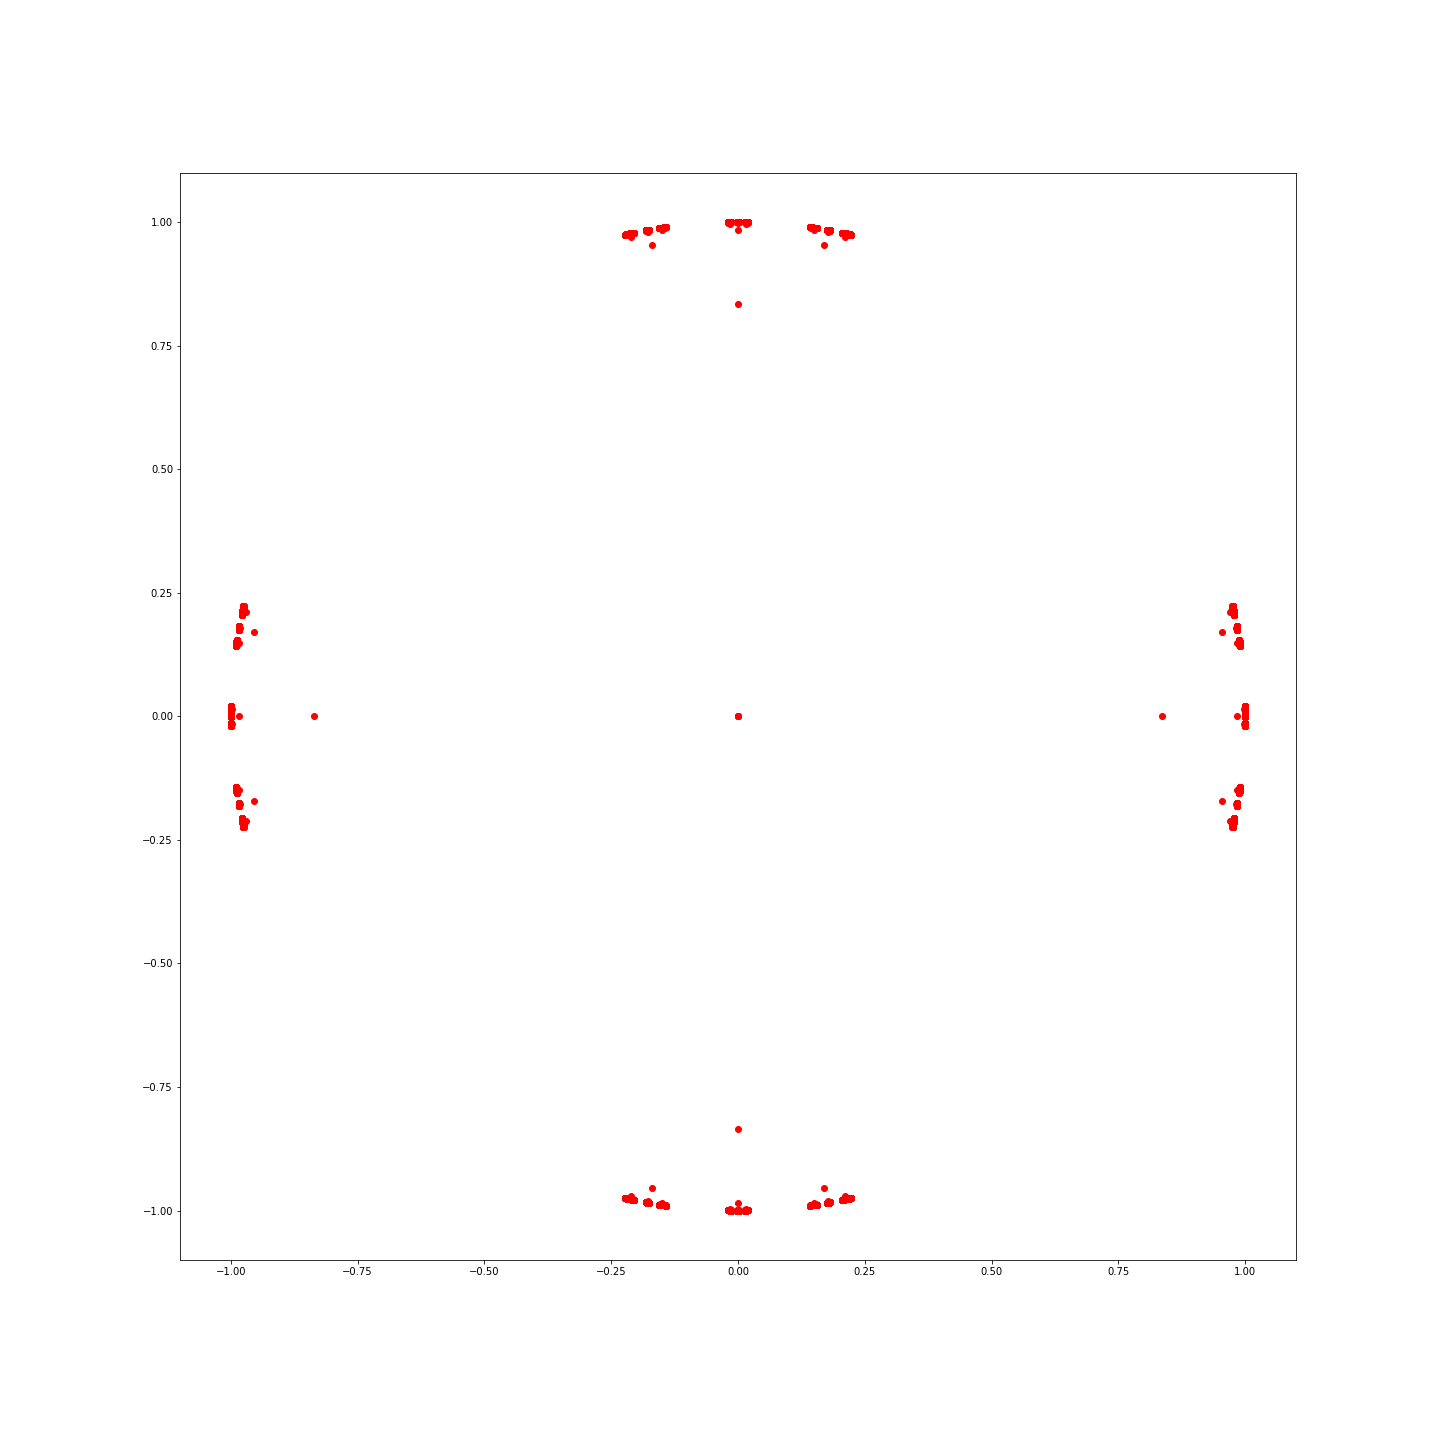
\includegraphics[width=0.8\textwidth]{Lambda=0.3,m=2,N=14.png}
\caption{$m=2$, $\Lambda=0.3$, $\theta\approx 33.398473447277695^{\circ}$, Level 14 ($N=14$).}
\end{figure}

\begin{figure}[H]
\centering
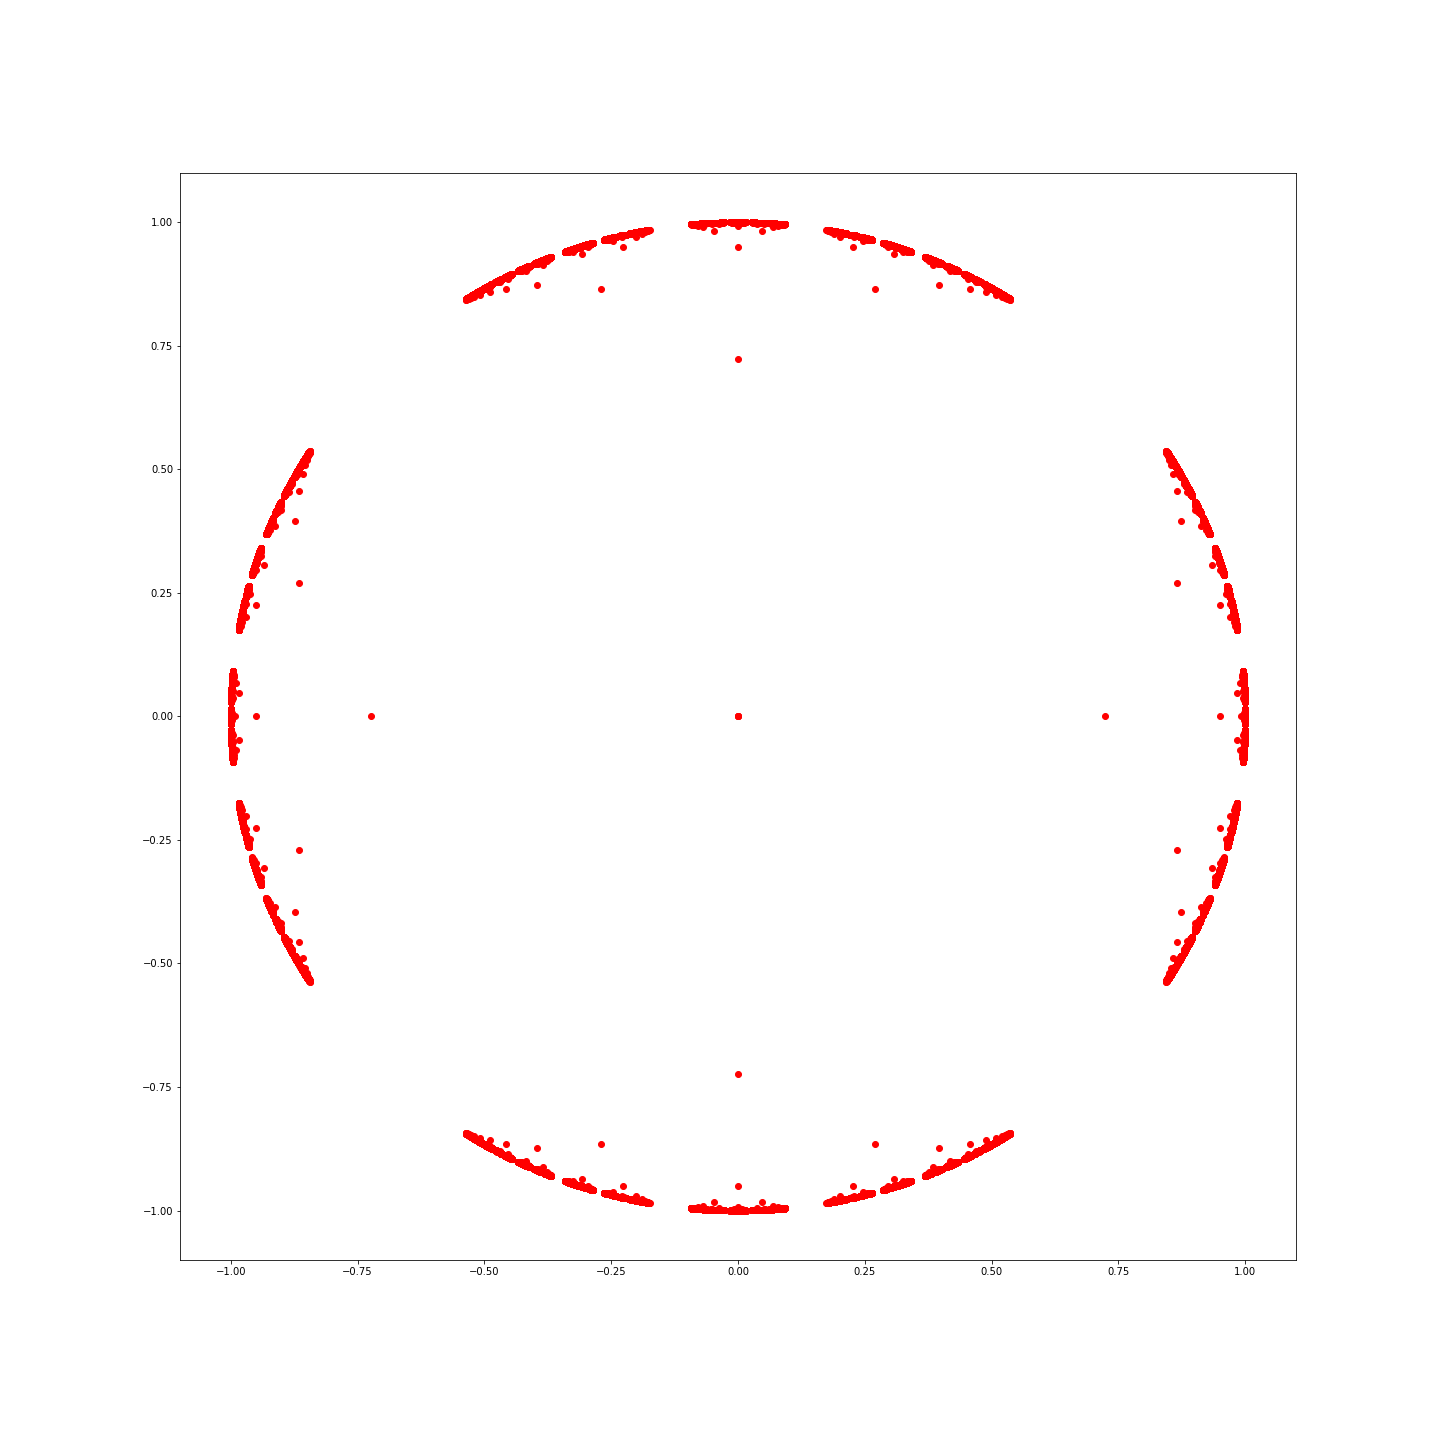
\includegraphics[width=0.8\textwidth]{Lambda=0.4,m=2,N=14.png}
\caption{$m=2$, $\Lambda=0.4$, $\theta\approx 43.602794482778144^{\circ}$, Level 14 ($N=14$).}
\end{figure}

\begin{figure}[H]
\centering
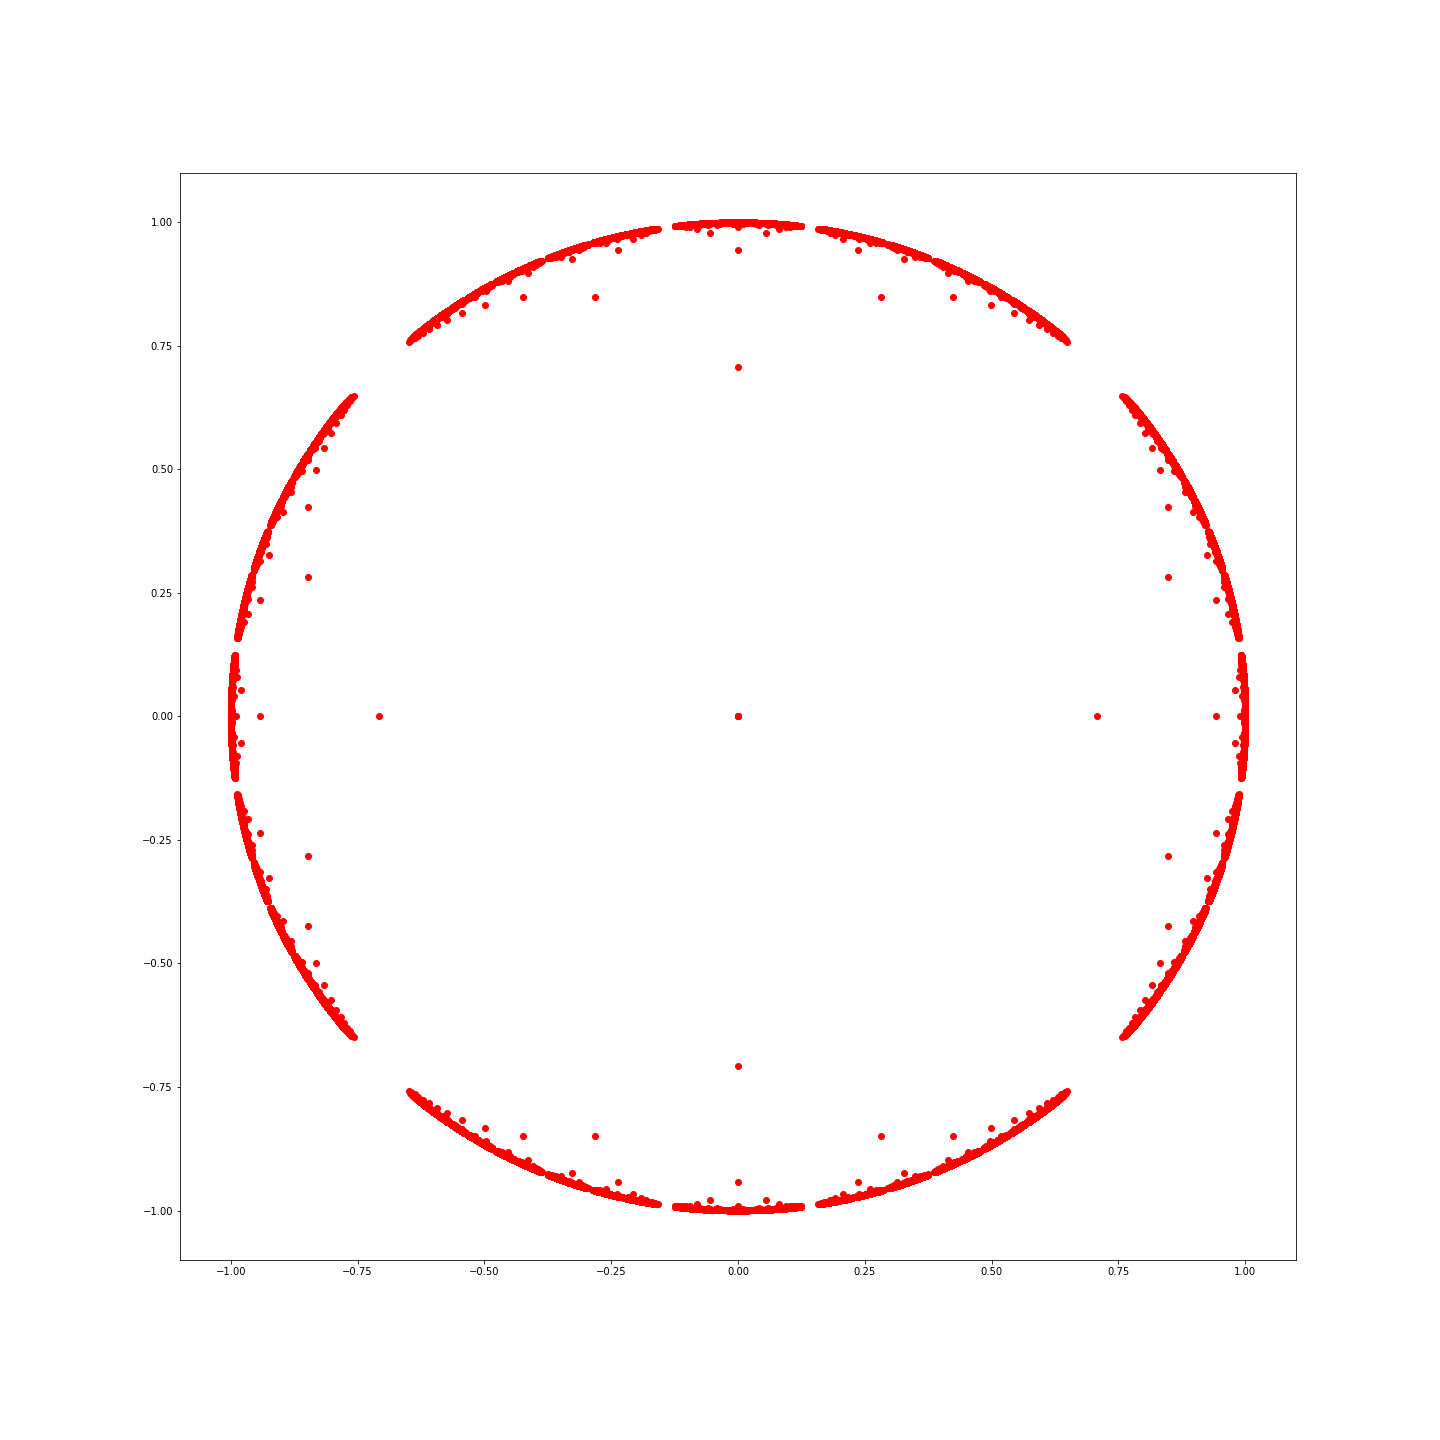
\includegraphics[width=0.8\textwidth]{Lambda=r,m=2,N=14.png}
\caption{$m=2$, $\Lambda\to\frac{\sqrt{2}}{2+\sqrt{2}}$, $\theta\to 45^{\circ}$, Level 14 ($N=14$).}
\end{figure}
 
Our computer system has a limit on the number of digits in a floating point number, but an irrational number $\frac{\sqrt{2}}{2+\sqrt{2}}$ has an endless number of digits after the decimal point.

That is, our computer system can only handle rational numbers, i.e., it can only employ rational numbers to approximate irrational numbers. As a result, in this picture, we have not obtained $\delta(G)=1$.

\begin{figure}[H]
\centering
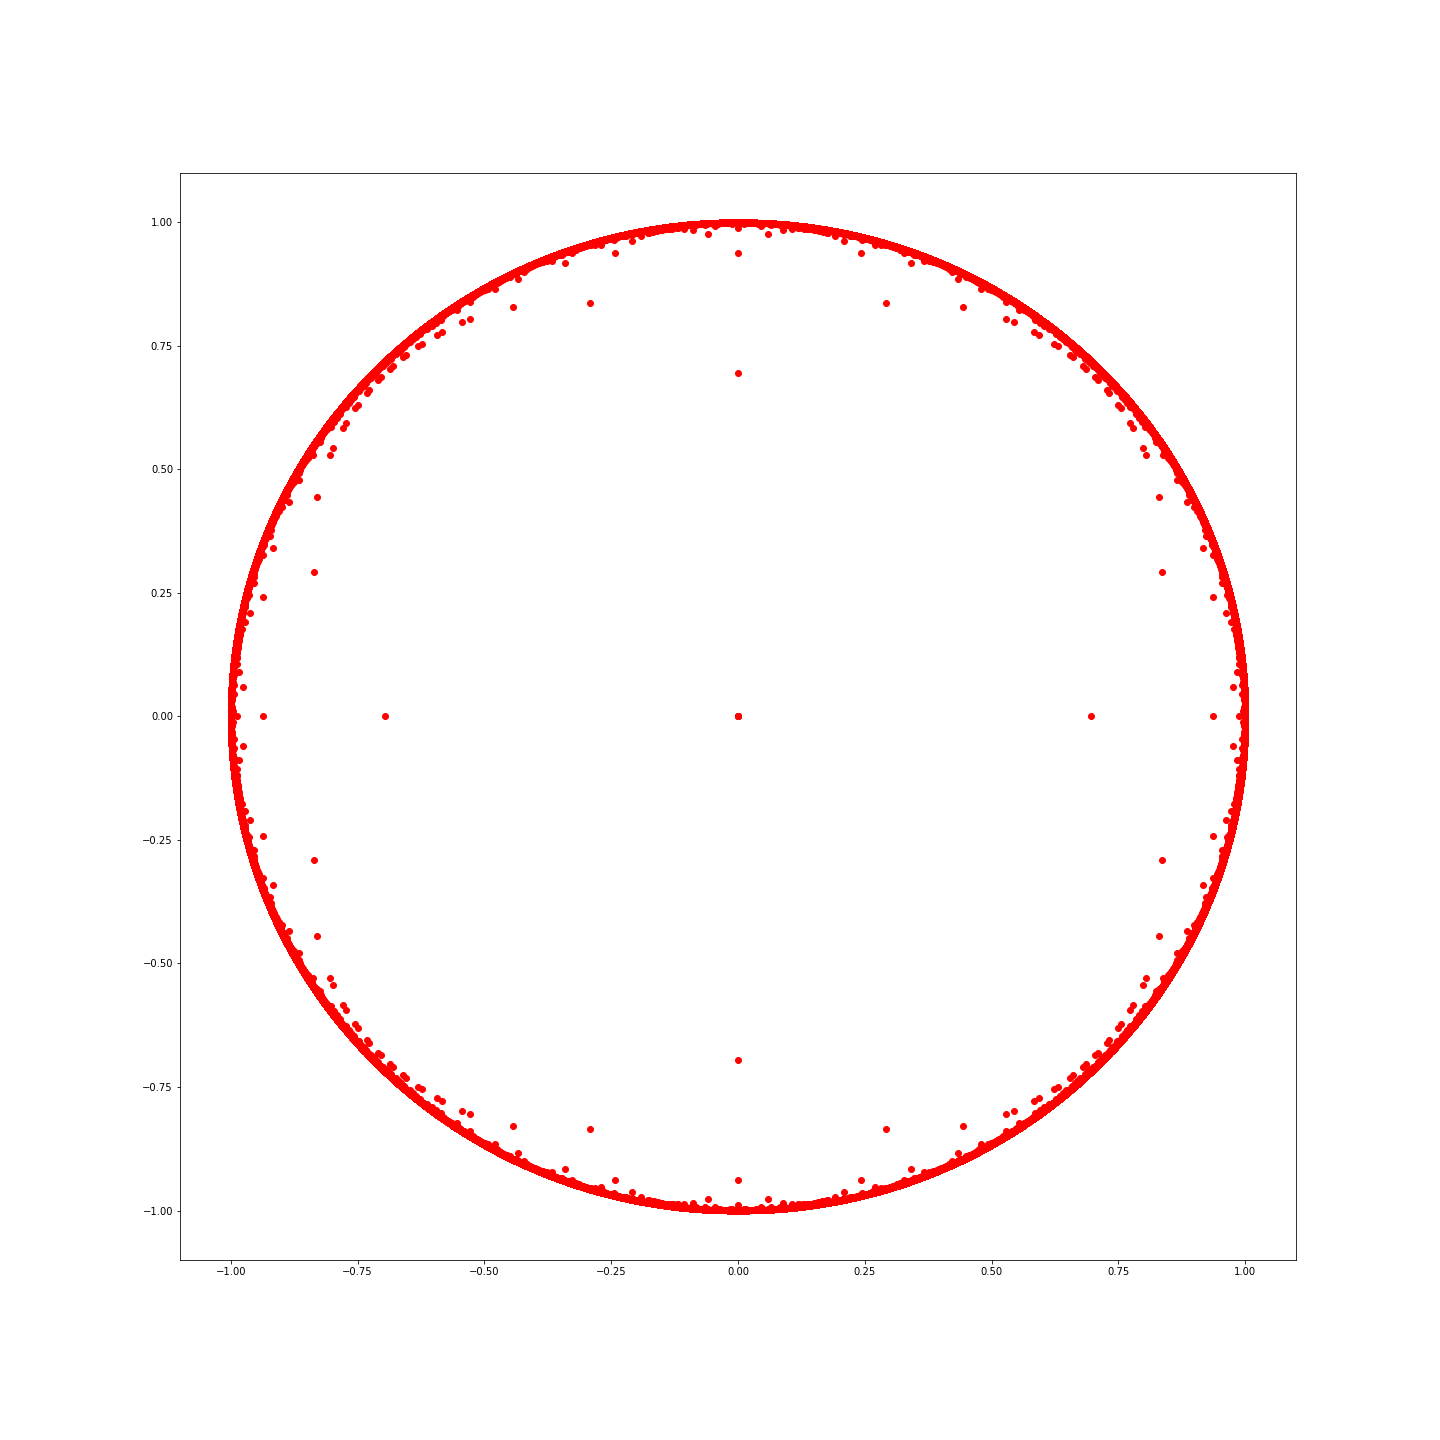
\includegraphics[width=0.8\textwidth]{Lambda=r+0.01,m=2,N=14.png}
\caption{$m=2$, $\Lambda=\frac{\sqrt{2}}{2+\sqrt{2}}+0.01$, $\theta\approx 45.9746105715017^{\circ}$, Level 14 ($N=14$).}
\end{figure}
To reach $\delta(G)=1$, we added a small number $0.01$ to let $\Lambda$ pass the number $\frac{\sqrt{2}}{2+\sqrt{2}}$, or equivalently to let $\theta$ passes $\frac{\pi}{2}$.

\begin{figure}[H]
\centering
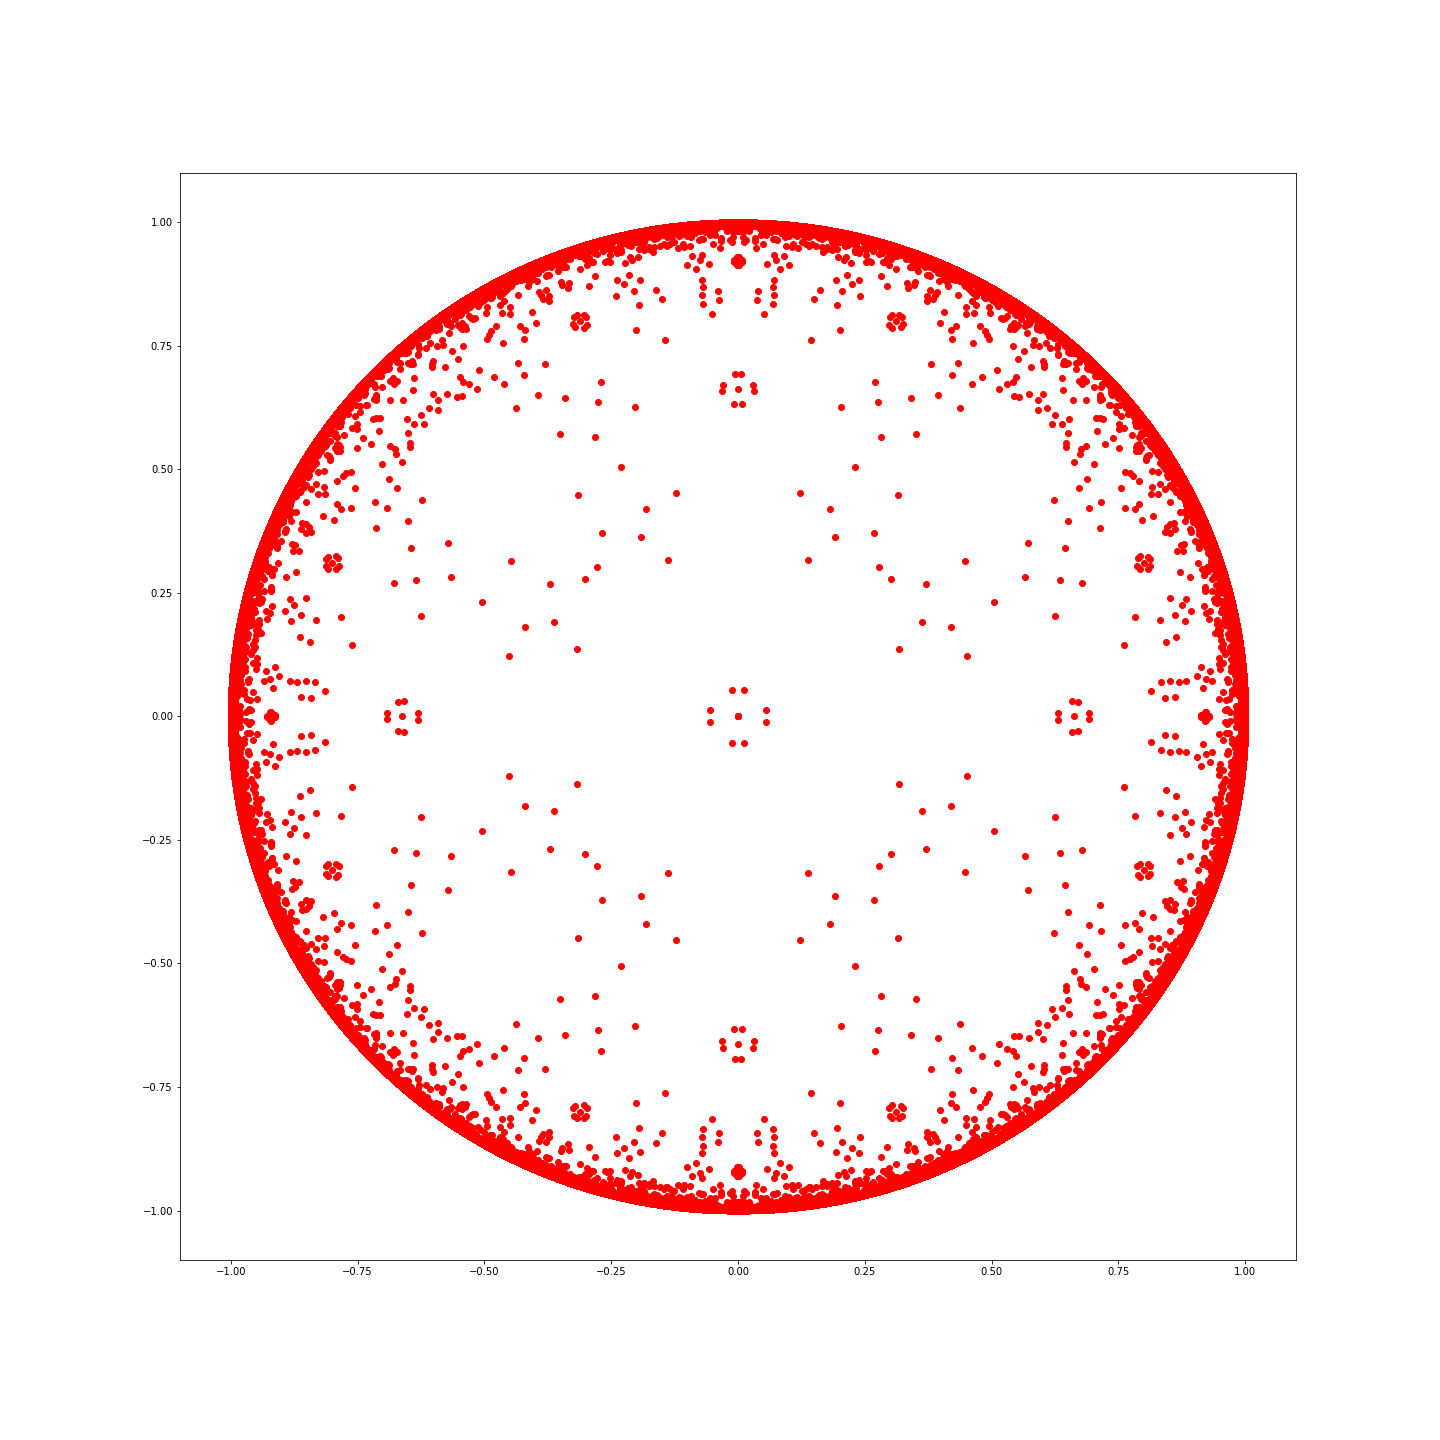
\includegraphics[width=0.8\textwidth]{Lambda=0.45,m=2,N=14.png}
\caption{$m=2$, $\Lambda=0.45$, $\frac{\theta}{2}\approx 48.455517824418166^{\circ}$, Level 14 ($N=14$).}
\end{figure}

\begin{figure}[H]
\centering
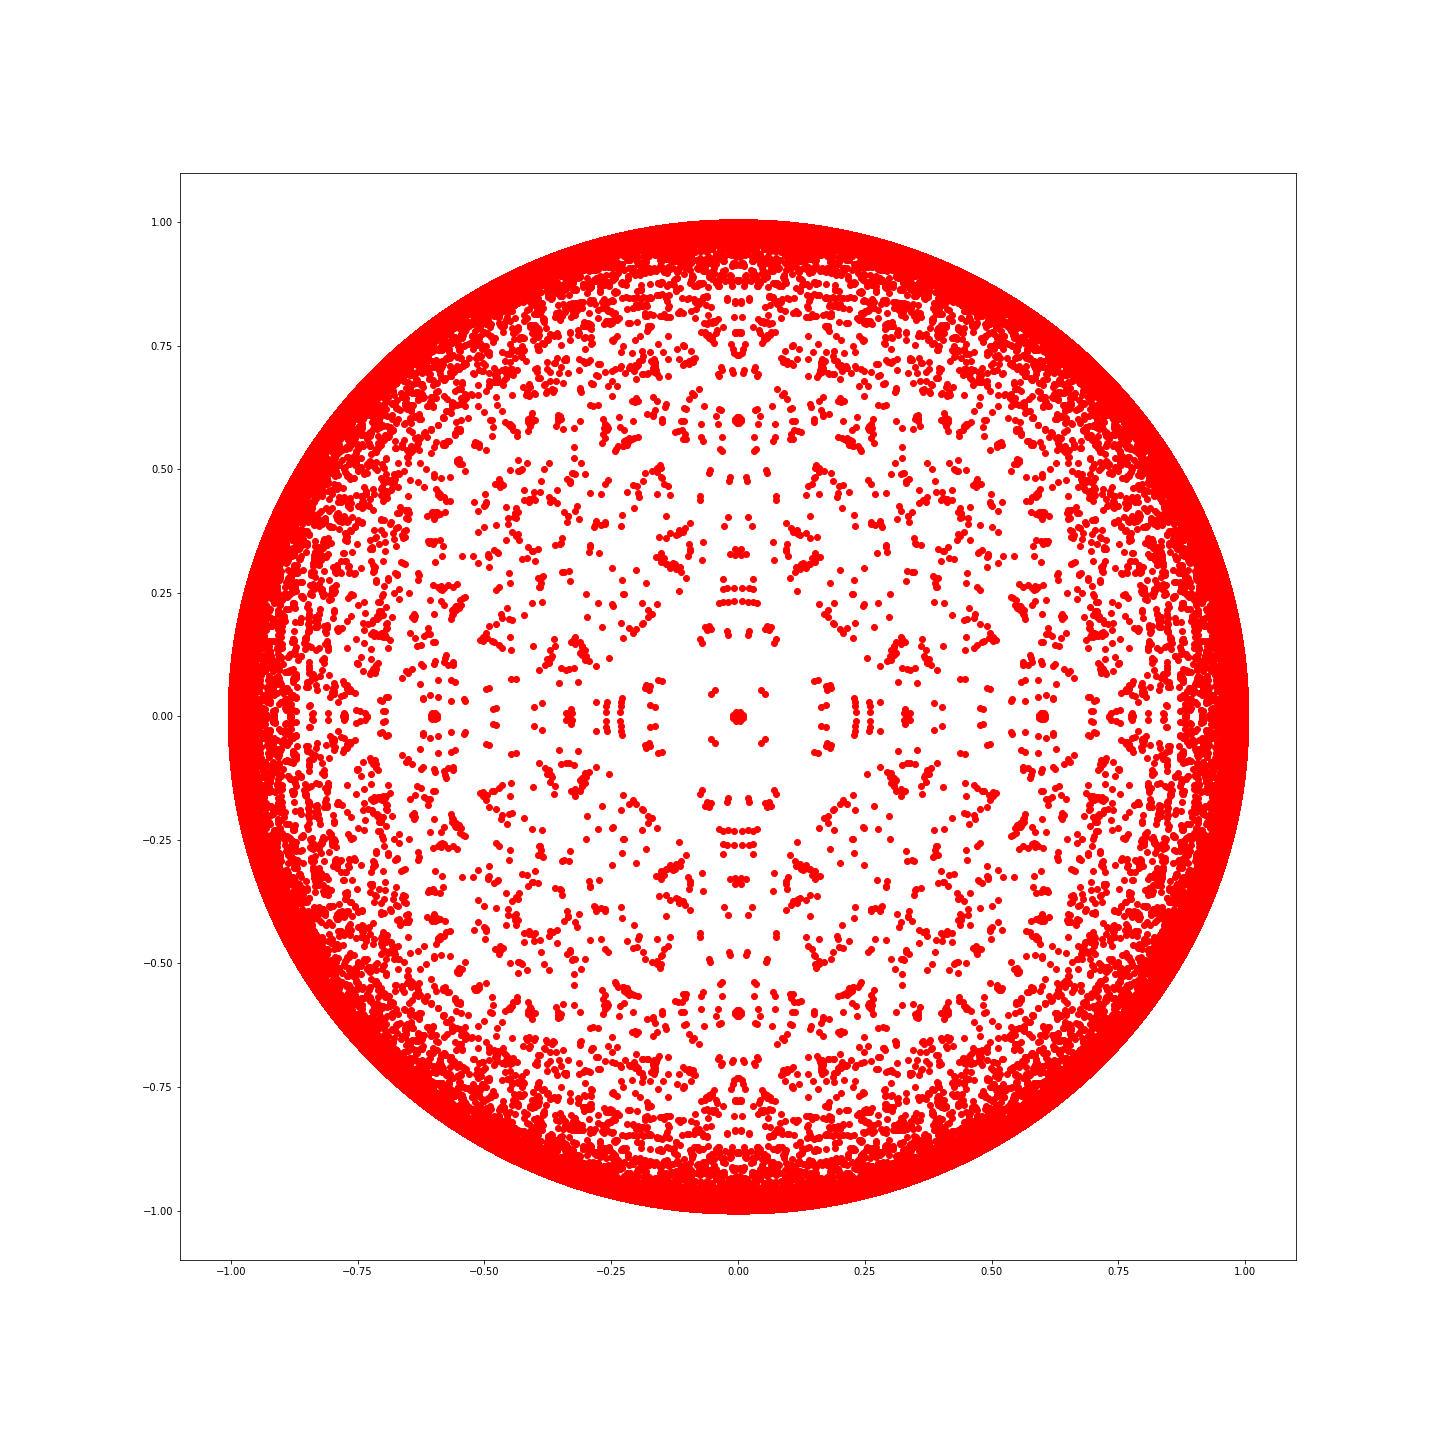
\includegraphics[width=0.8\textwidth]{Lambda=0.5,m=2,N=14.png}
\caption{$m=2$, $\Lambda=0.5$, $\theta\approx 53.13010858755201^\circ$, Level 14 ($N=14$).}
\end{figure}

\begin{figure}[H]
\centering
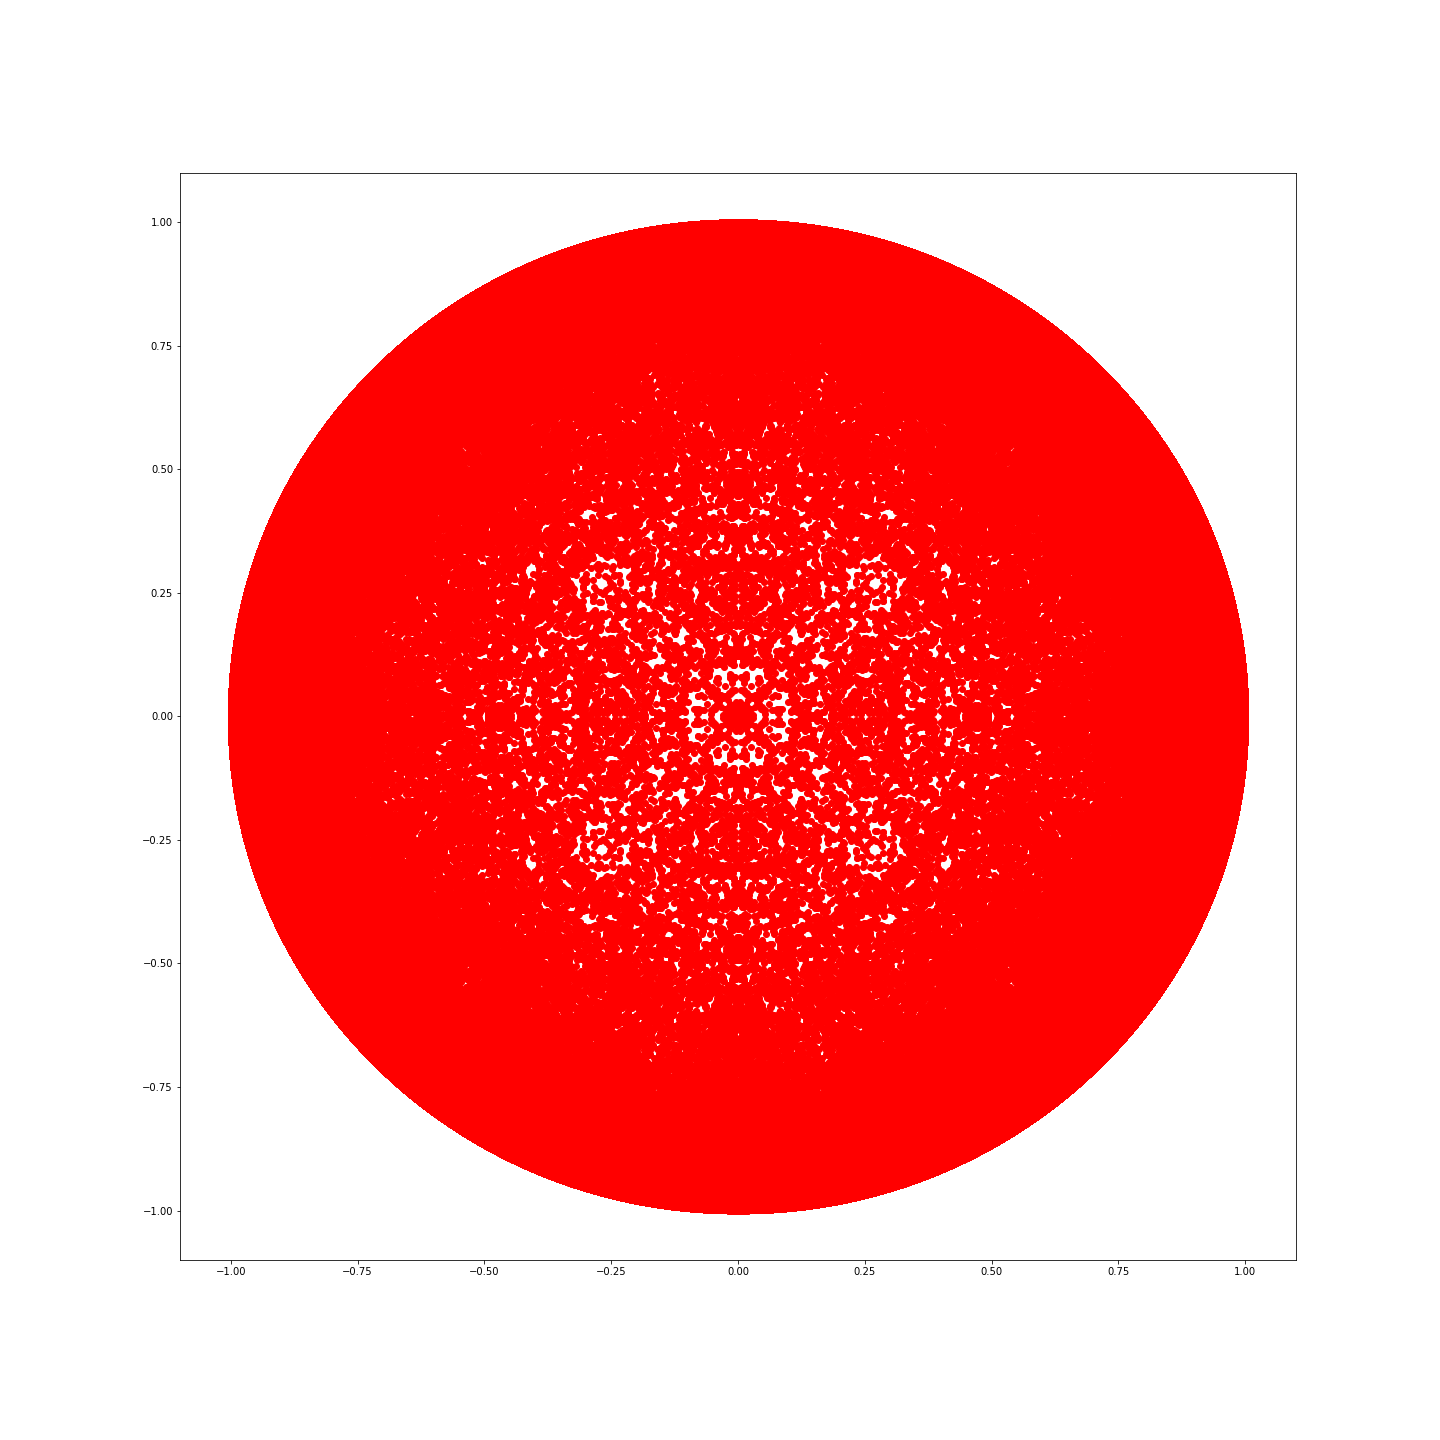
\includegraphics[width=0.8\textwidth]{Lambda=0.6,m=2,N=14.png}
\caption{$m=2$, $\Lambda=0.6$, $\theta\approx 61.927531757108724^\circ$, Level 14 ($N=14$).}
\end{figure}


To begin implementing McMullen's technique, we rotate the orbit by $\frac{\pi}{2}$ counter-clockwise by rotating the above $T$ operator and reassigning the result to the symbol $T$ in the following derivation.

In other words, we are going to find an alternative approach that instead of staring from $\mathbb{H}^2$, this time we directly start from $\mathbb{B}^2$ and use $\theta=\frac{\pi}{m}$ to parameterize $T$ instead of using $\Lambda$. 

Since on $\mathbb{B}^2$, to be an automorphism, we know $T$ must be in $\text{PSU}(1,1)$. Thus, assume
$$
T=\begin{pmatrix}
\alpha &  \overline{\gamma} \\
\gamma &  \overline{\alpha}
\end{pmatrix}.
$$

Then, for $0<\theta<\frac{\pi}{4}, \forall m\in\mathbb{Z}^+$, we can have
$$
T0=\cos\left(\frac{\theta}{2}\right).
$$
Thus
$$
\vert \gamma\vert^2=\vert \alpha\vert^2\cos^2\left(\frac{\theta}{2}\right).
$$
Since $T\in\text{PSU}(1,1)$, by definition of $\text{PSU}(1,1)$, we can obtain
$$
\vert \alpha\vert^2-\vert \gamma \vert^2=1.
$$
Hence,
$$
\vert \alpha\vert^2\sin^2\left(\frac{\theta}{2}\right)=1.
$$
That is
$$
\left(\sin^2\left(\frac{\theta}{2}\right) \right)^{-1}=\vert \alpha\vert^2.
$$
Without loss the generality, assume $\alpha=\left(\sin\left(\frac{\theta}{2}\right)\right)^{-1}$, and $\gamma=\cot\left(\frac{\theta}{2}\right)$ to satisfy the identity. 
Then we can define
$$
T:=\begin{pmatrix}
\frac{1}{\sin\left(\frac{\theta}{2}\right)} &  \cot\left(\frac{\theta}{2}\right) \\
\cot\left(\frac{\theta}{2}\right) &  \frac{1}{\sin\left(\frac{\theta}{2}\right)}
\end{pmatrix}.
$$
We can now utilize this revised definition of the operator $T$ to deduce the lemma and main theorem below.

%\begin{lemma}
%Let $I$ be the index corresponding to the boundary path, $r=\rho_{\mathbb{B}^2}\left(0,T0\right)$, and $I_n$ be the path at the level $n$. Then, 
%$$
%\lim\limits_{n\to\infty}\frac{x_{I_n}}{nr}<1.
%$$
%\end{lemma}
%\begin{proof}
%Recall lemma \ref{upper bound lemma}, we have
%$$
%\cosh\left( X_{I_n}\right) = \cosh\left( X_{I_{n-1}}\right)\cosh\left( 
%1-\tanh\left(X_{I_{n-1}}\tanh\left(r\right)\cos\left(\frac{\pi}{m}-\theta\right) \right)\right).
%$$
%Note that $0<\theta<\frac{\pi}{2m}$, so the factor
%$$
%1-\tanh\left( X_{I_{n-1}}\right) \tanh\left(r\right) \cos\left(\frac{\pi}{m}-\theta \right)
%\leq 1-\cos\left(\frac{\pi}{2m} \right):=C.
%$$
%Therefore, 
%$$
%\cosh\left(X_{I_n} \right)\leq C  \cosh\left( X_{I_{n-1}}\right)\cosh\left( r\right)
%$$
%$$
%\leq C^2\cosh\left(X_{I_{n-2}} \right)\cosh^2\left( r \right)\leq \cdots
%$$
%$$
%\leq C^n\cosh^n\left( r\right).
%$$
%Hence, 
%$$
%X_{I_{n}}\leq \cosh^{-1}\left( C^n\cosh^n\left(r\right)\right).
%$$
%Recall $\cosh^{-1}\left(y\right)=\ln\left(y+\sqrt{y^2-1} \right)$.

%Therefore, 
%$$
%X_{I_{n}}\leq \cosh^{-1}\left(C^n\cosh^n\left(r\right) \right)
%$$
%$$
%=\ln\left(C^n\cosh^n\left(r\right)+\sqrt{C^{2n}\cosh^{2n}\left( r\right)-1} \right)
%$$
%$$
%\leq \ln\left(2C^n\cosh^n\left( r\right) \right)
%$$
%$$
%=\ln\left(2\right)+n\ln\left(C\right)+n\ln\left(\cosh\left(r\right)\right).
%$$
%Hence, 
%$$
%\frac{X_{I_n}}{nr}\leq \frac{\ln\left(2\right)}{nr}+\frac{\ln\left(C\right)}{r}+\frac{\ln\left(C\right)}{r}.
%$$
%Take $n$ to infinity:
%$$
%\lim\limits_{n\to\infty}\frac{X_{I_{n}}}{nr}\leq \frac{\ln\left(\cosh\left(r\right)\right)}{r}+\frac{\ln\left(C\right)}{r}.
%$$
%If $C<1$, then $\ln\left(C\right)<0$, so we have
%$$
%\lim\limits_{n\to\infty}\frac{X_{I_{n}}}{nr}<\frac{\ln\left(\cosh\left(r\right)\right)}{r}
%$$
%$$
%=\frac{\ln\left(\frac{e^r+e^{-r}}{2}\right)}{r}<\frac{\ln\left(e^r\right)}{r}=1.
%$$
%\end{proof}



\begin{lemma}
Let $\Gamma=\left\langle T_1,\dots,T_m \right\rangle$ be well-distributed Schottky group, and let $$X_{I_n}=\rho_{\mathbb{B}^2}\left(0,T_I0 \right).$$ 

Consider the infinite index of a reduced word $I_n=(i_1,i_2,...,i_n,...)\in \mathcal{A}\times\mathcal{A}\cdots\times\mathcal{A}$, where each $\mathcal{A}=\left\lbrace 0,1,2,...,2m-1\right\rbrace$ is an alphabet, and $\mathcal{W}_n=\left\lbrace 
(i_1,i_2,...,i_n):i_j\in\mathcal{A}\right\rbrace$. 
Then from hyperbolic cosine law, we can have
$$
\cosh\left( X_{I_n}\right)=\cosh^n\left(r\right)\prod_{j=1}^{n-1}\left(1-\tanh\left(X_{I_{j+1}}\right)\tanh\left(r\right)\cos\left(\frac{i_{j+1}\pi}{m}-\theta_{I_j}\right)\right)
$$
\end{lemma}
\begin{proof}
After applying $T^{-1}_{I_n-1}$ and using the property of isometry, we can derive the following
$$
\angle\left(0,T_{I_{n-1}}0,T_{I_n}0\right)=\angle\left(T_{I_{n-2}},T_{I_{n-1}}0,T_{I_n}0\right)
-\angle\left(T_{I_{n-2}},T_{I_{n-1}}0,0\right)
$$
$$
=\angle\left(T^{-1}_{i_{n-1}},0,T_{i_n}0\right)-\angle\left(T^{-1}_{i_{n-1}}0,0,T^{-1}_{I_n-1}0\right)
$$
$$
=\frac{i_n\pi}{m}-\theta_{I_{n-1}}.
$$
Thus, the hyperbolic cosine law can be rewritten as follows
$$
\cosh\left( X_{I_n}\right)=\cosh\left( X_{I_{n-1}}\right)\cosh\left( r \right)
-\sinh\left( X_{I_{n-1}}\right)\sinh\left( r\right)\cos\left(\angle\left(0,T_{I_{n-1}}0,T_{I_n}0\right)\right)
$$
$$
=\cosh\left(X_{I_{n-1}}\right)\cosh\left( r\right)\left( 1- \tanh\left(X_{I_{n-1}}\right)\tanh\left(r\right)\cos\left( \frac{i_n\pi}{m}-\theta_{I_{n-1}}\right)\right)
$$
$$
=\cosh^2\left( r\right)\cosh\left(X_{I_{n-2}}\right)\left(1- \tanh\left(X_{I_{n-2}}\right)\tanh\left(r\right)\cos\left( \frac{i_{n-1}\pi}{m}-\theta_{I_{n-2}}\right)\right)
$$
$$
\times\left(1- \tanh\left(X_{I_{n-1}}\right)\tanh\left(r\right)\cos\left( \frac{i_n\pi}{m}-\theta_{I_{n-1}}\right)\right).
$$
By induction, we derived the following result
$$
\cosh\left( X_{I_n}\right)$$
$$=\cosh^{n-1}\left(r\right)\cosh\left(X_{I_{1}}\right)\prod_{j=1}^{n-1}\left( 1-\tanh\left(X_{I_{j+1}}\right)\tanh\left(r\right)\cos\left(\frac{i_{n-1}\pi}{m}-\theta_{I_{n-2}}\right)\right)
$$
$$
=\cosh^n\left(r\right)\prod_{j=1}^{n-1}\left(1-\tanh\left(X_{I_{j+1}}\right)\tanh\left(r\right)\cos\left(\frac{i_{j+1}\pi}{m}-\theta_{I_j}\right)\right)
$$
\end{proof}


\begin{definition}\label{PY}
Define the symbol for the previous lemma's outcome as follows.
$$
Y_{I_n}:=\cosh^n\left(r\right)\prod_{j=1}^{n-1}\left(1-\tanh\left(X_{I_{j+1}}\right)\tanh\left(r\right)\cos\left(\frac{i_{j+1}\pi}{m}-\theta_{I_j}\right)\right)
$$
and let
$$
P_n:=\sum_{T\in\mathcal{W}_n}\frac{1}{Y_{I_n}^t}.
$$
\end{definition}
\begin{lemma}
The Poincare\'{e} series can be rewritten using the above definition
$$
\mathcal{P}\left(\Gamma,t\right)\asymp \sum_{n=1}^\infty P_n.
$$
\end{lemma}
\begin{proof}
Recall $\rho_{\mathbb{B}^2}=\cosh^{-1}\left(X_{I_{n}}\right)= \ln\left(Y_{I_n}+\sqrt{Y_{I_n}^2-1}\right).$
$$
\mathcal{P}\left(\Gamma,t\right)=\sum_{T\in\Gamma}e^{-t\rho_{\mathbb{B}^2}\left(0,T0\right)}
\sum_{n=1}^\infty\sum_{T\in \mathcal{W}_n}e^{t\rho_{\mathbb{B}^2}\left(0,T0\right)}=\sum_{n=1}^\infty\sum_{T\in \mathcal{W}_n}\left(\frac{1}{Y_{I_n}+\sqrt{Y_{I_n}^2}-1} \right)^t
$$
$$
\asymp \sum_{n=1}^\infty\sum_{T\in \mathcal{W}_n}\frac{1}{Y_{I_n}^t}=\sum_{n=1}^\infty P_n.
$$
\end{proof}
\begin{theorem}
Suppose $\Gamma$ is a well-distributed Schottky group of order 2. Then, 
$$
\frac{\ln\left( 2\right)}{\ln\left(\cosh\left(r\right)\right)}\leq \delta\left(\Gamma\right)\leq
\min\left\lbrace \frac{\ln\left(4\right)}{\ln\left(\cosh\left(r\right)\right)},1\right\rbrace.
$$
\end{theorem}
\begin{proof}
Recall definition \ref{PY}, 
$$
Y_{I_n}=Y_{I_{n-1}i_n}=Y_{I_{n-1}} Y_{i_n}
$$
$$=\cosh\left(X_{I_{n-1}}\right)\cosh\left( r\right)\left( 1- \tanh\left(X_{I_{n-1}}\right)\tanh\left(r\right)\cos\left( \frac{i_n\pi}{m}-\theta_{I_{n-1}}\right)\right).
$$
Hence, 
\begin{small}
$$
Y_{I_{n+1}}=Y_{I_{n}} Y_{i_{n+1}}=\cosh\left(X_{I_{n}}\right)\cosh\left( r\right)\left( 1- \tanh\left(X_{I_{n}}\right)\tanh\left(r\right)\cos\left( \frac{i_{n+1}\pi}{m}-\theta_{I_{n}}\right)\right).
$$
\end{small}
Thus, for the $n+1$ term in $\mathcal{P}$, we can derive the following
$$
P_{n+1}=\sum_{T\in\mathcal{W}_{n+1}}\frac{1}{Y_{I_{n+1}}^t}=\sum_{T\in\mathcal{W}_n}\sum_{i_{n+1}=1}^{2m-1}\frac{1}{Y_{I_{n}i_{n+1}}^t}
$$


\begin{small}
$$=\sum_{T\in\mathcal{W}_n}\frac{1}{\left(\cosh\left(X_{I_{n}}\right)\right)^t}\frac{1}{\left(\cosh\left(r\right)\right)^t}\sum_{i_{n+1}=1}^{2m-1}\left(1-\tanh\left(X_{I_n}\right)\tanh\left(r\right)\cos\left(\frac{i_{n+1}\pi}{m}-\theta_{I_{n}}\right)\right)^{-t}.
$$
\end{small}
Recall Newton's generalized binomial theorem: Firstly, for $k\geq 1,k\in\mathbb{Z}$, we can have
$$
\binom{-t}{k}:=\frac{\left(-t-0\right)\left(-t-1\right)\cdots \left(-t-\left(k-1\right)\right)}{k!}
$$
$$
=\frac{t\left(t+1\right)\cdots\left(t+\left(k-1\right)\right)}{k!}\left(-1\right)^k, \forall k \in\mathbb{Z}^{+},
$$
and secondly for $k=0$, we can obtain
$$
\binom{-t}{0}:=1.
$$
Hence, 
$$
\left(x+y \right)^{-t}=\sum_{k=0}^\infty \binom{-t}{k} x^{-t-k}y^k.
$$
Now, let $x=1$, and replace $y$ with $-y$.
$$
\left(1-y \right)^{-t}=\sum_{k=0}^\infty \binom{-t}{k} \left(-1\right)^k y^k
$$
$$
=\sum_{k=0}^\infty \frac{t\left(t+1\right)\cdots\left(t+\left(k-1\right)\right)}{k!} \left(-1\right)^{2k} y^k
$$
$$ = \sum_{k=0}^\infty \frac{t\left(t+1\right)\cdots\left(t+\left(k-1\right)\right)}{k!}   y^k
$$
$$
=1+ty+\sum_{k=2}^\infty \frac{t\left(t+1\right)\cdots\left(t+\left(k-1\right)\right)}{k!} y^k.
$$

Thus, 
$$
\sum_{i_{n+1}=1}^{2m-1}\left(1-\tanh\left(X_{I_n}\right)\tanh\left(r\right)\cos\left(\frac{i_{n+1}\pi}{m}-\theta_{I_{n}}\right)\right)^{-t}
$$
$$
=\sum_{i_{n+1}=1}^{2m-1}\left( 1+t\tanh\left( X_{I_n}\right)\tanh\left(r \right)\cos \left(\frac{i_{n+1} \pi}{m}-\theta_{I_n} \right)\right.
$$
$$
\left.
+\sum_{k=2}^{\infty}\frac{t\left(t+1\right)\cdots\left(t+\left(k-1\right)\right)}{k!}\tanh^k\left(X_{I_n}\right)\tanh^k\left(r\right)\cos^k\left(\frac{i_{n+1}\pi}{m}-\theta_{I_{n}}\right)
\right)
$$
$$
=2m-1+t\tanh\left(X_{I_n} \right)\tanh\left(r\right)\left(\sum_{i_{n+1}=1}^{2m-1}\cos\left(\frac{i_{n+1}\pi}{m}-\theta_{I_n}\right) \right)
$$
$$
+\sum_{k=2}^{\infty}\frac{t\left(t+1\right)\cdots\left(t+\left(k-1\right)\right)}{k!}
\left(\sum_{i_{n+1}=1}^{2m-1} 
\tanh^k\left(X_{I_n}\right)\tanh^k\left(r\right)\cos^k\left(\frac{i_{n+1}\pi}{m}-\theta_{I_{n}}\right)
\right)
$$

Let $m=2$. Hence,
$$
\sum_{i_{n+1}=1}^{3} \cos^k\left(\frac{i_{n+1} \pi}{2}-\theta_{I_n} \right)=\cos^k\left(\frac{\pi}{2}-\theta_{I_n}\right)+\cos^k\left(\pi-\theta_{I_n}\right)+\cos^k\left(\frac{3 \pi}{2}-\theta_{I_n}\right)
$$
$$
=\begin{cases} 
      -\cos^k\left(\theta_{I_n}\right) & k \text{ is odd }  \\
      2\sin^k\left(\theta_{I_n}\right)+\cos^k\left(\theta_{I_n}\right) & k\text{ is even.} 
   \end{cases}
$$
The estimation becomes the following
$$
\sum_{i_{n+1}=1}^{3}\left(1-\tanh\left(X_{I_n}\right)\tanh\left(r\right)\cos\left(\frac{i_{n+1}\pi}{2}-\theta_{I_{n}}\right)\right)^{-t}
$$
$$
=3-t\tanh\left(X_{I_n} \right)\tanh\left(r\right)\cos\left(\theta_{I_n}\right)
$$
$$
-\sum_{l=1}^{\infty}\frac{t\left(t+1\right)\cdots\left(t+\left((2l+1)-1\right)\right)}{\left(2l+1\right)!}
\left( 
\tanh^{2l+1}\left(X_{I_n}\right)\tanh^{2l+1}\left(r\right)\cos^{2l+1}\left(\theta_{I_n}\right)
\right)
$$
$$
+\sum_{l=1}^{\infty}\frac{t\left(t+1\right)\cdots\left(t+\left((2l)-1\right)\right)}{\left(2l\right)!}
\left( 
\tanh^{2l}\left(X_{I_n}\right)\tanh^{2l}\left(r\right)\left(2\sin^{2l}\left(\theta_{I_n}\right)+\cos^{2l}\left(\theta_{I_n}\right)\right)
\right)
$$
$$
=3-t\tanh\left(X_{I_n} \right)\tanh\left(r\right)\cos\left(\theta_{I_n}\right)
$$
$$
+\sum_{l=2}^{\infty}(-1)^l\frac{t\left(t+1\right)\cdots\left(t+\left((l)-1\right)\right)}{\left(l\right)!}
\left( 
\tanh^{2l+1}\left(X_{I_n}\right)\tanh^{2l+1}\left(r\right)\cos^{l}\left(\theta_{I_n}\right)
\right)
$$
$$
+\sum_{l=1}^{\infty}\frac{t\left(t+1\right)\cdots\left(t+\left((2l)-1\right)\right)}{\left(2l\right)!}
\left( 
\tanh^{2l}\left(X_{I_n}\right)\tanh^{2l}\left(r\right)2\sin^{2l}\left(\theta_{I_n}\right)
\right).
$$
Notice $0<\theta_{I_n}<\frac{\pi}{4}$, $0<t<1,$
$$
\sum_{l=1}^{\infty}\frac{t\left(t+1\right)\cdots\left(t+\left((2l)-1\right)\right)}{\left(2l\right)!}
\left( 
\tanh^{2l}\left(X_{I_n}\right)\tanh^{2l}\left(r\right)2\sin^{2l}\left(\theta_{I_n}\right)
\right)
$$
$$
\leq \sum_{l=1}^\infty \frac{1\cdot 2\cdot \cdots \cdot 2l}{(2l)!}2\cdot \frac{1}{\sqrt{2}^{2k}}=2\cdot \sum_{k=2}^\infty\frac{1}{2^k}=1.
$$
Hence, 
$$
\sum_{i_{n+1}=1}^{3}\left(1-\tanh\left(X_{I_n}\right)\tanh\left(r\right)\cos\left(\frac{i_{n+1}\pi}{2}-\theta_{I_{n}}\right)\right)^{-t}\leq 3+
$$
$$
\left(1+\sum_{l=2}^{\infty}(-1)^l\frac{t\left(t+1\right)\cdots\left(t+\left((l)-1\right)\right)}{\left(l\right)!}
\left( 
\tanh^{2l+1}\left(X_{I_n}\right)\tanh^{2l+1}\left(r\right)\cos^{l}\left(\theta_{I_n}\right)
\right)
\right)
$$
$$
=3+\left(1+\tanh\left(X_{I_n}\right)\tanh\left(r\right)\cos\left(\theta_{I_n}\right)\right)^{-t}.
$$
Since
$$
\left(1+y\right)^{-t}=1+\sum_{k=1}^\infty\frac{(-t)(-t-1)\cdots (-t-(k-1))}{k!}y^k
$$
$$
=1+\sum_{k=1}^\infty\frac{t(t+1)\cdots(t+k-1)(-1)^k y^k}{k!},
$$ 
and $\frac{1}{\left(1+\tanh\left(X_{I_n}\right)\tanh\left(r\right)\cos\left(\theta_{I_n}\right)\right)^t}\leq 1$,
$$
P_{n+1}\leq \sum_{T\in\mathcal{W}_n}\frac{1}{\left(\cosh\left(X_{I_n}\right)\right)^t\left(\cosh\left(r\right)\right)^t}\left(3+\frac{1}{\left(1+\tanh\left(X_{I_n}\right)\tanh\left(r\right)\cos\left(\theta_{I_n}\right)\right)^t}\right)
$$
$$
\leq \frac{4}{\cosh^t\left(r\right)}P_{n}.
$$


Thus,
$$
\mathcal{P}\left(\Gamma,t\right)\leq P_1\sum_{n=1}^\infty\left(\frac{4}{(\cosh\left(r\right))^t}\right)^n.
$$
This implies that
$$
\delta\left(\Gamma\right)\leq \frac{\ln\left(4\right)}{\ln\left(\cosh\left(r\right)\right)}.
$$
To obtain a lower bound, recall
$$
\sum_{i_{n+1}=1}^{3}\left(1-\tanh\left(X_{I_n}\right)\tanh\left(r\right)\cos\left(\frac{i_{n+1}\pi}{2}-\theta_{I_{n}}\right)\right)^{-t}
$$
$$
=3-t\tanh\left(X_{I_n} \right)\tanh\left(r\right)\cos\left(\theta_{I_n}\right)
$$
$$
+\sum_{l=2}^{\infty}(-1)^l\frac{t\left(t+1\right)\cdots\left(t+\left((l)-1\right)\right)}{\left(l\right)!}
\left( 
\tanh^{2l+1}\left(X_{I_n}\right)\tanh^{2l+1}\left(r\right)\cos^{l}\left(\theta_{I_n}\right)
\right)
$$
$$
+\sum_{l=1}^{\infty}\frac{t\left(t+1\right)\cdots\left(t+\left((2l)-1\right)\right)}{\left(2l\right)!}
\left( 
\tanh^{2l}\left(X_{I_n}\right)\tanh^{2l}\left(r\right)2\sin^{2l}\left(\theta_{I_n}\right)
\right)
$$
$$
\geq 2+\frac{1}{\left(1+\tanh\left(X_{I_n}\right)\tanh\left(r\right)\cos\left(\theta_{I_n}\right)\right)^t}.
$$
Implying that
$$
P_{n+1}\geq \frac{2}{\cosh^t\left(r\right)}P_n,
$$
and hence
$$
\mathcal{P}\left(\Gamma,t\right) \geq P_1\sum_{n=1}^\infty\left(\frac{2}{\cosh^t\left(r\right)}\right)^n.
$$
Therefore, 
$$
\delta\left(\Gamma\right)\geq \frac{\ln\left(2\right)}{\ln\left(\cosh\left(r\right)\right)}.
$$
\end{proof}
The above bounds can be further sharpen into the following:
\begin{theorem}\label{main thm 11}
Suppose $\Gamma$ is a well-distributed Schottky group of order 2. Then, 
$$
\frac{\ln\left( 2+\frac{1}{1+2\sqrt{2}}\right)}{\ln\left(\cosh\left(r\right)\right)}\leq \delta\left(\Gamma\right)\leq
\min\left\lbrace \frac{\ln\left(4-\frac{2}{1+2\sqrt{2}}\right)}{\ln\left(\cosh\left(r\right)\right)},1\right\rbrace.
$$
\end{theorem}
\begin{proof}
Firstly, since $\tanh\left(X_{I_n}\right)\geq \tanh\left(r\right)$, and $0<\alpha\leq\frac{\pi}{4}$. Thus,
$$
\tanh\left(X_{I_n}\right)\tanh\left(r\right)\cos\left(\theta_{I_n}\right)>\tanh^2\left(r\right)\cos\left(\theta_{I_n}\right)>\frac{1}{\sqrt{2}}\tanh^2\left(r\right).
$$
Secondly, the choice of the operator $T$ is as follows:
$$
T=\begin{pmatrix}
\frac{1}{\sin\left(\frac{\alpha}{2}\right)} &  \cot\left(\frac{\alpha}{2}\right) \\
\cot\left(\frac{\alpha}{2}\right) &  \frac{1}{\sin\left(\frac{\alpha}{2}\right)}
\end{pmatrix}.
$$
Hence, 
$$\vert T0\vert=\cos\left(\frac{\alpha}{2}\right).$$
Then, 
$$
\tanh\left(r\right)=\tanh\left(\ln\left(\frac{1+\vert T0\vert}{1-\vert T0\vert}\right)\right)=\frac{2}{\cos\left(\frac{\alpha}{2}\right)}.
$$

Therefore,
$$
\frac{1}{\left(1+\tanh\left(X_{I_n}\right)\tanh\left(r\right)\cos\left(\theta_{I_n}\right)\right)^t}\geq \frac{1}{\left(1+2\sqrt{2}\right)^t}\geq \frac{1}{1+2\sqrt{2}}.
$$
On the other hand, since 
$$
t\tanh\left(X_{I_n} \right)\tanh\left(r\right)\cos\left(\theta_{I_n}\right)\leq \frac{2}{\cos\left(\frac{\alpha}{2}\right)},
$$
and recall that 
$$
\sum_{i_{n+1}=1}^{3}\left(1-\tanh\left(X_{I_n}\right)\tanh\left(r\right)\cos\left(\frac{i_{n+1}\pi}{2}-\theta_{I_{n}}\right)\right)^{-t}
$$
$$
=3-t\tanh\left(X_{I_n} \right)\tanh\left(r\right)\cos\left(\theta_{I_n}\right)
$$
\begin{small}
$$
-\sum_{l=1}^{\infty}\frac{t\left(t+1\right)\cdots\left(t+\left((2l+1)-1\right)\right)}{\left(2l+1\right)!}
\left( 
\tanh^{2l+1}\left(X_{I_n}\right)\tanh^{2l+1}\left(r\right)\cos^{2l+1}\left(\theta_{I_n}\right)
\right)
$$
$$
+\sum_{l=1}^{\infty}\frac{t\left(t+1\right)\cdots\left(t+\left((2l)-1\right)\right)}{\left(2l\right)!}
\left( 
\tanh^{2l}\left(X_{I_n}\right)\tanh^{2l}\left(r\right)\left(2\sin^{2l}\left(\theta_{I_n}\right)+\cos^{2l}\left(\theta_{I_n}\right)\right)
\right).
$$
\end{small}
Instead of taking the minimum of the term $-t\tanh\left(X_{I_n} \right)\tanh\left(r\right)\cos\left(\theta_{I_n}\right)$ by zero, now we use a sharper bound $\frac{2}{\cos\left(\frac{\alpha}{2}\right)}$, and this implies 
$$
\sum_{i_{n+1}=1}^{3}\left(1-\tanh\left(X_{I_n}\right)\tanh\left(r\right)\cos\left(\frac{i_{n+1}\pi}{2}-\theta_{I_{n}}\right)\right)^{-t}
$$
$$
\leq 3-\left(\frac{2}{\cos\left(\frac{\alpha}{2}\right)}\right)+\frac{1}{\left(
1+\frac{2}{\cos\left(\frac{\alpha}{2}\right)}
\right)^t}.
$$
The proof is complete after inserting the aforementioned revised bounds into the prior theorem's proof.
\end{proof}



Based on the above theorems, we conjecture
$$
\delta\left(\Gamma\right)=\frac{\ln\left(3\right)}{\ln\left(\cosh\left(r\right)\right)}.
$$
To see why this conjecture may be true, we consider $\alpha=\frac{\pi}{4}$. Then, 
$$
T0=\cos\left(\frac{\pi}{4}\right),
$$
and 
$$
r=\ln\left(\frac{\sqrt{2}+1}{\sqrt{2}-1}\right).
$$
Then, 
$$
\cosh\left(r\right)=\frac{e^r+e^{-r}}{2}=\frac{\frac{\sqrt{2}+1}{\sqrt{2}-1}+\frac{\sqrt{2}-1}{\sqrt{2}+1}}{2}=3.
$$
Therefore,
$$
\frac{\ln\left(3\right)}{\ln\left(\cosh\left(r\right)\right)}=1.
$$

Furthermore, towards the conclusion of the next chapter, this conjecture was analytically tested using an approximation based on McMullen's technique.


\chapter{McMullen's Algorithm}

The purpose of this chapter is to introduce McMullen's algorithm, which is by far the most accurate approach for numerically approximating the Hausdorff dimension of limit sets of Schottky groups. However, the original source code used to get the findings was never published\cite{mcmullen1998hausdorff}, therefore we re-implemented the algorithm in C and reproduced the results to check that our knowledge and implementation of Patterson-Sullivan theory and McMullen's algorithm were valid. Furthermore, based on McMullen's derivation, we obtained an approximation for small angles that corresponds to the result produced by our conjecture, which is also included in this chapter.

In 1998, McMullen\cite{mcmullen1998hausdorff} proposed an algorithm for estimating the Hausdorff dimension of a set associated with a conformal dynamical system (as Julia sets or limit set of a geometrically finite Kleinian groups). The dimension of the related Patterson-Sullivan measures coincides with the Hausdorff dimension of its limit set, and McMullen's approach works to estimate the Hausdorff dimension of the Schottky group limit set.

In \cite{mcmullen1998hausdorff}, some definitions were used for proving a theorem that supports McMullen's algorithm that were used in our set-up of well-distributed group:
\begin{definition}
\textit{A $G-$invariant density of dimension $\delta$} is a finite positive measure $\mu$ on $\mathbb{S}^1$ such that
$$
\mu\left(T\left(E\right)\right)=\int_{E}\vert T'(z) \vert^\delta d\mu
$$
whenever $T\vert_{E}$ is injective, $E\subset \partial \mathbb{B}^2\cup \mathbb{B}^2$ is a Borel set and $T\in G$.
\end{definition}

To describe the theorem and McMullen's algorithm, we need to define Markov partitions and their refinements.
\begin{definition}
Let $G$ be a Schottky group. \textit{A Markov partition} for $(G,\mu)$ is a nonempty collection $\mathcal{I}\left\langle (I_i,T_i) \right\rangle$ of connected compact intervals $I_i\subset \mathbb{S}^1$, $T_i\in G$ meet the following requirements:
\begin{itemize}
\item $T_i(I_i)\supset \cup_{i\mapsto j}I_j$, where the relation $i\mapsto j$ means $\mu\left(T_i(I_i)\cap I_j \right)>0$.
\item $T_i$ is a homeomorphism on a neighborhood of $I_i\cap T_i^{-1}(I_j)$, when $i\mapsto j$;
\item $\mu(I_i)>0$;
\item $\mu(I_i\cap I_j)=0$ if $i\neq j$; and
\item $\mu(T_i(I_i))\mu(\cup_{i\mapsto j}I_j)=\sum_{i\mapsto j}\mu (I_j).$
\end{itemize}
\end{definition}
\begin{definition}
\textit{A refinement} of a Markov partition $\mathcal{I}$ is a new Markov partition:
$$
\mathcal{R}(\mathcal{I})=\left\langle (R_{ij},T_i):i\mapsto j \right\rangle
$$ 
where $R_{ij}:=T_i^{-1}(I_j)\cap I_i$.
\end{definition}


\begin{definition}
If there exists a smooth conformal metric $\rho$ on $\mathbb{S}^1$ and a constant $\nu$ such that
$$
\vert T'_{i}(x)\vert_\rho>\nu>1,
$$
whenever $x\in I_i$ and $T_i(x)\in I_j$ for some $j$, then the Markov partition is \textit{expanding}.
\end{definition}

To outline the algorithm's five primary phases for computing the dimension $\delta$ of the density $\mu$, firstly, let us consider a Schottky group $G$, a Markov partition $\mathcal{I}=\left\langle (I_i,T_i)\right\rangle$, and sample points $x_i\in I_i$ (in our implementation, the midpoint of each interval $I_i$ was chosen to be $x_i$). The algorithm computes a sequence of estimates from $\alpha\left( \mathcal{R}^n(I)\right)$ to $\delta$ and then proceeds as follows:
\begin{itemize}
\item Step 1. For each $i\mapsto j$, solve for $y_{ij}\in I_i$ such that $T_i(y_{ij})=x_j$.
\item Step 2. Compute the transition matrix
$$
T_{ij}=\begin{cases} 
      \vert T'_i(y_{ij}) \vert^{-1} & \text{if }i\mapsto j, \\
      0 & \text{otherwise.}
   \end{cases}
$$
\item Step 3. Find $\alpha(\mathcal{I})\geq 0$ such that the spectral radius (the greatest eigenvalue of the matrix $T_{ij}^\delta$, i.e. the transition matrix raised to the power $\alpha$) equals unity. 
\item Step 4. Return $\alpha(\mathcal{I})$ as an approximation to $\delta$ of this iteration.
\item Step 5. Refine the Markov partition, define new sample points $x_{ij}=y_{ij}\in R_{ij}$, and start afresh from Step 1.
\end{itemize}
The algorithm is supported by the following theorem\cite{mcmullen1998hausdorff}:
\begin{theorem}[McMullen]
Let $\mathcal{I}$ be an expanding Markov partition for a Schottky group $G$ with invariant density $\mu$ of dimension $\delta$. Then
$$
\alpha(\mathcal{R}^n(\mathcal{I}))\to \delta
$$
as $n\to \infty$. 
\end{theorem}
Hence, the dimension of the conformal measure, $\delta$, is approximated by the power $\alpha$.

The worst case scenario of this theorem could be the case when angle $\theta\to \frac{2\pi}{3}$ in the symmetric pairs of pants example in \cite{mcmullen1998hausdorff}. In this case, it must take at least more than one iteration to obtain an accurate digit for the first figure which is unit one.


Please keep in mind that in McMullen's article \cite{mcmullen1998hausdorff}, this technique was developed in such a way that it was changed to adaptively refine only those partition blocks that exceeded a certain dimension $r$.

According to \cite{mcmullen1998hausdorff}, the best possible results are produced when all of the blocks are about the same size, because if this extra assumption that all of the blocks are about the same size is not added, then a precise computation that only follows the theorem will be ruined by the inaccuracies introduced by larger blocks of that level.

Additionally, supercomputers in 1990s were about 5 to 10 GFLOPS\footnote{A computer system with 1 GFLOPS can do one billion ($10^9$) floating-point calculations per second.} and 2010s laptops could at least have ranging from 100 to 400 GFLOPS, and laptops of the 2010s could be 5 times as much memory, and access at least 4 times as fast.  

In our implementation so far, we have not added this extra assumption into our implementation in C:

 
\noindent{\footnotesize \url{https://github.com/williamchuang/well-distributed-schottky-groups/tree/main/code}}

Furthermore, for solving eigenvalues, it usually has $O(n^3)$ time complexity, and $O(n\ln(n))$ complexity for memory allocation. This method of the computation of Hausdorff dimension using eigenvalue algorithm is algebraic and numerical. In this thesis we tried to develop a geometric and analytic method (resulted in our main theorems).

Our goals of studying McMullen's algorithm include:
\begin{enumerate}
\item[(i)] to reproduce some results of McMullen's paper\cite{mcmullen1998hausdorff} to show our understanding and implementation of this algorithm were correct, and
\item[(ii)] to use an approximation (an example is demonstrated in \cite{mcmullen1998hausdorff}[Theorem 3.5]) based on the first-level approximation of this algorithm to check our conjecture in the next chapter.
\end{enumerate}
  

Since in \cite{mcmullen1998hausdorff}, the explicit forms of three generators of the Schottky group $\Gamma=\left\langle g_1, g_2, g_3\right\rangle$ were omitted, to reproduce some results in this paper, we must reconstruct the group.

Hinted by each $g_i$ is an inversion of a circle that intersect the unit circle orthogonally, and based on \cite{beardon2012geometry}[7.21 The Perpendicular Bisector of a Segment], we can reconstruct $\Gamma$ by using the idea of isometric circle.

Let $T\in \text{PSU}(1,1),$ $T$ is hyperbolic, and $T=\begin{pmatrix}\
\alpha &  \overline{\gamma}\\
\gamma &  \overline{\alpha}
\end{pmatrix}$, where $\alpha\in\mathbb{C}$, $\gamma\in\mathbb{C}$, $\alpha+\overline{\alpha}>2$, and $\vert \alpha\vert^2- \vert \gamma\vert^2=1$. The perpendicular bisector of $[0,T0]$ is the isometric circle of $T^{-1}$. 

Then the isometric circle of $T^{-1}$ is $\vert \gamma z + \overline{\alpha}\vert=1$, denoted by $I_{T^{-1}}$. Hence, the center of $I_{T^{-1}}$ is $\frac{-\overline{\alpha}}{\gamma}$ denoted by $z_{I_{T^{-1}}}$, and the radius of $I_{T^{-1}}$ is $\frac{1}{\vert r\vert}$.

Since $\vert T0\vert<1$, if $\vert \alpha \vert\neq 0$, then  
$$
\frac{\overline{\gamma}}{\overline{\alpha}}<1 \Rightarrow \vert \alpha \vert>\vert \gamma\vert.
$$
Then the modulus of the center of $I_{T^{-1}}$ is 
$$
\vert z_{I_{T^{-1}}}\vert = \bigg| \frac{-\overline{\alpha}}{\gamma} \bigg| =\bigg| \frac{\alpha}{\gamma} \bigg| >1,
$$
if $\vert \gamma \vert \neq 0$.

Thus, we can have the following result:
\begin{lemma}
If $I_{T^{-1}}$ intercepts $\partial\mathbb{B}^2$ orthogonally, then the Euclidean center of $I_{T^{-1}}$, i.e. $z_{I_{T^{-1}}}$, is always located outside of $\overline{\mathbb{B}^2}$.
\end{lemma}

Next, since we know each conformal isometry in $\text{PSU}(1,1)$ can be decomposed into a product of either two reflections, two inversions, or a composition of one reflection and one inversion, we assume each $g_i$ in McMullen's symmetric pairs of pants is composed by a reflection in a line and an inversion in a circle. 

Recall that a reflection in a circle centered at $q$ with radius $R$ is a map:
$$
I(z)=\frac{R^2}{\overline{z}-\overline{q}}+q,
$$
and a reflection in a line ($ax+by=c$) is a map with the following form:
$$
h(z)=\frac{2 i c+(b-ai)\overline{z}}{b+ai}.
$$
Notice that $I(z)$ and $h(z)$ are non-analytic if we only have one of them alone, but any composition of even numbers of them is analytic. Hence, we assumed each $g_i(z)$ is decomposed into the following:
$$
g_i(z)=I_i(h_i(z)).
$$
Therefore, we have the following lemma of half-spaces
\begin{lemma}
For each $g_i$,
$$
D_0(g_i)= D_0(g_i^{-1}).
$$
\end{lemma}
\begin{proof}
Since for each $g_i$, 
$$
g_i=g_i^{-1}.
$$
\end{proof}

This setting is different compared to group generators of Schottky groups in other places such as \cite{borthwick2007spectral, dal2010geodesic, bourgain2017fourier, bourgain2018spectral}. The reason is that according to the set-up of Schottky groups in these papers and books, we have $D_0(T_i)\cap D_0(T_i^{-1})=\emptyset$.

The next step is to find each $g_i$ explicitly. According to the figure of the example of symmetric pairs of pants in \cite{mcmullen1998hausdorff}, assume the three reflection lines are 
$$L_1: y=0,$$ 
$$L_2: \sqrt{3} x+ y=0, \text{ and}$$ 
$$L_3: \sqrt{3} x- y=0$$
corresponding to $g_1$, $g_2$, and $g_3$ that generate $\Gamma$. Therefore, for $g_1$, we have $h_1(z)=\overline{z}$, $I_1(z)=\frac{R^2}{\overline{z}-\overline{q_1}}+q_1$. Hence,
$$
g_1(z)=\frac{R^2}{z-\overline{q_1}}+q_1
$$
$$
=\frac{q_1z-q_1\overline{q_1}+R^2}{z-\overline{q_1}}.
$$
Because it is a linear fraction, it can be mapped into a two-by-two matrix as follows.
$$
\begin{pmatrix}\
q_1 & -q_1\overline{q_1}+R^2 \\
1 &  -\overline{q_1}
\end{pmatrix}:=\begin{pmatrix}\
a & b \\
c &  d
\end{pmatrix}.
$$
Then, we can also have
$$
\frac{\partial g_1}{\partial z} = \frac{ad-bc}{(cz+d)^2}.
$$

For $g_2(z)$, 
$$
h_2(z)=\left(\frac{(1-\sqrt{3}i)}{(1+\sqrt{3}i)} \right)\overline{z}:=H_2\overline{z}.
$$
Thus, 
$$
g_2(z)=\frac{R^2}{\overline{H}_2 z-\overline{q_2}}+q_2
$$
$$
=\frac{q_2 \overline{H}_2 z-q_2\overline{q_2}+R^2}{\overline{H}_2 z-\overline{q_2}}
$$
which is corresponding to the following matrix
$$
\begin{pmatrix}\
\overline{H}_2 q_2 & -q_2\overline{q_2}+R^2 \\
\overline{H}_2 &  -\overline{q_2}
\end{pmatrix}.
$$
Similarly, for $g_3$, 
$$
g_3(z)=\frac{q_3 \overline{H}_3 z-q_3\overline{q_3}+R^2}{\overline{H}_3 z-\overline{q_3}}
$$
which corresponds to the matrix below
$$
\begin{pmatrix}\
\overline{H}_3 q_2 & -q_2\overline{q_3}+R^2 \\
\overline{H}_3 &  -\overline{q_3}
\end{pmatrix}
$$
where 
$$
\overline{H}_3:=\left(\frac{(-1-\sqrt{3}i)}{(-1+\sqrt{3}i)} \right).
$$

We can now utilize the three generators mentioned above to compute the first level approximation using McMullen's technique.

Let $A$ and $B$ be two intercepts of $I_{g_1}$ and $\partial \mathbb{B}^2$, and $\theta$ be the angle $\angle [A,O,B]$, where $O$ is the origin. 

\noindent \textbf{Example: $\theta=\frac{2\pi}{3}$.} 


We have $x_2=\left(\frac{-1}{2},\frac{\sqrt{3}}{2} \right)$, and $q_1=\left(\sqrt{1+R^2},0 \right)=(2,0)$, since $R=\tan\left( \frac{\theta}{2}\right)$.

Then,
$$
\bigg|\frac{\partial g_1}{\partial z}\bigg|=\frac{R^2}{\vert x_2-q_1\vert^2}=\frac{3}{7}.
$$
We have the transition matrix through symmetry:
$$T_{12}=T_{21}=T_{13}=T_{31}=T_{32}=T_{23}=\bigg|\frac{\partial g_1}{\partial z}\bigg|=\frac{3}{7},$$
and for the diagonal entries,
$$
T_{11}=T_{22}=T_{33}=0.
$$
Thus, based on McMullen's algorithm, for the first level (or the first iteration),
$$
2\left(\frac{3}{7}\right)^\alpha=1.
$$
Solve the above equation for $\alpha$, we derived

$$
\alpha=\frac{\ln\left(\frac{1}{2}\right)}{\ln\left(\frac{3}{7}\right)}\approx 0.818068.
$$

This result can be used to verify whether our implementation makes sense in Chapter 6.

Furthermore, the formula
$$
\bigg|\frac{\partial g_1}{\partial z}\bigg|=\frac{R^2}{\vert x_2-q_1\vert^2}
$$
can be used to check whether our conjecture can produce the same approximation based on this algorithm.

Furthermore, in general, by using cosine law, 
$$
\vert x_2-q_1\vert^2=2+\left(\tan^2\left(\frac{\theta}{2}\right)\right)+\sec\left(\frac{\theta}{2}\right).
$$
Thus, in general, for $\theta\in(0,\frac{2\pi}{3}]$, and for the first level approximation, we can obtain the following
$$
\bigg|\frac{\partial g_1}{\partial z}\bigg|=\frac{\tan^2\left(\frac{\theta}{2}\right)}{2+\left(\tan^2\left(\frac{\theta}{2}\right)\right)+\sec\left(\frac{\theta}{2}\right)},
$$
where $R=\tan\left(\frac{\theta}{2}\right)$.


Moreover, in general, by solving the equation
$$
2t^\alpha=1,
$$
where $t=\bigg|\frac{\partial g_1}{\partial z}\bigg|$, then 
$$
\delta(G)\approx \alpha=\frac{\ln\left(\frac{1}{2}\right)}{\ln\left(t \right)}
=\frac{\ln\left(\frac{1}{2}\right)}{\ln\left(\frac{\tan^2\left(\frac{\theta}{2}\right)}{2+\left(\tan^2\left(\frac{\theta}{2}\right)\right)+\sec\left(\frac{\theta}{2}\right)} \right)}.
$$



\section{Comparing with our conjecture on small angles}

Recall that at the end of the last Chapter, for a well-distributed Schottky group of rank two we obtained
$$
\delta(G)=\frac{\ln\left( 3\right)}{\ln\left( \cosh\left( r\right)\right)},
$$
where 
$$
\cosh(r)=\frac{e^r+e^{-r}}{2}, r=\ln\left( \frac{1+\cos\left(\frac{\theta}{2}\right)}{1-\cos\left(\frac{\theta}{2}\right)}\right).
$$
Then,
$$
\cosh\left( r\right)=\csc\left(\frac{\theta}{2}\right)^2+\cot\left(\frac{\theta}{2}\right)^2
$$
$$
=\frac{1}{\sin\left(\frac{\theta}{2}\right)^2}+\frac{1}{\tan\left(\frac{\theta}{2}\right)^2}.
$$
For $\theta\to 0$, 
$$
\sin\left(\frac{\theta}{2}\right)^2\approx \left(\frac{\theta}{2}\right)^2 \approx \tan\left(\frac{\theta}{2}\right)^2.
$$
Thus, 
$$
\cosh\left( r\right)\simeq \frac{8}{\theta^2}.
$$

On the other hand, for $m=2$,  
$$
R=\tan\left(\frac{\theta}{2}\right)\approx \frac{\theta}{2},
$$
and
$$
\vert x_2-q_1\vert=\sqrt{2}.
$$
Therefore, from the first level approximation of McMullen's algorithm, 
$$
\bigg|\frac{\partial g_1}{\partial z}\bigg|=\frac{R^2}{\vert x_2-q_1\vert^2} \approx \frac{\theta^2}{8}.
$$

Thus, for $\theta\to 0$, both the first level approximation of McMullen's algorithm and our conjecture give an identical estimation
$$
\delta(G)\approx \frac{\ln\left( 3\right)}{\ln\left( \frac{\theta^2}{8}\right)}.
$$




\section{Using the first level approximation to verify our implementation in C}

When McMullen's results\cite{mcmullen1998hausdorff} are compared to our first level approximation result, we can see that they both coincide at the first digit after the decimal point from $1^\circ$ to $80^\circ$.

Please keep in mind that McMullen's results were based on a level 18 computation. Additionally, it was stated in \cite{mcmullen1998hausdorff} that there were about 600,000 Markov partitions in this level, and $600,000\approx 600\cdot 2^{10} < 6 \cdot 2^{17}= 3 \cdot  2^{18}$, but in our implementation, at level 1 we only use three Markov partitions.

\begin{figure}[H]
\centering
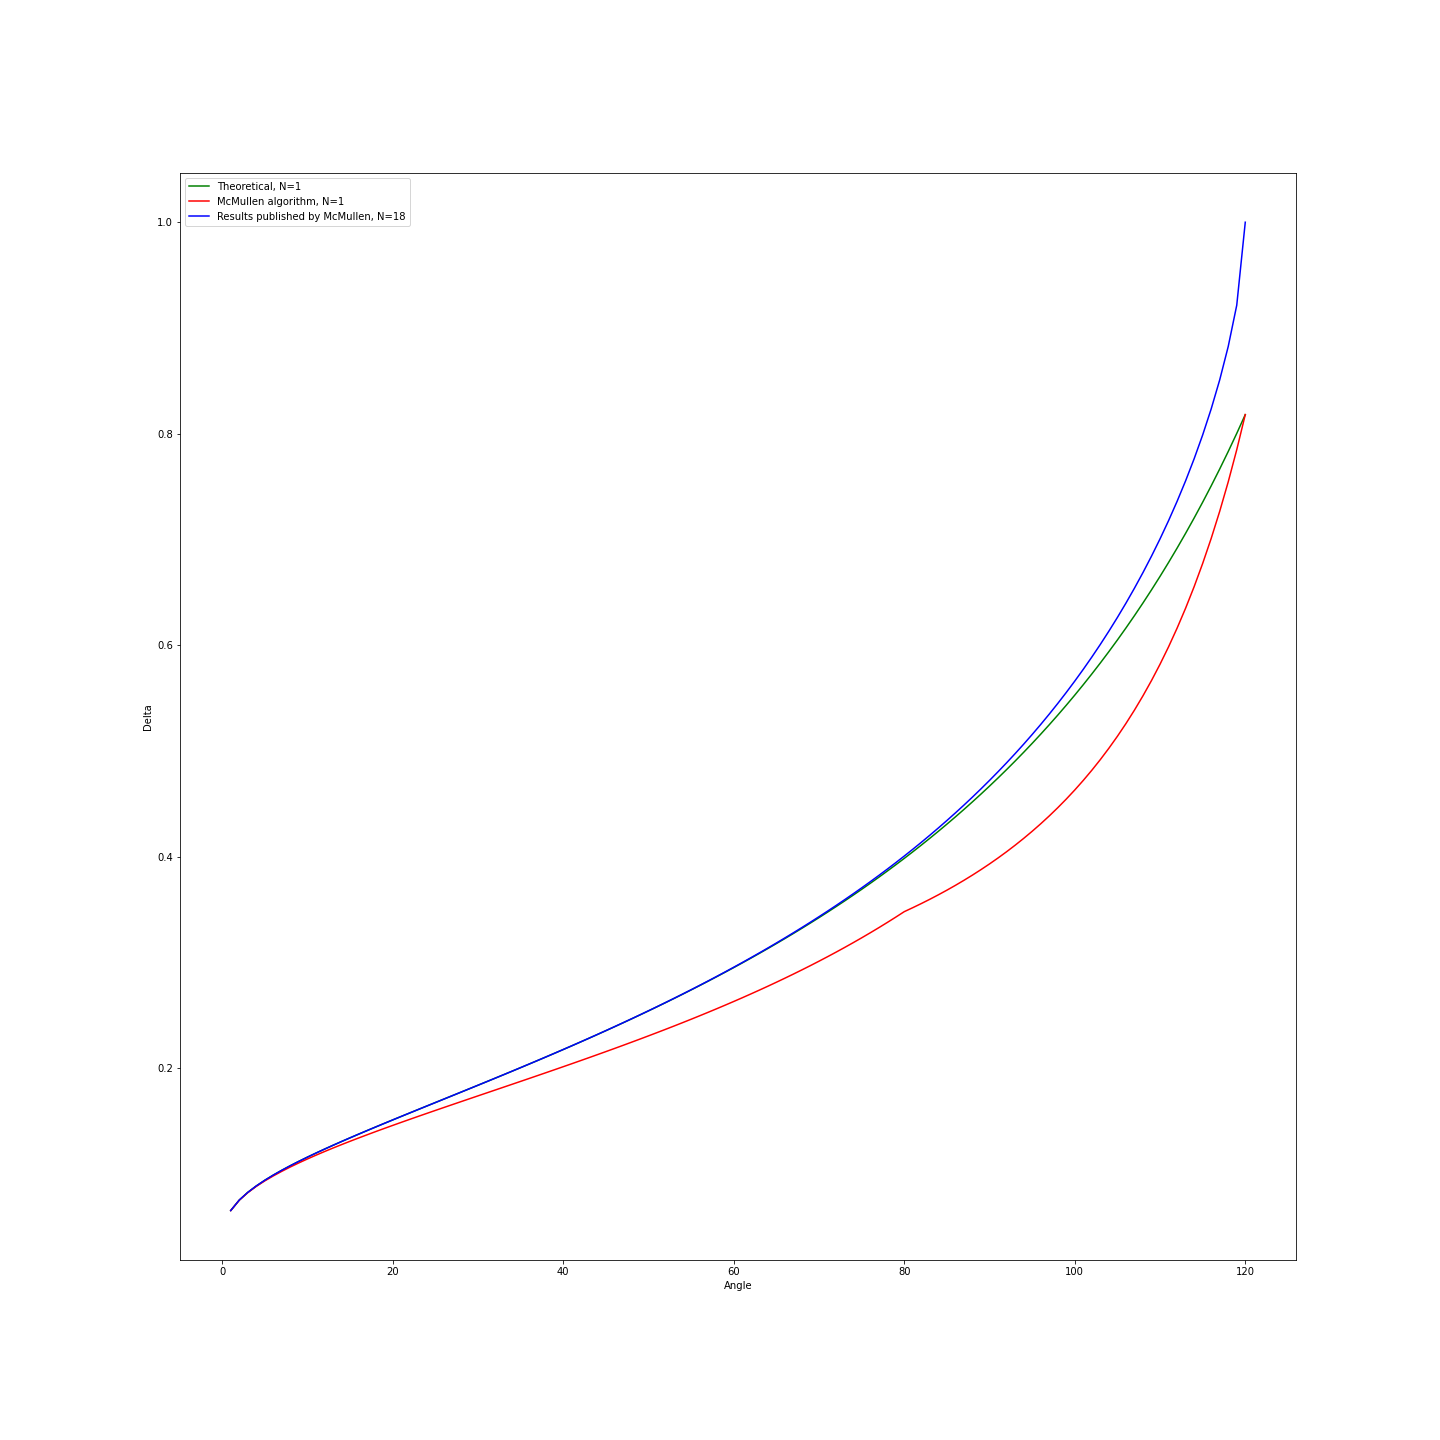
\includegraphics[width=0.8\textwidth]{McMullens example.png}
\caption{Level 1 ($N=1$) approximations, including McMullen's published data\cite{mcmullen1998hausdorff}[Table 12] (colored in blue), our $N=1$ theoretical approximation (green), and $N=1$ numerical approximation based on McMullen's algorithm (red). The angle $\theta$ is running from $1^\circ$ to $120^\circ$. }
\end{figure}

In the above figure, we plotted three results together, including the data published by McMullen \cite{mcmullen1998hausdorff}[Table 12] for $N=18$ which is colored in blue, the output of our implementation for $N=1$ which is colored in red, and the theoretical result $
\delta(G)\approx \alpha=\frac{\ln\left(\frac{1}{2}\right)}{\ln\left(t \right)}
=\frac{\ln\left(\frac{1}{3}\right)}{\ln\left(\frac{\tan^2\left(\frac{\theta}{2}\right)}{2+\left(\tan^2\left(\frac{\theta}{2}\right)\right)+\sec\left(\frac{\theta}{2}\right)} \right)}
$ for $N=1$ which is colored in green.


We can see that the $N=1$ theoretical result can rather well resemble McMullen's $N=18$ finding\cite{mcmullen1998hausdorff} for $\theta\in [0^\circ,80^\circ]$. Furthermore, we can see that, owing to McMullen's practical concern, the outcome of our implementation's $N=1$ instance did not correspond with the theoretical findings or the $N=18$ results provided by McMullen.


This, however, may be improved angle by angle. It takes longer when $N$ exceeds $8$ (after $N>8$, each level may take more than 2 hours before parallel computing), but it is achievable.

For instance, if we focus on $\theta=50^\circ$, then we can have the following improvement
\begin{center}
\begin{table}[h]
\begin{tabular}{ c c c }
\hline
 level & degree & $\alpha_N(\Gamma)$ \\ \hline

 1 & 50 & 0.23066000000008990 \\
 2 & 50 & 0.27209000000013134 \\
 3 & 50 & 0.25797000000011720 \\
 4 & 50 & 0.24197000000010122 \\
 5 & 50 & 0.25848000000011770 \\
 6 & 50 & 0.25839000000011764 \\
 7 & 50 & 0.25825000000011750 \\  
 8 & 50 & 0.25839000000011764 \\  
 9 & 50 & 0.25839000000011764 \\ \hline
 
\end{tabular}
\caption{An improvement for the case $\theta=50^\circ$ with precision$=0.00001$.}
    \label{tab:McMullen1}   
\end{table}
\end{center}

The meaning of the above table is twofold: First and foremost, it demonstrates that if we fix a precision to a specific digit, the sequence of $\alpha_N$ would ultimately converge (in $O(N)$ time complexity). Second, we can observe an improvement when we compare the first two digits after the decimal point for the $N=1$ result, which is $0.23$, to McMullen's $N=18$ result, which is $0.25$, i.e. when $N>4$ the sequence becomes stable. Furthermore, the figure after $25$ may vary as our precision improves.



Furthermore, in the following table, for large $\theta$, i.e. $\theta\to\frac{2\pi}{3}$, we can observe that the sequence tends to converge to $1$.


\begin{center}
\begin{table}[h]
\begin{tabular}{ c c c }
\hline
 level & degree & $\alpha_N(\Gamma)$ \\ \hline

 1 & 120 & 0.8180799999989117 \\
 2 & 120 & 0.8739599999986574 \\
 3 & 120 & 0.9045899999985180 \\
 4 & 120 & 0.9240099999984296 \\
 5 & 120 & 0.9372899999983691 \\
 6 & 120 & 0.9468699999983256 \\
 7 & 120 & 0.9540399999982929 \\  
 8 & 120 & 0.9595799999982677 \\  
 9 & 120 & 0.9639899999982476 \\ \hline
 
\end{tabular}
\caption{Improve $\alpha_N(\Gamma)$ such that it converges to $\delta(\Gamma)=1$ with precision$=0.00001$.}
    \label{tab:McMullen}   
\end{table}
\end{center}

Based on the above observation, we can also notice that compared to $N=1$, the more level we can reach, the larger value $\alpha_N(\Gamma)$ will be, and different angles need different $N$ to converge when the same precision was given. Furthermore, based on these above results, including our $N=1$ theoretical formula can fit McMullen's result well for $\theta\leq 80^\circ$, and when $\theta>80^\circ$, as shown in the above two examples, we can have a good approximation compare to McMullen's results by increasing the number of level, $N$. 

Finally, we also use the same understanding to implement McMullen's algorithm for $m=2$ well-distributed Schottky group and plot the following results with the results generated by our main theorem and conjecture all together.

For $m=2$, by using cosine law for $\frac{\pi}{2}$, and solving $\alpha$ for $3(t)^\alpha=1$, we have the first level approximation as follows
$$
\delta(G)\approx \alpha=\frac{\ln\left(\frac{1}{3}\right)}{\ln\left(t \right)}
=\frac{\ln\left(\frac{1}{3}\right)}{\ln\left(\frac{\tan^2\left(\frac{\theta}{2}\right)}{2+\left(\tan^2\left(\frac{\theta}{2}\right)\right)} \right)}.
$$


\begin{figure}[H]
\centering
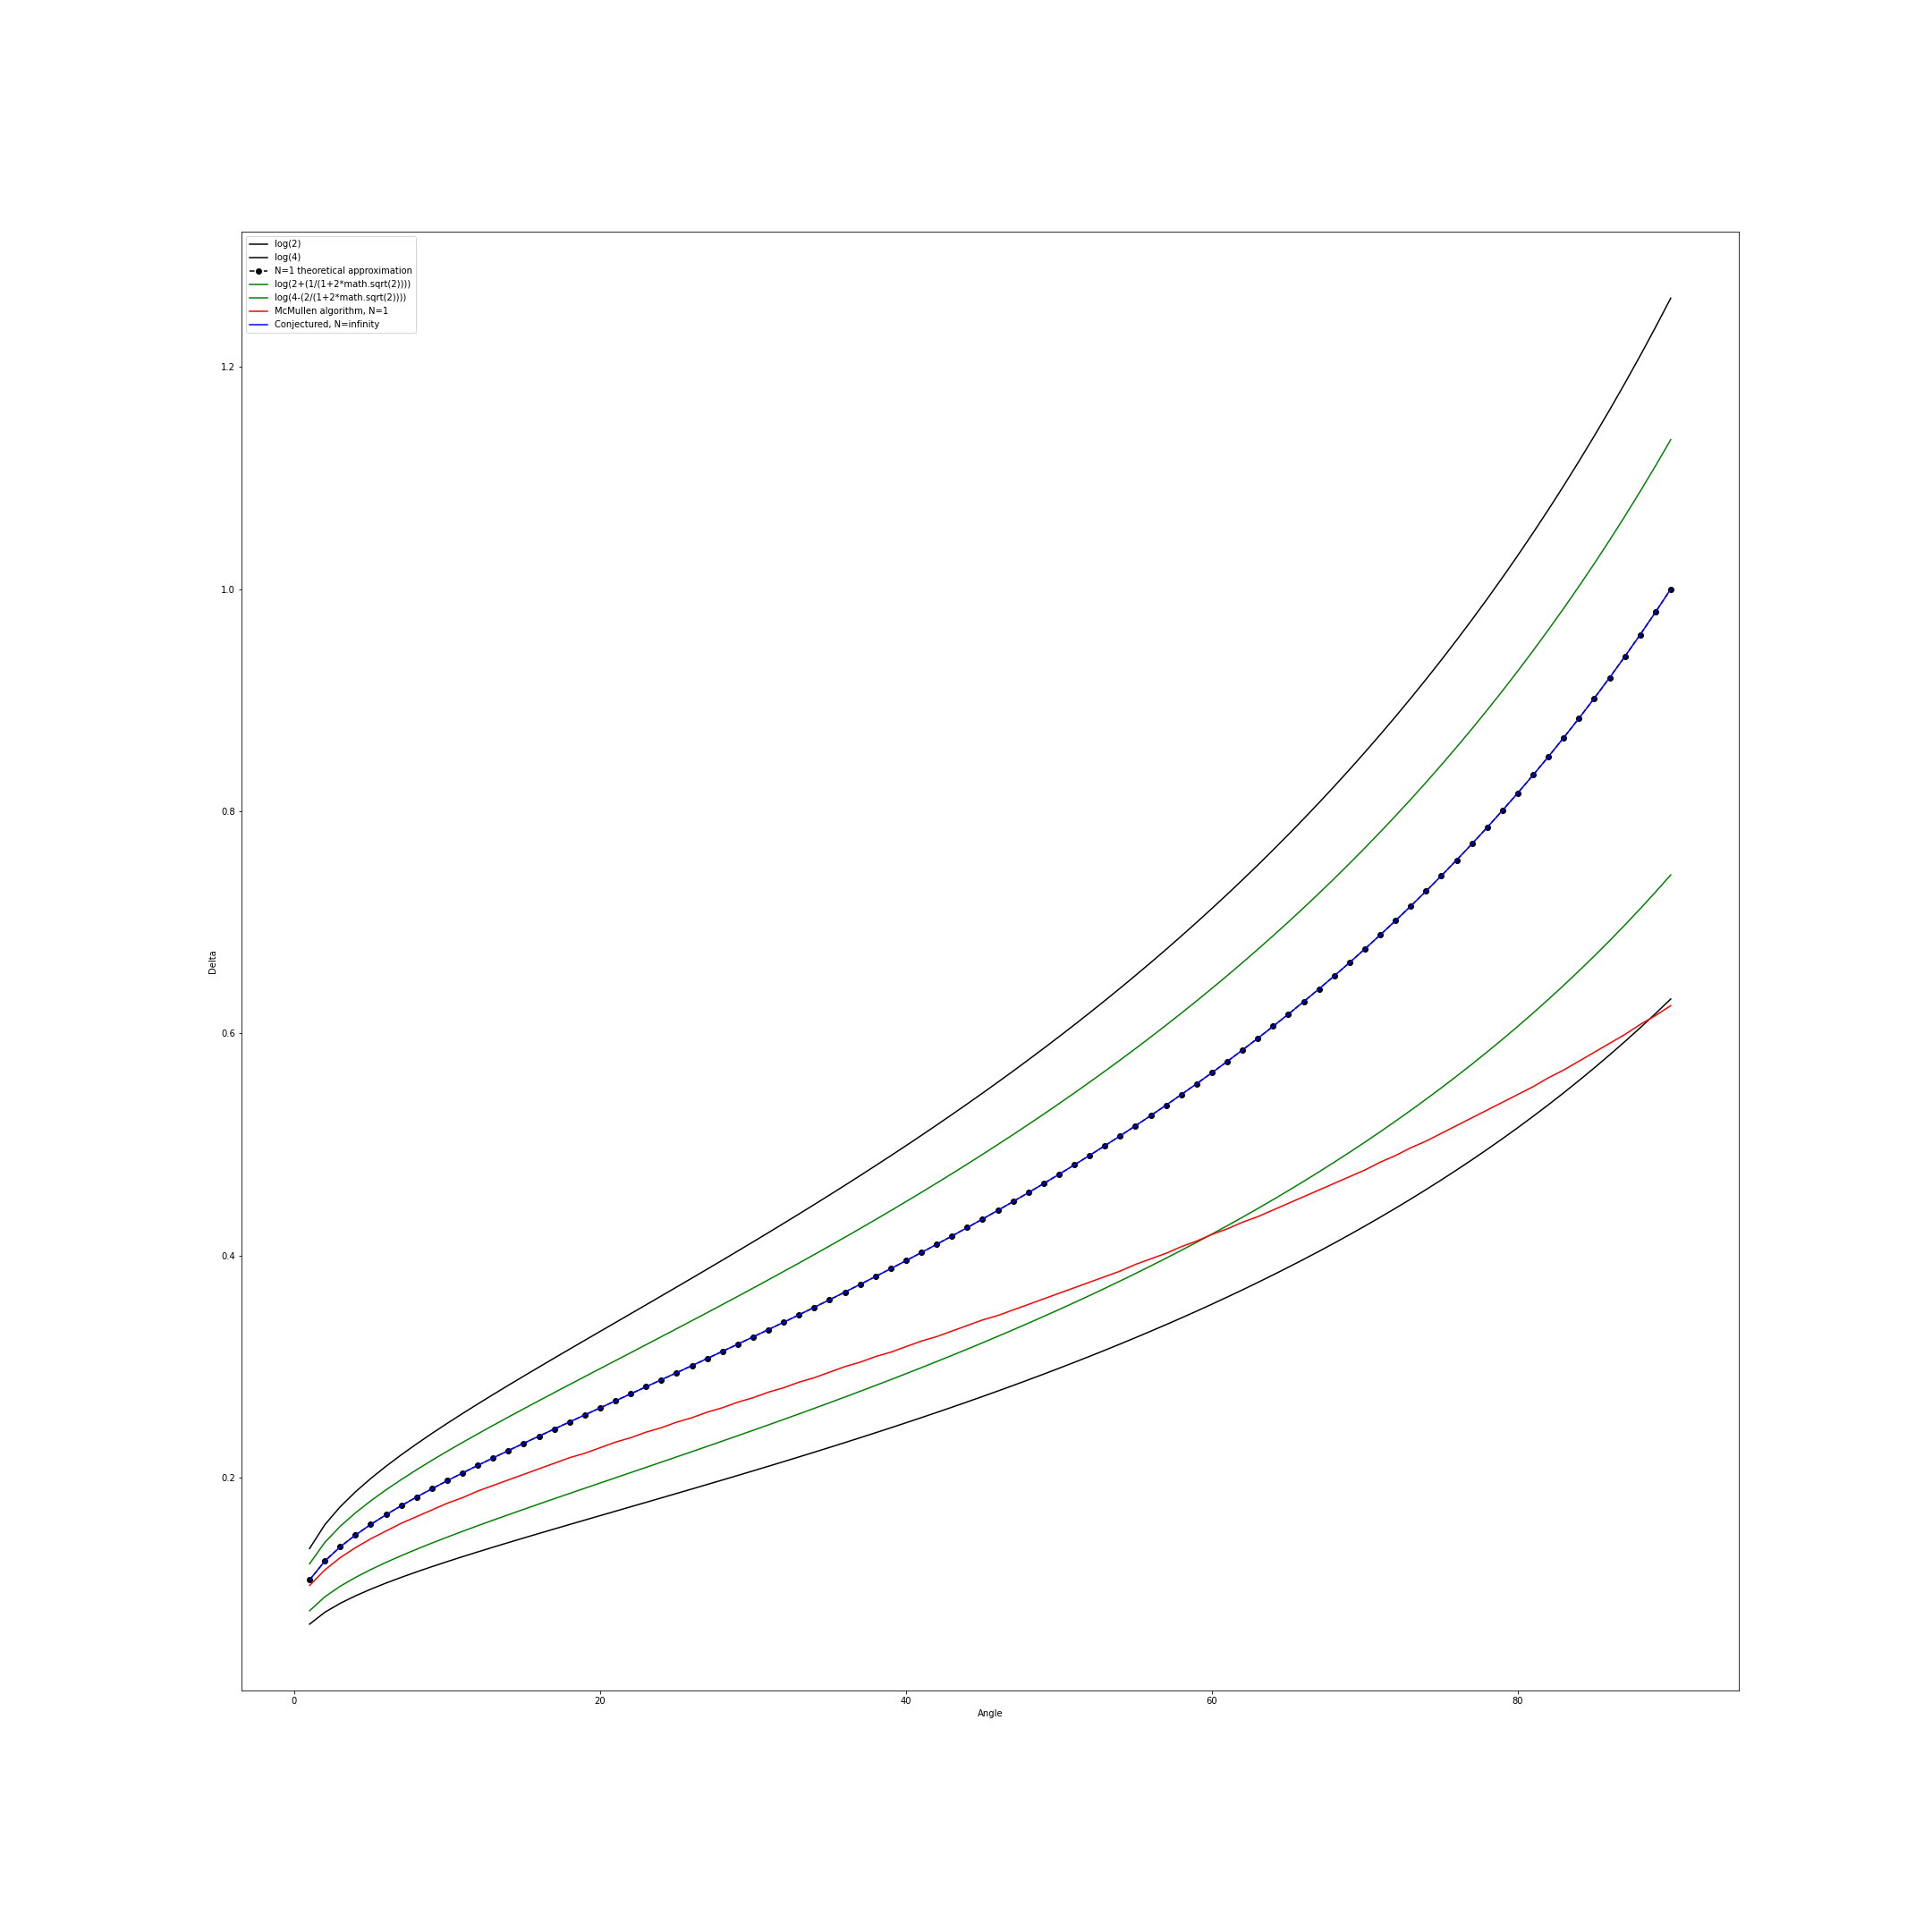
\includegraphics[width=1\textwidth]{Results from our main theorem, conjecture, and implementation of McMullen algorithm.png}
\caption{Results from our main theorems (colored in green and black), conjecture (blue), theoretical $N=1$ approximation (dotted black), and numerical $N=1$ approximation implementation of McMullen algorithm (red).}
\end{figure}

Although we have not had enough time to improve the results of our implementation of McMullen's algorithm, based on the above examples, we believe that once $N$ increases, the curve will be shifted towards the conjectured curve.

Surprisingly, the findings of the $N=1$ approximation precisely match our conjecture for $N\to \infty$. Therefore, if our conjecture is true, then this implies that for a well-distributed Schottky group of rank $2$, $\delta(\Gamma)=\alpha_1(\Gamma)$. It may also imply that for all $N$, we have $$\delta(\Gamma)=\alpha_N(\Gamma)=\alpha_1(\Gamma)=\frac{\ln\left(\frac{1}{3}\right)}{\ln\left(\frac{\tan^2\left(\frac{\theta}{2}\right)}{2+\left(\tan^2\left(\frac{\theta}{2}\right)\right)} \right)}=\frac{\ln\left(3\right)}{\ln\left(\cosh\left(r\right)\right)},$$ where
$$
r=\ln\left(\frac{1+\cos\left(\frac{\theta}{2}\right)}{1-\cos\left(\frac{\theta}{2}\right)} \right),
$$
since $T0=\cos\left(\frac{\theta}{2}\right).$
For the last equation, it can be demonstrated that
$$
\cosh(r)=\frac{1+\cos^2\left(\frac{\theta}{2}\right)}{\sin^2\left(\frac{\theta}{2}\right)},
$$
and
$$
\frac{\tan^2\left(\frac{\theta}{2}\right)}{2+\left(\tan^2\left(\frac{\theta}{2}\right)\right)} = \left(\frac{1+\cos^2\left(\frac{\theta}{2}\right)}{\sin^2\left(\frac{\theta}{2}\right)}\right)^{-1}.
$$
Hence, we always have $\frac{\ln\left(\frac{1}{3}\right)}{\ln\left(\frac{\tan^2\left(\frac{\theta}{2}\right)}{2+\left(\tan^2\left(\frac{\theta}{2}\right)\right)} \right)}=\frac{\ln\left(3\right)}{\ln\left(\cosh\left(r\right)\right)}$ for all $0<\theta<\frac{\pi}{2}$.
This alternate strategy might also shed some light on the meaning of $cosh(r)$ in our conjecture. A proof of the conjecture, a generalization to $m>2$, and enhancements to our implementations are on the horizon for our future work. Due to heavy matrix operations involved, an implementation on parallel computing in a contemporary computer might potentially enhance McMullen's results.


Our source code can be downloaded from GitHub: \newline
{\footnotesize \url{https://github.com/williamchuang/well-distributed-schottky-groups/tree/main/code}}

% Bibliography (calls up the entries in thesis.bib if you run bibTeX):
\bibliographystyle{amsplain}
\addcontentsline{toc}{chapter}{Bibliography}
\singlespacing
\bibliography{thesis}
%\bibliography{qhe.bib}
\end{document}


